\documentclass{elsarticle}

\usepackage{amsmath}
\usepackage{hyperref}
\usepackage{subcaption}
\usepackage{tikz}     % for tikz pictures
\usetikzlibrary{calc} % for computing points in tikz pictures
\usetikzlibrary{shapes.geometric}

% equation punctuation
\newcommand{\eqp}{\,.} % equation period
\newcommand{\eqc}{\,,} % equation comma

% derivatives
\newcommand{\dd}[2]{\frac{d #1}{d #2}}               % ordinary derivative
\newcommand{\pd}[2]{\frac{\partial #1}{\partial #2}} % partial derivative
\newcommand{\ppt}[1]{\pd{#1}{t}}                     % partial d/dt
\newcommand{\ppx}[1]{\pd{#1}{x}}                     % partial d/dx
\newcommand{\ppy}[1]{\pd{#1}{y}}                     % partial d/dy
\newcommand{\ddt}[1]{\frac{d#1}{dt}}                 % ordinary d/dt

% phase-space arguments
\newcommand{\x}{\mathbf{x}}
\newcommand{\di}{\mathbf{\Omega}}
\newcommand{\xt}{(\x,t)}
\newcommand{\xet}{(\x,E,t)}
\newcommand{\xdet}{(\x,\di,E,t)}

% transport quantities
\newcommand{\aflux}{\psi}
\newcommand{\totalxsec}{\Sigma_\textup{t}}
\newcommand{\scatteringxsec}{\Sigma_\textup{s}}
\newcommand{\fissionxsec}{\Sigma_\textup{f}}
\newcommand{\Qext}{Q_\textup{ext}}
\newcommand{\Qtot}{Q_\textup{tot}}

% domain
\newcommand{\domain}{\mathcal{D}}
\newcommand{\normalvector}{\mathbf{n}}
\newcommand{\incoming}{u^{\textup{inc}}}

% linear system
\newcommand{\U}{\mathbf{U}}
\newcommand{\A}{\mathbf{A}}
\newcommand{\D}{\mathbf{D}}
\newcommand{\ssrhs}{\mathbf{b}}
\newcommand{\M}{\mathbf{M}}
\newcommand{\dt}{\Delta t}

% FCT
\newcommand{\p}{\mathbf{p}}
\renewcommand{\P}{\mathbf{P}}

% integrals and sums
\newcommand{\sumj}{\sum\limits_j}
\newcommand{\sumjnoti}{\sum\limits_{j\ne i}}
\newcommand{\sumKSij}[1][K]{\sum\limits_{#1\in\mathcal{K}(S_{i,j})}}
\newcommand{\intSi}{\int\limits_{S_i}}
\newcommand{\intSij}{\int\limits_{S_{i,j}}}

% FEM
\newcommand{\test}{\varphi}

% indices
\newcommand{\indices}{\mathcal{I}}

% theorem environments
\newtheorem{thm}{Theorem}
\newtheorem{lem}[thm]{Lemma}
\newdefinition{defn}{Definition}
\newdefinition{rmk}{Remark}
\newproof{prf}{Proof}

% parentheses
\newcommand{\pr}[1]{\left(#1\right)}

\newcommand{\tcr}[1]{\textcolor{red}{#1}}

\begin{document}
%------------------------------------------------------------------------------
\begin{frontmatter}

\journal{Journal of Computational and Applied Mathematics}

\title{Application of the Entropy Viscosity Method and the Flux-Corrected Transport
  Algorithm to the Transport Equation using Continuous Finite Elements}

\author[tamu]{Joshua E. Hansel}
\ead{joshhansel@tamu.edu}

\author[tamu]{Jean C. Ragusa}
\ead{jean.ragusa@tamu.edu}

\address[tamu]{Texas A\&M University,
  400 Bizzell St,
  College Station, TX 77840}

\begin{abstract}
The Flux-Corrected Transport (FCT) algorithm is
applied to the unsteady and steady-state particle transport equation. The proposed FCT method employs the following:
(1) a low-order, positivity-preserving scheme,
based on the application of M-matrix properties,
(2) a high-order scheme based on the entropy viscosity method introduced by
Guermond \cite{guermond_ev}, and
(3) local, discrete solution bounds derived from the integral transport equation.
The resulting scheme is second-order accurate in space,
enforces an entropy inequality, mitigates the formation of spurious
oscillations, and guarantees the absence of negativities.
Space discretization is achieved using  continuous finite elements. 
Time discretizations for unsteady problems include theta schemes
such as explicit and implicit Euler, and strong-stability preserving
Runge-Kutta (SSPRK) methods.
The developed scheme is shown to be robust with explicit time discretizations
but encounters nonlinear convergence difficulties for steady-state
and implicit time discretizations.
\end{abstract}


\begin{keyword}
entropy viscosity \sep FCT \sep CGFEM \sep transport equation
\end{keyword}

\end{frontmatter}
%------------------------------------------------------------------------------
\tcr{should we ask Guermond to be a 3rd author?}

\section{Introduction\label{sec:introduction}}
The transport equation, also called the Boltzmann equation, describes the
transport of particles or waves through some background media and some
of its applications include nuclear reactors, atmospheric science, radiation
therapy, astrophysics, radiation shielding, and high energy density physics.
In this paper, focus is on solution techniques applicable to the first-order
form of the transport equation, discretized in angle with discrete ordinates,
which gives what is commonly called the $S_N$ equations:
\begin{equation}\label{eq:transport_scalar}
  \frac{1}{v(E)}\ppt{\aflux} + \di\cdot\nabla\aflux\xdet
    + \totalxsec\xet\aflux\xdet = \Qtot\xdet
  \eqc
\end{equation}
where $\Qtot\xdet$ denotes the sum of the extraneous source, prompt and delayed
fission sources, and scattering source:
\begin{multline}
  \Qtot\xdet \equiv \Qext\xdet\\
    + \frac{\chi_\text{p}(E)}{4\pi}\int\limits_0^\infty
      dE'\nu_\text{p}(\x,E',t)\fissionxsec(\x,E',t)\phi(\x,\di,E',t)
    + \sum\limits_{i=1}^{n_\text{d}}\frac{\chi_{\text{d},i}(E)}{4\pi}\lambda_i C_i\xt\\
    + \int\limits_0^\infty dE'\int\limits_{4\pi}d\di'
      \scatteringxsec(\x,E'\rightarrow E,\di'\rightarrow\di,t)\aflux(\x,\di',E',t)
  \eqp
\end{multline}
The $S_N$ equations are an attractive form of the transport equation because
the $S_N$ equations can be decoupled by using iterative techniques for the
scattering source, an approach called source iteration \cite{glasstone}:
\begin{equation}
  \frac{1}{v}\ppt{\aflux^{(\ell)}}
    + \di\cdot\nabla\aflux^{(\ell)}
    + \totalxsec\aflux^{(\ell)} = \Qtot^{(\ell-1)} \eqc
\end{equation}
where $\ell$ is the iteration index. The decoupling of the equations allows
scalar solution techniques to be leveraged.
Traditionally, the preferred spatial discretization method for the $S_N$
equations is the Discontinuous Galerkin finite element method (DGFEM)
\cite{Lesaint1974}\cite{Reed_Hill_1973}. Here, however, the
Continuous Galerkin finite element method (CGFEM) is applied. There
has been some recent work by Guermond and Popov \cite{guermond_ev} on
solution techniques for conservation laws with CGFEM, which addresses some
of the main disadvantages of CGFEM versus DGFEM, including the formation
of spurious oscillations. This work aims to demonstrate a proof of concept
for the application of these solution techniques to the transport equation.
Furthermore, some or all of the methodology explored in this paper may be
later extended to DGFEM as well \cite{zingan_2013}.

One of the main objectives of this paper is to present a method that precludes
the formation of spurious oscillations and the negativities that result from
these oscillations. The occurrence of negativities in the numerical solution of
the transport equation has been a long-standing issue \cite{lanthrop}.
Not only are these negativities physically inaccurate, but they can cause
simulations to terminate prematurely. Many attempts to remedy this
issue rely on ad-hoc fix-ups, such as the set-to-zero fix-up for the
classic diamond difference scheme \cite{lewis}. Recent work by Hamilton
introduced a similar fix-up for the linear discontinuous finite element
method (LDFEM) that conserves local balance and preserves third-order accuracy.
Walters and Wareing developed characteristic methods \cite{walters_NC}, but
Wareing later notes that these characteristic methods are difficult to
implement and offers a nonlinear positive spatial differencing scheme
known as the exponential discontinuous scheme \cite{wareing}.
Maginot has recently developed a consistent set-to-zero (CSZ) LDFEM
method \cite{maginot}, as well as a non-negative method for bilinear
discontinuous FEM \cite{maginot_mc2015}.

Traditional approaches to remedy the spurious oscillation issue included
the flux-corrected transport (FCT) algorithm, introduced in 1973 for finite
difference discretizations
by Boris and Book \cite{borisbook}, which has since been applied to the finite
element method \cite{kuzmin_FCT}. The idea of FCT is to blend a low-order scheme
having desirable properties with a scheme of a higher order of accuracy.

Recent work by Guermond and Popov addresses the issue of spurious oscillations
for general conservation laws by using artificial dissipation based on
local entropy production, a method known as entropy viscosity \cite{guermond_ev}.
The idea of entropy viscosity is to enforce an entropy inequality on the weak solution,
and thus filter out weak solutions containing spurious oscillations. However,
entropy viscosity solutions may still contain spurious
oscillations, albeit smaller in magnitude, and consequently negativities
are not precluded. To circumvent this deficiency, Guermond proposed using
the entropy viscosity method in conjunction with the FCT
algorithm \cite{guermond_secondorder}; the high-order scheme component in FCT,
traditionally the unmodified Galerkin scheme, is replaced with the entropy
viscosity scheme.
For the low-order
scheme, Guermond also introduced
a discrete maximum principle (DMP) preserving (and positivity-preserving)
scheme for scalar
conservation laws \cite{guermond_firstorder}.

This paper presents an FCT scheme that is largely rooted in the work by Guermond
and Popov, but is extended to allow application to the transport equation,
which does not fit the prototype of a conservation law but is instead a
balance law, which includes sinks and sources, namely the reaction term
$\totalxsec\aflux$ and the source term $\Qtot$. The presence
of these terms is also a novelty in the context of the FCT algorithm.
In addition, much of the present work on FCT has been for fully explicit time
discretizations, although there has been some work on implicit time discretizations
as well. Because speeds in radiation transport (such as the speed of light)
are so large, implicit and steady-state time discretization are important
considerations, given the CFL time step size restriction for fully explicit
methods. Thus this paper also considers implicit and steady-state FCT, which
has been implemented before \cite{implicit_FCT}.

This paper is organized as follows. Section \ref{sec:preliminaries} gives
some preliminaries such as the problem formulation and discretization.
Recall that the FCT algorithm uses a low-order scheme and a high-order scheme.
Section \ref{sec:low} presents the low-order scheme, Section \ref{sec:high}
presents the high-order scheme (which is based on entropy viscosity),
and Section \ref{sec:fct} presents the FCT scheme that combines the two. Then, Section
\ref{sec:results} presents results for a number of test problems, and
Section \ref{sec:conclusions} gives conclusions.


\section{Preliminaries\label{sec:preliminaries}}
For the remainder of this paper, the scalar transport model given by
Equation \eqref{eq:transport_scalar} will be generalized to a scalar
balance equation having reaction terms and source terms, with the following
notation:
\begin{equation}\label{eq:scalar_model}
  \ppt{u} + v\di\cdot\nabla u\xt
    + \sigma(\x) u\xt = q\xt
  \eqc
\end{equation}
where $u$ is the balanced quantity, $v$ is the transport speed, $\di$ is
a constant, uniform unit direction vector, $\sigma$ is the reaction coefficient,
and $q$ is the source function.

The problem formulation is completed by supplying initial conditions
(for transient problems):
\begin{equation}
  u(\x,0) = u^0(\x) \quad \x\in\domain \eqc
\end{equation}
where $\domain$ denotes the problem domain, as well as boundary conditions,
which will be assumed to be incoming flux boundary conditions:
\begin{equation}
  u\xt = \incoming\xt \quad \x\in\partial\domain^- \eqc
\end{equation}
where $\incoming\xt$ is the incoming boundary data function, and
$\partial\domain^-$ is the incoming portion of the domain boundary:
\begin{equation}
  \partial\domain^- \equiv \{ \x\in\partial\domain :
  \normalvector(\x)\cdot\di \leq 0 \} \eqc
\end{equation}
where $\normalvector(\x)$ is the outward-pointing normal vector on the domain
boundary at point $\x$.

Application of the standard Galerkin method with linear basis functions
gives the following semi-discrete system:
\begin{subequations}
  \begin{equation}
    \M^C\ddt{\U} + \A\U(t) = \ssrhs(t) \eqc
  \end{equation}
  \begin{equation}
    M^C_{i,j} \equiv \intSij \test_i(\x)\test_j(\x) dV \eqc
  \end{equation}
  \begin{equation}
    A_{i,j} \equiv \intSij\left(
    v\di\cdot\nabla\test_j(\x) +
    \sigma(\x)\test_j(\x)\right)\test_i(\x) dV \eqc
  \end{equation}
  \begin{equation}
    b_i(t) \equiv \intSi q(\x)\test_i(\x) dV \eqc
  \end{equation}
\end{subequations}
where $U_j(t)$ are the degrees of freedom of the approximate solution $u_h$:
\begin{equation}
  u_h\xt = \sumj U_j(t) \test_j(\x) \eqp
\end{equation}

A number of temporal discretizations are considered in this paper.
Fully explicit temporal discretizations considered include forward Euler:
\begin{equation}
  \M^C\frac{\U^{n+1}-U^n}{\dt} + \A\U^n = \ssrhs^n \eqc
\end{equation}
as well as Strong Stability Preserving Runge Kutta (SSPRK) methods that
can be expressed in the following form:
\begin{subequations}\label{eq:ssprk}
\begin{align}
  & \hat{\U}^0 = \U^n \eqc \\
  & \hat{\U}^i = \gamma_i \U^n + \zeta_i \left[
      \hat{\U}^{i-1}
      + \dt\mathbf{G}(t^n+c_i\dt, \hat{\U}^{i-1})\right]
    \eqc \quad
    i = 1,\ldots,s
    \eqc \\
  & \U^{n+1} = \hat{\U}^s \eqp
\end{align}
\end{subequations}
where $s$ is the number of stages, $\gamma_i$, $\zeta_i$, and $c_i$ are
coefficients that correspond to the particular SSPRK method, and
$\mathbf{G}$ represents the right-hand-side function of an ODE
\begin{equation}
  \ddt{\U} = \mathbf{G}(t,\U(t)) \eqc
\end{equation}
which in this case is the following:
\begin{equation}
  \mathbf{G}(t,\U(t)) = (\M^C)^{-1}
    \left(\ssrhs(t) - \A\U(t)\right) \eqp
\end{equation}
The form given in Equation \eqref{eq:ssprk} makes it clear that these
SSPRK methods can be expressed as a linear combination of steps resembling
forward Euler steps, with the only difference being that the explicit
time dependence of the source is not necessarily the old time $t^n$ but
instead is a stage time $t^n + c_i\dt$. The 3-stage, 3rd-order accurate SSPRK
method has the following coefficients:
\begin{equation}
  \gamma = \left[\begin{array}{c}
    0\\\frac{3}{4}\\\frac{1}{3}\end{array}\right]
  \eqc \quad
  \zeta = \left[\begin{array}{c}
    1\\\frac{1}{4}\\\frac{2}{3}\end{array}\right]
  \eqc \quad
  c = \left[\begin{array}{c}0\\1\\\frac{1}{2}\end{array}\right] \eqp
\end{equation}
SSPRK methods are a subclass of Runge Kutta methods that offer high-order
accuracy while preserving stability \cite{gottlieb}\cite{macdonald}.
The theta method is also considered for temporal discretization:
\begin{equation}
  \M^C\frac{\U^{n+1}-U^n}{\dt} + \A((1-\theta)\U^n + \theta\U^{n+1})
  = (1-\theta)\ssrhs^n + \theta\ssrhs^{n+1} \eqc
\end{equation}
where $0\leq\theta\leq 1$ is the implicitness parameter, where for example
$\theta$ values of $0$, $\frac{1}{2}$, and $1$ correspond to forward Euler,
Crank-Nicolson, and backward Euler, respectively. Finally, the steady-state
case is also considered:
\begin{equation}
  \A\U = \ssrhs \eqp
\end{equation}


\section{FCT Methodology Applied to Particle Transport\label{sec:methodology}}
\documentclass{mathnotes}
\usepackage{color}
\usepackage{xcolor}
\usepackage{alltt}
\usepackage{amsmath}
\usepackage{amssymb}
\title{Maximum-Principle Preserving Finite Element Method for the
  Radiation Transport Equation}
\author{Jean-Luc Guermond\\Jean Ragusa\\Joshua Hansel}

% required packages
\usepackage{xcolor}

% general
\newcommand{\x}{\mathbf{x}}
\newcommand{\timevalue}{t}
\newcommand{\timestepsize}{\Delta\timevalue}
\newcommand{\timeindex}{n}
\newcommand{\speed}{v}
\newcommand{\velocity}{\mathbf{\speed}}
\newcommand{\normalvector}{\mathbf{n}}

% solution
\newcommand{\scalarsolution}{u}
\newcommand{\vectorsolution}{\mathbf{\scalarsolution}}
\newcommand{\approximatescalarsolution}{\tilde{\scalarsolution}}
\newcommand{\solutionletter}{U}
\newcommand{\solutionvector}{\mathbf{\solutionletter}}
\newcommand{\lowordersolution}[1][]{
  \ifthenelse{\equal{#1}{}}{\solutionvector^L}{\solutionvector^{L,#1}}}
\newcommand{\highordersolution}[1][]{
  \ifthenelse{\equal{#1}{}}{\solutionvector^H}{\solutionvector^{H,#1}}}

% domain and FEM
\newcommand{\domain}{\mathcal{D}}
\newcommand{\domainboundary}{\partial\domain}
\newcommand{\cellindex}{K}
\newcommand{\cell}{K}
\newcommand{\volume}{V}
\newcommand{\testfunction}{\varphi}
\newcommand{\support}{S}
\newcommand{\maxdof}{N}

% local viscous bilinear form
\newcommand{\localviscbilinearform}[3]{b_#1(\testfunction_#2, \testfunction_#3)}
\newcommand{\cellvolume}{\volume_\cellindex}
\newcommand{\cardinality}[1][]{\ifthenelse{\equal{#1}{}}{n_\cell}{n_#1}}
\newcommand{\indicescell}[1][]{\ifthenelse{\equal{#1}{}}{\mathcal{I}(\cell)}
  {\mathcal{I}(#1)}}

% entropy viscosity
\newcommand{\entropy}{\eta}
\newcommand{\entropyjump}{\mathcal{J}}
\newcommand{\entropyresidual}{\mathcal{R}}
\newcommand{\entropyresidualcoef}{c_\entropyresidual}
\newcommand{\entropyjumpcoef}{c_\entropyjump}

% conservation law
\newcommand{\consfluxletter}{f}
\newcommand{\consfluxscalar}[1][\scalarsolution]{\mathbf{\consfluxletter}(#1)}
\newcommand{\consfluxvector}{\mathbf{\MakeUppercase{\consfluxletter}}
  (\vectorsolution)}
\newcommand{\conssource}{\mathbf{s}(\vectorsolution)}

% viscosity
\newcommand{\viscosity}{\nu}
\newcommand{\cellviscosity}{\viscosity_\cellindex}
\newcommand{\lowordercellviscosity}[1][]{
  \ifthenelse{\equal{#1}{}}{\cellviscosity^L}
  {\cellviscosity^{L,#1}}}
\newcommand{\highordercellviscosity}[1][]{
  \ifthenelse{\equal{#1}{}}{\cellviscosity^H}
  {\cellviscosity^{H,#1}}}
\newcommand{\entropycellviscosity}[1][]{
  \ifthenelse{\equal{#1}{}}{\cellviscosity^\entropy}
  {\cellviscosity^{\entropy,#1}}}

% viscous fluxes
\newcommand{\viscstring}{\text{visc}}
\newcommand{\viscflux}[1]{\mathbf{\consfluxletter}^{\viscstring,#1}}
\newcommand{\viscconsfluxvector}
  {\mathbf{\MakeUppercase{\consfluxletter}}^\viscstring
  (\vectorsolution,\viscosity)}

% mass matrix
\newcommand{\massmatrixletter}{M}
\newcommand{\massmatrix}{\mathbf{\massmatrixletter}}
\newcommand{\consistentmassmatrix}{\massmatrix^C}
\newcommand{\lumpedmassmatrix}{\massmatrix^L}
\newcommand{\lumpedmassentry}{\massmatrixletter^L_{i,i}}

% steady-state system matrix and rhs
\newcommand{\ssmatrixletter}{A}
\newcommand{\ssmatrix}[1][]{
  \ifthenelse{\equal{#1}{}}
  {\mathbf{\ssmatrixletter}}
  {\mathbf{\ssmatrixletter}^#1}}
\newcommand{\loworderssmatrix}[1][]{
  \ifthenelse{\equal{#1}{}}
  {\ssmatrix^L}
  {\ssmatrix^{L,#1}}}
\newcommand{\highorderssmatrix}[1][]{
  \ifthenelse{\equal{#1}{}}
  {\ssmatrix^H}
  {\ssmatrix^{H,#1}}}
\newcommand{\ssrhsletter}{b}
\newcommand{\ssrhs}[1][]{
  \ifthenelse{\equal{#1}{}}
  {\mathbf{\ssrhsletter}}
  {\mathbf{\ssrhsletter}^#1}}
\newcommand{\ssresletter}{r}
\newcommand{\ssres}{\mathbf{\ssresletter}}

% diffusion matrix
\newcommand{\diffusionmatrixletter}{D}
\newcommand{\diffusionmatrix}[1][]{
  \ifthenelse{\equal{#1}{}}
  {\mathbf{\diffusionmatrixletter}}
  {\mathbf{\diffusionmatrixletter}^#1}}
\newcommand{\loworderdiffusionmatrix}[1][]{
  \ifthenelse{\equal{#1}{}}
  {\diffusionmatrix^L}
  {\diffusionmatrix^{L,#1}}}
\newcommand{\highorderdiffusionmatrix}[1][]{
  \ifthenelse{\equal{#1}{}}
  {\diffusionmatrix^H}
  {\diffusionmatrix^{H,#1}}}

% Runge-Kutta
\newcommand{\RKstagesolution}{\hat{\mathbf{\solutionletter}}}
\newcommand{\RKintermediatesolution}{\tilde{\mathbf{\solutionletter}}}
\newcommand{\RKoldsolutioncoef}{\alpha}
\newcommand{\RKstagesolutioncoef}{\beta}
\newcommand{\RKtimecoef}{c}
\newcommand{\RKstagetime}{\hat{\timevalue}}
\newcommand{\RKnstages}{s}

% FCT
\newcommand{\DMPbound}{W}
\newcommand{\DMPboundsi}{\DMPbound^\pm_i}
\newcommand{\limitedfluxbound}{Q}
\newcommand{\limitedfluxboundsi}{\limitedfluxbound^\pm_i}
\newcommand{\limiterletter}{L}
\newcommand{\limitermatrix}{\mathbf{\limiterletter}}
\newcommand{\correctionfluxletter}{p}
\newcommand{\correctionfluxvector}{\mathbf{\correctionfluxletter}}
\newcommand{\correctionfluxij}{\MakeUppercase{\correctionfluxletter}_{i,j}}
\newcommand{\correctionfluxmatrix}{\mathbf{\MakeUppercase{\correctionfluxletter}}}
\newcommand{\correctionfluxsumsi}{\MakeUppercase{\correctionfluxletter}^\pm_i}
\newcommand{\limitedfluxsum}{\limitermatrix\cdot\correctionfluxmatrix}
\newcommand{\limitedfluxsumi}{\sumj\limiterletter\ij
  \MakeUppercase{\correctionfluxletter}\ij}

% radiation transport
\newcommand{\angularflux}{\psi}
\newcommand{\speedoflight}{c}
\newcommand{\totalcrosssection}{\Sigma_t}
\newcommand{\reactioncoef}{\sigma}
\newcommand{\directionvector}{\mathbf{\Omega}}
\newcommand{\scalarsource}{q}
\newcommand{\radiationsource}{Q}

% Euler equations
\newcommand{\density}{\rho}
\newcommand{\totalenergy}{E}
\newcommand{\momentum}{\mathbf{m}}
\newcommand{\pressure}{p}
\newcommand{\gasconstant}{\gamma}
\newcommand{\identity}{\mathbf{I}}

% shallow water equations
\newcommand{\height}{h}
\newcommand{\heightmomentum}{\mathbf{q}}
\newcommand{\bathymetry}{b}
\newcommand{\gravity}{g}
\newcommand{\speedofsound}{a}

%==============================================================================
% colors
\colorlet{lightBlue}{blue!10!white}
\colorlet{lightGreen}{green!10!white}

% sums and integrals
\renewcommand{\ij}{_{i,j}}
\newcommand{\sumj}{\sum\limits_j}
\newcommand{\sumjnoti}{\sum\limits_{j\ne i}}
\newcommand{\sumKSi}{\sum\limits_{\cellindex\subset\support_i}}
\newcommand{\sumKSij}{\sum\limits_{\cellindex\subset\support_{i,j}}}
\newcommand{\intSi}{\int\limits_{\support_i}}
\newcommand{\intSij}{\int\limits_{\support_{i,j}}}

% common fractions
\newcommand{\half}{\frac{1}{2}}

% derivatives
\newcommand{\dd}[2]{\frac{d #1}{d #2}}               % ordinary derivative
\newcommand{\pd}[2]{\frac{\partial #1}{\partial #2}} % partial derivative
\newcommand{\ppt}[1]{\pd{#1}{t}}                     % partial d/dt
\newcommand{\ddt}[1]{\frac{d#1}{dt}}                 % ordinary d/dt

% typesetting
\newcommand{\pr}[1]{\left(#1\right)} % parentheses
\newcommand{\sq}[1]{\left[#1\right]} % square brackets
\newcommand{\tab}{\hspace*{0.5cm}}   % tab for verbatim evironments
\newcommand{\eqp}{\,.} % equation period
\newcommand{\eqc}{\,,} % equation comma

% miscellaneous
\newcommand{\xt}{\pr{\x,\timevalue}}
\newcommand{\divergence}{\nabla\cdot}

% command to highlight term in equation
\newcommand{\highlightblue}[1]{
  \colorbox{lightBlue}{$\displaystyle#1$}}
\newcommand{\highlightgreen}[1]{
  \colorbox{lightGreen}{$\displaystyle#1$}}

% QED symbol command
\newcommand{\qed}{\nobreak \ifvmode \relax \else
      \ifdim\lastskip<1.5em \hskip-\lastskip
      \hskip1.5em plus0em minus0.5em \fi \nobreak
      \vrule height0.75em width0.5em depth0.25em\fi}

% math environments
\newenvironment{proof}[1][Proof]{\begin{trivlist}
\item[\hskip \labelsep {\bfseries #1}]}{\end{trivlist}}
\newenvironment{example}[1][Example]{\begin{trivlist}
\item[\hskip \labelsep {\bfseries #1}]}{\end{trivlist}}
\newenvironment{remark}[1][Remark]{\begin{trivlist}
\item[\hskip \labelsep {\bfseries #1}]}{\end{trivlist}}

% table environment
% #1 = caption
% #2 = label
% #3 = table format (columns)
% #4 = header row
\newenvironment{mytable}[4]
  {\begin{table}[htb]\caption{#1\label{tab:#2}}\begin{center}
    \begin{tabular}
    {#3}\hline #4\\\hline}
  {\hline\end{tabular}\end{center}\end{table}}

%==============================================================================
% Theorem environments for dissertation
%==============================================================================
\usepackage{ifthen}

\newtheorem{mytheorem}{Theorem}[section]
\newtheorem{mylemma}{Lemma}[section]
\newtheorem{mycorollary}{Corollary}[section]
\newtheorem{mydefinition}{Definition}[section]
\newtheorem{myproposition}{Proposition}[section]

\newenvironment{theorem}[2][]
   {\ifthenelse{\equal{#2}{}}{\begin{mytheorem}}
   {\begin{mytheorem}\textbf{\textup{(#2)}}}
   \ifthenelse{\equal{#1}{}}{}{\label{#1}}}
   {\end{mytheorem}}
\newenvironment{lemma}[2][]
   {\ifthenelse{\equal{#2}{}}{\begin{mylemma}}
   {\begin{mylemma}\textbf{\textup{(#2)}}}
   \ifthenelse{\equal{#1}{}}{}{\label{#1}}}
   {\end{mylemma}}
\newenvironment{corollary}[2][]
   {\ifthenelse{\equal{#2}{}}{\begin{mycorollary}}
   {\begin{mycorollary}\textbf{\textup{(#2)}}}
   \ifthenelse{\equal{#1}{}}{}{\label{#1}}}
   {\end{mycorollary}}
\newenvironment{definition}[2][]
   {\ifthenelse{\equal{#2}{}}{\begin{mydefinition}}
   {\begin{mydefinition}\textbf{\textup{(#2)}}}
   \ifthenelse{\equal{#1}{}}{}{\label{#1}}}
   {\end{mydefinition}}
\newenvironment{proposition}[2][]
   {\ifthenelse{\equal{#2}{}}{\begin{myproposition}}
   {\begin{myproposition}\textbf{\textup{(#2)}}}
   \ifthenelse{\equal{#1}{}}{}{\label{#1}}}
   {\end{myproposition}}



\begin{document}

\maketitle
%\tableofcontents

%===============================================================================
\section{Preliminaries}
%===============================================================================
\subsection{Conservation Laws}
  A general system of conservation law equations is
\begin{equation}
  \ppt{\vectorsolution} + \divergence\consfluxvector
  = \mathbf{0} \eqc
\end{equation}
where $\vectorsolution$ is a vector of conserved quantities and
$\consfluxvector$ is the vector of conservation law flux
functions. When a conservation law does not fit this model equation,
a source term must be added:
\begin{equation}
  \ppt{\vectorsolution} + \nabla\cdot\consfluxvector
  = \conssource \eqp
\end{equation}
Table \ref{tab:cons_law_systems} gives some examples of conservation law
systems.
\begin{mytable}{Conservation Law Systems}{cons_law_systems}{l c c c}
{\emph{System} & $\vectorsolution$ & $\consfluxvector$ & $\conssource$}
\\
Burgers equation & $\scalarsolution$ & $\half\scalarsolution^2$ & 0\\ [1ex]\\
Euler equations &
  $\left[\begin{array}{c}\density\\\momentum\\\totalenergy\end{array}\right]$ &
  $\left[\begin{array}{c}\momentum\\
    \momentum\otimes\velocity + \pressure\mathbb{I}\\
    \pr{\totalenergy + \pressure}\velocity\end{array}\right]$ &
  $\mathbf{0}$\\ [1ex]\\
Shallow water equations &
  $\left[\begin{array}{c}\height\\\heightmomentum\end{array}\right]$ &
  $\left[\begin{array}{c}\heightmomentum\\
    \heightmomentum\otimes\velocity + \half\gravity\height^2\mathbb{I}
    \end{array}\right]$ &
  $\left[\begin{array}{c}0\\-\gravity\height\nabla\bathymetry\end{array}
    \right]$\\ [1ex]\\
\end{mytable}


%  \subsubsection{The Burgers Equation}
%  \subsubsection{The Shallow Water Equations\label{sec:shallowwater}}
%    The shallow water equations, also known as the Saint-Venant equations, are an
approximation of conservation of mass and momentum equations applied to free
surface flows, which assume the fluid to be incompressible, non-viscous, and
non-heat-conducting. The shallow water equations make the additional
approximation that the depth component of acceleration can be neglected due to
horizontal length scales being much greater than the depth length
scale. Depth-integrating the conservation equations gives the shallow
water equations\cite{toro2009}\cite{leveque2002}:
\begin{equation}
\begin{gathered}
  \ppt{\vectorsolution} + \nabla\cdot\consfluxvector(\vectorsolution)
  = \conssource(\vectorsolution) \eqc
\\
  \vectorsolution
    = \left[\begin{array}{c}
        \height\\
        \heightmomentumx\\
        \heightmomentumy
      \end{array}\right]
  \eqc\quad
  \consfluxvector(\vectorsolution)
  = \left[\begin{array}{c c}
      \heightmomentumx & \heightmomentumy\\
      \frac{\heightmomentumx^2}{\height} + \half\gravity\height^2
        & \frac{\heightmomentumx\heightmomentumy}{\height}\\
      \frac{\heightmomentumx\heightmomentumy}{\height}
        & \frac{\heightmomentumy^2}{\height} + \half\gravity\height^2\\
    \end{array}\right]
  \eqc\quad
  \conssource(\vectorsolution)
  = \left[\begin{array}{c}
      0\\
     -\gravity\height\pd{\bathymetry}{x}\\
     -\gravity\height\pd{\bathymetry}{y}\\
    \end{array}\right]
  \eqc
\end{gathered}
\end{equation}
written more concisely as
\[
  \vectorsolution
    = \left[\begin{array}{c}\height\\\heightmomentum\end{array}\right]
  \eqc\quad
  \consfluxvector(\vectorsolution)
  = \left[\begin{array}{c}\heightmomentum\\
      \frac{\heightmomentum\otimes\heightmomentum}{\height}
      + \half\gravity\height^2\identity
    \end{array}\right]
  \eqc\quad
  \conssource(\vectorsolution)
  = \left[\begin{array}{c}0\\-\gravity\height\nabla\bathymetry\end{array}
    \right] \eqc
\]
where $\height$ is the height of the water, which plays the role of density
in the continuity equation, $\heightmomentum=\height\velocity$ is sometimes
referred to as \emph{discharge} and plays the role of momentum (hereafter,
$\heightmomentum$ will usually just be referred to as ``momentum''),
$\velocity$ is velocity, $\gravity$
is acceleration due to gravity, and $\bathymetry$ is the topography of the
bottom terrain of the fluid body, hereafter referred to as the \emph{bathymetry}
function.

Note that the shallow water equations are only valid in 1-D or 2-D, not 3-D,
since they are depth-integrated equations.

To complete the problem formulation, boundary
conditions must be provided, some examples being
Dirichlet boundary conditions, open boundary conditions,
wall boundary conditions,
etc. One must be careful with specifying boundary conditions to have
a well-posed problem for hyperbolic systems; a characteristic analysis
is required and there is a large body of research
addressing this area alone. For simplicity, problems are
chosen such that initial data never reaches the boundary
or boundary conditions are implemented as natural conditions
rather than using the method of characteristics.

For transient problems, initial conditions are specified:
\begin{equation}
   \vectorsolution(\x,0) = \vectorsolution^0(\x)
   \quad \forall \x\in\domain \eqp
\end{equation}

%  \subsubsection{The Euler Equations}
%\subsection{Problem Formulation}
%  %--------------------------------------------------------------------------------
\section{Problem Formulation}
%--------------------------------------------------------------------------------
The radiation transport equation is the following:
\begin{equation}\label{tr}
  \frac{1}{c}\ppt{\psi} + \mathbf{\Omega}\cdot\nabla\psi(\x,t)
  + \sigma(\x)\psi(\x,t) = q(\x,t),
\end{equation}
where $\psi(\x,t)$ is the angular flux at position $\x$ and time
$t$ in direction $\mathbf{\Omega}$, $c$ is the transport speed, $\sigma(\x)$
is the \emph{macroscopic} cross-section, and $q(\x,t)$ is the
total source (extraneous plus scattering).
The problem definition is completed with an incoming flux boundary condition:
\begin{equation}
   \psi(\x) = \psi^{inc}(\x)  \quad \forall \x\in \partial V^-,
     \quad \partial V^- = \{\x\in\partial V:
     \mathbf{\Omega}\cdot\mathbf{n}(\x)<0\}.
\end{equation}
For transient problems, the following initial condition applies:
\begin{equation}
   \psi(\x,t) = \psi^0(\x)  \quad \forall \x\in V.
\end{equation}

%===============================================================================
\section{High-Order Schemes}  
%===============================================================================
\subsection{Entropy Viscosity\label{sec:entropy_viscosity}}
  \subsubsection{Entropy Viscosity for Scalar Conservation Law Equations
    \label{sec:entropy_viscosity_scalar}}
    To construct a high-order scheme, the concept of entropy viscosity is used in
conjunction with the bilinear form introduced in Equation
\eqref{eq:bilinearform}.  The high-order viscosity
$\highordercellviscosity[\timeindex]$ is computed as the minimum of the
low-order viscosity $\lowordercellviscosity$ and the entropy viscosity
$\entropycellviscosity[\timeindex]$:
\begin{equation}\label{eq:high_order_viscosity}
   \highordercellviscosity[\timeindex] = \min(\lowordercellviscosity,
   \entropycellviscosity[\timeindex]) \eqc
\end{equation}
where the entropy viscosity is defined as
\begin{equation}
   \entropycellviscosity[n] = \frac{\entropyresidualcoef
   \entropyresidual_\cellindex^\timeindex
   + \entropyjumpcoef\entropyjump_\cell^\timeindex}
   {\|\entropy(\approximatescalarsolution^\timeindex)
   -\bar{\entropy}(\approximatescalarsolution^\timeindex)\|_{L^\infty(\domain)}}
   \eqp
\end{equation}
The entropy is defined to be some convex function of $\scalarsolution$ such as
$\entropy(\scalarsolution)=\frac{1}{2}\scalarsolution^2$. The entropy residual
$\entropyresidual_\cellindex^\timeindex$ is the following:
\begin{equation}
  \entropyresidual_\cellindex^\timeindex
  \equiv \left\|\entropyresidual(\approximatescalarsolution^\timeindex,
  \approximatescalarsolution^{\timeindex-1})
  \right\|_{L^\infty(\cellindex)} \eqc
\end{equation}
\begin{equation}
  \entropyresidual(\approximatescalarsolution^\timeindex,
  \approximatescalarsolution^{\timeindex-1})
  \equiv \frac{\entropy(\approximatescalarsolution^\timeindex)
  - \entropy(\approximatescalarsolution^{\timeindex-1})} 
  {\timestepsize^\timeindex}
  + \entropy'(\approximatescalarsolution^\timeindex)\pr{
  \divergence\consfluxscalar[\approximatescalarsolution^\timeindex]
  + \reactioncoef \approximatescalarsolution^\timeindex
  - \scalarsource} \eqc
\end{equation}
where the $L^\infty(\cellindex)$ norm is approximated as the maximum of the
norm operand evaluated at each quadrature point on $\cellindex$.  Because the
entropy residual only measures cell-wise entropy production, it is useful to
include entropy flux \emph{jumps} in the definition of the entropy viscosity,
since these jumps are a measure of edge-wise entropy production.
The entropy viscosity definition uses the largest jump found on any of
the faces of the cell $\cell$:
\begin{equation}
  \entropyjump_\cell^\timeindex
  \equiv \max\limits_{F\in\partial \cellindex}\entropyjump_F(
    \approximatescalarsolution^\timeindex) \eqc
\end{equation}
where the jump $\entropyjump_F$ for a face $F$ measures the jump in the normal
component of the entropy flux across the cell interface:
\begin{equation}
  \entropyjump_F(\approximatescalarsolution^\timeindex)
  \equiv \|\mathbf{\consfluxletter}'(\approximatescalarsolution^\timeindex)
    \cdot\normalvector_F
  [\![\partial_n \entropy(\approximatescalarsolution^\timeindex)
  ]\!]\|_{L^\infty(F)} \eqc
\end{equation}
where $\normalvector_F$ is the outward unit vector for face $F$, the
$L^\infty(F)$ norm is approximated as the maximum of the norm operand evaluated
at each quadrature point on $F$, and the term $[\![\partial_n \entropy(
\approximatescalarsolution^\timeindex)]\!]$ is computed as
\begin{eqnarray}
  [\![\partial_n \entropy(\approximatescalarsolution^\timeindex)]\!]
  & = & [\![\nabla\entropy(\approximatescalarsolution^\timeindex)
    \cdot\normalvector_F]\!]\\
  & = & [\![\entropy'(\approximatescalarsolution^\timeindex)
    \nabla\approximatescalarsolution^\timeindex\cdot\normalvector_F]\!]\\
  & = & (\entropy'(\approximatescalarsolution^\timeindex
    |_\cellindex)\nabla\approximatescalarsolution^\timeindex|_\cellindex
    - \entropy'(\approximatescalarsolution^\timeindex
    |_{\cellindex'})\nabla\approximatescalarsolution^\timeindex|_{\cellindex'})
    \cdot\normalvector_F
\end{eqnarray}
where $\cdot|_\cellindex$ denotes the computation of $\cdot$ from $\cellindex$,
and $\cdot|_{\cellindex'}$ denotes the computation of $\cdot$ from the neighbor
$\cellindex'$ sharing the face $F$.

  \subsubsection{Entropy Viscosity for the Shallow Water Equations}
    Recall from Section \ref{sec:shallowwater} the definition of the shallow
water equations:
\begin{equation}
\begin{gathered}
  \ppt{\vectorsolution} + \nabla\cdot\consfluxvector
  = \conssource \eqc
\\
  \vectorsolution
    = \left[\begin{array}{c}\height\\\heightmomentum\end{array}\right]
  \eqc\quad
  \consfluxvector
  = \left[\begin{array}{c}\heightmomentum\\
    \heightmomentum\otimes\velocity + \half\gravity\height^2\mathbb{I}
    \end{array}\right]
  \eqc\quad
  \conssource
  = \left[\begin{array}{c}0\\-\gravity\height\nabla\bathymetry\end{array}
    \right] \eqp
\end{gathered}
\end{equation}
In this section, the following notation will be used to denote the fluxes
for each component:
\begin{equation}
  \consfluxvector
  = \left[\begin{array}{c}
    \mathbf{\consfluxletter}^\height(\vectorsolution)\\
    \mathbf{\consfluxletter}^\heightmomentum(\vectorsolution)
    \end{array}\right]
  = \left[\begin{array}{c}\heightmomentum\\
    \heightmomentum\otimes\velocity + \half\gravity\height^2\mathbb{I}
    \end{array}\right] \eqp
\end{equation}
In this section the dependence of the flux functions on $\vectorsolution$
will be dropped for brevity.
The entropy function for the shallow water equations is defined to be
the sum of the kinetic and potential ``energy'' terms:
\begin{equation}
  \entropy(\vectorsolution) = \half\height\speed^2 + \half\gravity\height^2
  \eqc
\end{equation}
or in terms of the conservative variables,
\begin{equation}
  \boxed{
    \entropy(\vectorsolution) = \half\frac{\heightmomentum\cdot\heightmomentum}
    {\height} + \half\gravity\height^2
  } \eqp
\end{equation}
The objective here is to derive an entropy balance equation, which gives the
rate of change of entropy, $\partial_\timevalue\entropy$. To yield such an
equation, one can take advantage of the derivative chain rule:
\begin{equation}\label{eq:shallowwater_chainrule}
  \partial_\timevalue\entropy
  = \partial_\height\entropy\,\partial_\timevalue\height
  + \partial_\heightmomentum\entropy\cdot\partial_\timevalue\heightmomentum \eqc
\end{equation}
where the partial derivatives of the entropy function with respect to each
solution variable are the following:
\begin{equation}
  \partial_\height\entropy
  = -\half\frac{\heightmomentum\cdot\heightmomentum}{\height^2}
  + \gravity\height \eqc
  \quad
  \partial_\heightmomentum\entropy = \frac{\heightmomentum}{\height} \eqp
\end{equation}
To arrive at an entropy equality, each conservation equation in the system
is multiplied by the respective derivative of the entropy function and then
summed:
\begin{equation}
  \highlightblue{\partial_\height\entropy\,\partial_\timevalue\height
  + \partial_\heightmomentum\entropy\cdot\partial_\timevalue\heightmomentum}
  + \highlightgreen{\partial_\height\entropy\,\divergence
    \mathbf{\consfluxletter}^\height
  + \partial_\heightmomentum\entropy\cdot\pr{\divergence 
    \mathbf{\consfluxletter}^\heightmomentum}}
  = - \partial_\heightmomentum\entropy\cdot\gravity\height\nabla\bathymetry \eqc
\end{equation}
where the terms highlighted in blue show the \emph{temporal} derivative terms
and the terms highlighted in green show the \emph{spatial} derivative terms.
Using Equation \eqref{eq:shallowwater_chainrule}, the temporal derivatives
can be expressed as a partial derivative of entropy:
\begin{equation}
  \highlightblue{\partial_\timevalue\entropy}
  + \highlightgreen{\partial_\height\entropy\,\divergence
    \mathbf{\consfluxletter}^\height
  + \partial_\heightmomentum\entropy\cdot\pr{\divergence
    \mathbf{\consfluxletter}^\heightmomentum}}
  = - \partial_\heightmomentum\entropy\cdot\gravity\height\nabla\bathymetry \eqp
\end{equation}
Chain rule can also be applied to spatial derivatives, which allows the
entropy equality to be put in the form
\begin{equation}\label{eq:shallowwater_entropy_equality}
  \highlightblue{\partial_\timevalue\entropy}
  + \highlightgreen{\divergence\mathbf{\consfluxletter}^\entropy}
  = - \partial_\heightmomentum\entropy\cdot\gravity\height\nabla\bathymetry \eqp
\end{equation}
The entropy flux $\mathbf{\consfluxletter}^\entropy$ is
derived as follows:
\begin{align}
  \nabla\cdot\mathbf{\consfluxletter}^\entropy
  &= 
    \partial_\height\entropy\,\divergence
    \mathbf{\consfluxletter}^\height
  + \partial_\heightmomentum\entropy\cdot
    \pr{\divergence\mathbf{\consfluxletter}^\heightmomentum}
  \\
  \nabla\cdot\mathbf{\consfluxletter}^\entropy
  &= 
    \partial_\height\entropy\,\divergence
    \mathbf{\consfluxletter}^\height
  + \partial_\heightmomentum\entropy\cdot
    \pr{\divergence\mathbf{\consfluxletter}^\heightmomentum}
  \\
  \nabla\cdot\mathbf{\consfluxletter}^\entropy
  &= 
    \pr{-\half\frac{\heightmomentum\cdot\heightmomentum}{\height^2}
    + \gravity\height}
    \divergence\mathbf{\consfluxletter}^\height
    + \frac{\heightmomentum}{\height}\cdot
    \pr{\divergence\mathbf{\consfluxletter}^\heightmomentum}
  \\
  \nabla\cdot\mathbf{\consfluxletter}^\entropy
  &= 
    \pr{-\half\frac{\heightmomentum\cdot\heightmomentum}{\height^2}
    + \gravity\height}
    \divergence\heightmomentum
    + \frac{\heightmomentum}{\height}\cdot
    \pr{\frac{2\heightmomentum}{\height}\divergence\heightmomentum
    + \pr{\gravity\height\mathbb{I}
    - \frac{\heightmomentum\otimes\heightmomentum}{\height^2}}\cdot\nabla\height}
\end{align}
Assuming the entropy flux $\mathbf{\consfluxletter}^\entropy$ to a function
of $\height$ and $\heightmomentum$ only and applying chain rule for
its divergence yields
\begin{equation}
  \nabla\cdot\mathbf{\consfluxletter}^\entropy
  = \partial_\height\mathbf{\consfluxletter}^\entropy\cdot\nabla\height
  + \partial_\heightmomentum\mathbf{\consfluxletter}^\entropy
  \,\divergence\heightmomentum \eqp
\end{equation}
Matching the coefficients of $\nabla\height$ and $\divergence\heightmomentum$
gives the definitions of the partial derivatives of the entropy flux:
\begin{equation}\label{eq:shallowwater_entropy_pds}
  \partial_\height\mathbf{\consfluxletter}^\entropy
  = \gravity\heightmomentum
  - \frac{\heightmomentum\cdot\pr{\heightmomentum\otimes\heightmomentum}} 
  {\height^3}
  \eqc\quad
  \partial_\heightmomentum\mathbf{\consfluxletter}^\entropy
  = \frac{3}{2}\frac{\heightmomentum\cdot\heightmomentum}{\height^2}
  + \gravity\height
\end{equation}
Integrating the equation for $\partial_\height\mathbf{\consfluxletter}^\entropy$
gives
\begin{equation}
  \mathbf{\consfluxletter}^\entropy
  = \gravity\heightmomentum\height
  + \half\frac{\heightmomentum\cdot\pr{\heightmomentum\otimes\heightmomentum}} 
  {\height^2}
  + c(\heightmomentum) \eqc
\end{equation}
where $c(\heightmomentum)$ is a constant with respect to $\height$. Taking
the partial derivative of this expression with respect to $\heightmomentum$
gives
\begin{equation}
  \partial_\heightmomentum\mathbf{\consfluxletter}^\entropy
  = \frac{3}{2}\frac{\heightmomentum\cdot\heightmomentum}{\height^2}
  + \gravity\height + c'(\heightmomentum) \eqc
\end{equation}
which when compared to the equation for 
$\partial_\heightmomentum\mathbf{\consfluxletter}^\entropy$ in Equation
\eqref{eq:shallowwater_entropy_pds} gives
$c'(\heightmomentum)=0\Rightarrow c(\heightmomentum)=c$, where
$c$ can just be chosen to be zero. Thus the final equation for the
entropy flux is
\begin{equation}
  \boxed{
  \mathbf{\consfluxletter}^\entropy
  = \gravity\height\heightmomentum
  + \half\frac{\heightmomentum\cdot\pr{\heightmomentum\otimes\heightmomentum}} 
  {\height^2}
  } \eqp
\end{equation}
Bringing the source term in Equation \eqref{eq:shallowwater_entropy_equality}
over to the left hand side allows an entropy residual to be 
\begin{equation}
  \boxed{
  \entropyresidual \equiv \partial_\timevalue\entropy
  + \divergence\mathbf{\consfluxletter}^\entropy
  + \partial_\heightmomentum\entropy\cdot\gravity\height\nabla\bathymetry
  } \eqp
\end{equation}
The regularization of the shallow water equations is achieved by adding
viscous fluxes:
\begin{equation}
\begin{gathered}
  \ppt{\vectorsolution} + \nabla\cdot\consfluxvector
  + \highlightgreen{\nabla\cdot\viscconsfluxvector}
  = \conssource \eqc
\\
  \viscconsfluxvector
  = \left[\begin{array}{c}
    \viscflux{\height}(\vectorsolution,\viscosity)\\
    \viscflux{\heightmomentum}(\vectorsolution,\viscosity)
    \end{array}\right]
  = \left[\begin{array}{c}
    \viscosity\nabla\height\\
    \viscosity\divergence\heightmomentum
    \end{array}\right] \eqc
\end{gathered}
\end{equation}
where $\viscosity$ is viscosity, which is computed as in Section \ref{blah}.

\subsection{The High-Order System}
  The high-order steady-state system matrix $\highorderssmatrix$ is defined as
the sum of the inviscid steady-state matrix $\ssmatrix$ and a high-order
artificial diffusion matrix $\highorderdiffusionmatrix$:
\begin{equation}\label{eq:high_order_ss_matrix}
  \highorderssmatrix[\timeindex] = \ssmatrix
  + \highorderdiffusionmatrix[\timeindex] \eqc
\end{equation}
where the high-order diffusion matrix is assembled in an identical manner as
the low-order diffusion matrix but using the high-order viscosity defined in
Equation \eqref{eq:high_order_viscosity} instead of the low-order viscosity:
\begin{equation}
  \diffusionmatrixletter^{H,\timeindex}_{i,j}
  = \sumKSij\highordercellviscosity[\timeindex]
  \localviscbilinearform{\cellindex}{j}{i} \eqp
\end{equation}
Alternatively, one could choose to use no viscosity for the high-order scheme,
i.e., use the standard CGFEM scheme, in which case the diffusion matrix
would be a zero matrix; however, this approach is not recommended for general use
for the reasons discussed in Section \ref{sec:entropy_viscosity}.

Unlike the low-order system, the high-order system does not lump the
mass matrix, and it uses the high-order steady-state system matrix
defined in Equation \eqref{eq:high_order_ss_matrix}. The high-order
system for different time discretizations follows:
\begin{center}{\textbf{Semidiscrete scheme}:}\end{center}
\begin{equation}\label{eq:high_semidiscrete}
   \consistentmassmatrix\ddt{\highordersolution}
    + \highorderssmatrix(\timevalue)\highordersolution(\timevalue) 
    = \ssrhs(\timevalue)
\end{equation}
\begin{center}{\textbf{Explicit Euler scheme}:}\end{center}
\begin{equation}\label{eq:high_FE}
  \consistentmassmatrix\frac{\highordersolution-\solutionvector^{\timeindex}}
  {\timestepsize}
  + \highorderssmatrix[\timeindex]\solutionvector^{\timeindex}
  = \ssrhs^\timeindex
\end{equation}
\begin{center}{\textbf{Theta scheme}:}\end{center}
\begin{equation}\label{eq:high_theta}
  \consistentmassmatrix\frac{\highordersolution-\solutionvector^\timeindex}
  {\timestepsize}
  + (1-\theta)\highorderssmatrix[\timeindex]\solutionvector^\timeindex
  + \theta\highorderssmatrix[\timeindex+1]\highordersolution
  = (1-\theta)\ssrhs^\timeindex + \theta\ssrhs^{\timeindex+1}
\end{equation}
\begin{center}{\textbf{Steady-state scheme}:}\end{center}
\begin{equation}\label{eq:high_ss}
   \highorderssmatrix\highordersolution = \ssrhs
\end{equation}


%===============================================================================
\section*{References}
%===============================================================================
\bibliographystyle{plain}
\bibliography{../../dissertation/references}

\end{document}

\subsection{Low-Order Scheme\label{sec:low}}
% !TEX root = ../paper.tex

The role of a low-order scheme in the context of the FCT algorithm is to
provide a fail-safe solution, which has desirable properties such as
positivity-preservation and lack of spurious oscillations. These properties
come at the cost of excessive artificial diffusion and thus a lesser degree
of accuracy. However, the idea of the FCT algorithm is to undo this disadvantage
as much as possible without violating some physically-motivated solution bounds.

Here positivity-preservation and monotonicity are achieved by satisfying
the M-matrix property of the matrix inverted in the low-order system.
M-matrices are a subset of inverse-positive matrices and have the monotone
property; for the linear system $\A\x = \ssrhs$, an M-matrix $\A$ has the property
\begin{equation}
  \ssrhs \geq 0 \quad \Rightarrow \quad \x \geq 0 \eqp
\end{equation}
Thus proving positivity-preservation, given the linear system matrix is an
M-matrix, is achieved by proving positivity of the right-hand-side vector $\ssrhs$.
This monotonicity property of the linear system matrix is also responsible for
the lack of spurious oscillations.

In this section, the first-order viscosity method introduced by Guermond
\cite{guermond_firstorder} will be adapted to the model equation given by
Equation \eqref{eq:scalar_model}. This method uses an element-wise artificial
viscosity definition in conjunction with a graph-theoretic local viscous
bilinear form that makes the method valid for arbitrary element shapes and
dimensions. These definitions will be shown to ensure that the system matrix
is a non-singular M-matrix.

The graph-theoretic local viscous bilinear form has the following definition.
%-------------------------------------------------------------------------------
\begin{defn}[Local Viscous Bilinear Form]
   The local viscous bilinear form for element $K$ is defined as follows:
   \begin{equation}\label{eq:bilinearform}
     d_K(\test_j,\test_i) \equiv \left\{\begin{array}{l l}
       -\frac{1}{n_K - 1}V_K & i\ne j\eqc \quad i,j\in \indices_K\eqc \\
       V_K                   & i = j \eqc \quad i,j\in \indices_K\eqc \\
       0                     & \mbox{otherwise}\eqc
     \end{array}\right.
   \end{equation}
   where $V_K$ is the volume of cell $K$, $\indices_K$ is the set of degree
   of freedom indices such that the corresponding test function has support
   on cell $K$, and $n_K$ is the number of indices in that set.
\end{defn}
%-------------------------------------------------------------------------------
This bilinear form bears resemblance to a standard Laplacian bilinear form:
the diagonal entries are positive, the off-diagonal entries are negative, and
the row sums are zero. These facts will be invoked in the proof of the M-matrix
conditions later in this section.

The element-wise low-order viscosity definition from \cite{guermond_firstorder} is
adapted to account for the reaction term in Equation \eqref{eq:scalar_model}
but otherwise remains unchanged.
%-------------------------------------------------------------------------------
\begin{defn}[Low-Order Viscosity]
  The low-order viscosity for cell $K$ is defined as follows:
  \begin{equation}
    \nu^L_K \equiv \max\limits_{i\ne j\in\indices_K}
      \frac{\max(0,A_{i,j})}
      {-\sum\limits_{T\in \mathcal{K}(S_{i,j})}d_T(\test_j,\test_i)}
      \eqc
  \end{equation}
  where $A_{i,j}$ is the $i,j$th entry of the Galerkin steady-state matrix
  given by Equation \eqref{eq:Aij}, $\indices_K$ is the set of degree of freedom
  indices corresponding to basis functions that have support on cell $K$
  (this is illustrated in Figure \ref{fig:cell_indices} -- the indicated
  nodes have degree of freedom indices belonging to $\indices_K$), and
  $\mathcal{K}(S_{i,j})$ is the set of cell indices for which the cell
  domain and the shared support $S_{i,j}$ overlap.
\end{defn}
%-------------------------------------------------------------------------------
%-------------------------------------------------------------------------------
\begin{figure}[ht]
   \centering
     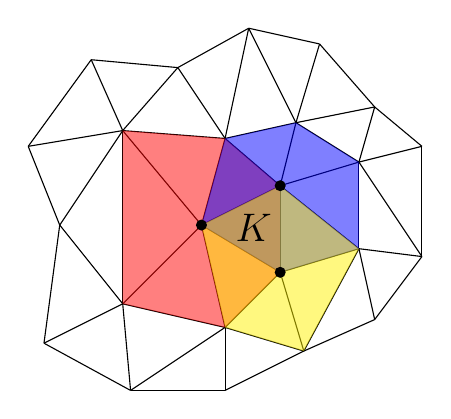
\begin{tikzpicture}[
  scale=1]

\def\pointsize{2pt}

\coordinate (p1) at (1,1);
\coordinate (p2) at (2.1,0.4);
\coordinate (p3) at (3.3,0.4);
\coordinate (p4) at (4.3,0.9);
\coordinate (p5) at (5.2,1.3);
\coordinate (p6) at (5.8,2.1);
\coordinate (p7) at (5.8,3.5);
\coordinate (p8) at (5.2,4);
\coordinate (p9) at (4.5,4.8);
\coordinate (p10) at (3.6,5);
\coordinate (p11) at (2.7,4.5);
\coordinate (p12) at (1.6,4.6);
\coordinate (p13) at (0.8,3.5);
\coordinate (p14) at (1.2,2.5);
\coordinate (p15) at (2,1.5);
\coordinate (p16) at (3.3,1.2);
\coordinate (p17) at (4,1.9);
\coordinate (p18) at (5,2.2);
\coordinate (p19) at (5,3.3);
\coordinate (p20) at (4.2,3.8);
\coordinate (p21) at (3.3,3.6);
\coordinate (p22) at (2,3.7);
\coordinate (i) at (3,2.5);
\coordinate (j) at (4,3);

%\fill (p1) circle (\pointsize);
%\fill (p2) circle (\pointsize);
%\fill (p3) circle (\pointsize);
%\fill (p4) circle (\pointsize);
%\fill (p5) circle (\pointsize);
%\fill (p6) circle (\pointsize);
%\fill (p7) circle (\pointsize);
%\fill (p8) circle (\pointsize);
%\fill (p9) circle (\pointsize);
%\fill (p10) circle (\pointsize);
%\fill (p11) circle (\pointsize);
%\fill (p12) circle (\pointsize);
%\fill (p13) circle (\pointsize);
%\fill (p14) circle (\pointsize);
%\fill (p15) circle (\pointsize);
%\fill (p16) circle (\pointsize);
%\fill (p17) circle (\pointsize);
%\fill (p18) circle (\pointsize);
%\fill (p19) circle (\pointsize);
%\fill (p20) circle (\pointsize);
%\fill (p21) circle (\pointsize);
%\fill (p22) circle (\pointsize);
%\fill (i) circle (\pointsize);
%\fill (j) circle (\pointsize);

\draw (p1) -- (p2);
\draw (p1) -- (p14);
\draw (p1) -- (p15);
\draw (p2) -- (p3);
\draw (p2) -- (p15);
\draw (p2) -- (p16);
\draw (p3) -- (p4);
\draw (p3) -- (p16);
\draw (p4) -- (p5);
\draw (p4) -- (p16);
\draw (p4) -- (p17);
\draw (p4) -- (p18);
\draw (p5) -- (p6);
\draw (p5) -- (p18);
\draw (p6) -- (p7);
\draw (p6) -- (p18);
\draw (p6) -- (p19);
\draw (p7) -- (p8);
\draw (p7) -- (p19);
\draw (p8) -- (p9);
\draw (p8) -- (p19);
\draw (p8) -- (p20);
\draw (p9) -- (p10);
\draw (p9) -- (p20);
\draw (p10) -- (p11);
\draw (p10) -- (p20);
\draw (p10) -- (p21);
\draw (p11) -- (p12);
\draw (p11) -- (p21);
\draw (p11) -- (p22);
\draw (p12) -- (p13);
\draw (p12) -- (p22);
\draw (p13) -- (p14);
\draw (p13) -- (p22);
\draw (p14) -- (p15);
\draw (p14) -- (p22);
\draw (p15) -- (i);
\draw (p15) -- (p16);
\draw (p15) -- (p22);
\draw (p16) -- (i);
\draw (p16) -- (p17);
\draw (p17) -- (i);
\draw (p17) -- (j);
\draw (p17) -- (p18);
\draw (p18) -- (j);
\draw (p18) -- (p19);
\draw (p19) -- (j);
\draw (p19) -- (p20);
\draw (p20) -- (j);
\draw (p20) -- (p21);
\draw (p21) -- (i);
\draw (p21) -- (j);
\draw (p21) -- (p22);
\draw (p22) -- (i);
\draw (i) -- (j);



\draw[draw=none, fill=red, fill opacity=0.5] (p15)--(p16)--(p17)--(j)
  --(p21)--(p22)--cycle;
\draw[draw=none, fill=blue, fill opacity=0.5] (p17)--(p18)--(p19)--(p20)
  --(p21)--(i)--cycle;
\draw[draw=none, fill=yellow, fill opacity=0.5] (p16)--(i)--(j)--(p18)
  --(p4)--cycle;

\node[black] at ($0.333*(i) + 0.333*(j) + 0.333*(p17)$) {\Large $K$};

\fill[black] (i) circle (\pointsize);
\fill[black] (j) circle (\pointsize);
\fill[black] (p17) circle (\pointsize);

\end{tikzpicture}

      \caption{Illustration of Cell Degree of Freedom Indices $\indices_K$}
   \label{fig:cell_indices}
\end{figure}
%-------------------------------------------------------------------------------
This viscosity definition is designed to give the minimum amount of artificial
diffusion without violating the M-matrix conditions.

Now the low-order system will be described.
Consider a modification of the Galerkin scheme given in Equation \eqref{eq:galerkin_semidiscrete}
which lumps the mass matrix ($\M^C \rightarrow \M^L$) and adds an artificial
diffusion operator $\D^L$, hereafter called the low-order diffusion matrix:
\begin{equation}
  \M^L\ddt{\U^L} + (\A + \D^L)\U(t) = \ssrhs(t) \eqc
\end{equation}
where $\U^L(t)$ denotes the discrete low-order solution values.
Defining the low-order steady-state system matrix $\A^L\equiv\A + \D^L$,
the low-order system for the steady-state system, explicit Euler system,
and Theta system, respectively, are
\begin{equation}\label{eq:low_ss}
  \A^L \U = \ssrhs \eqc
\end{equation}
\begin{equation}\label{eq:low_fe}
  \M^L\frac{\U^{n+1} - \U^n}{\dt} + \A^L\U^n = \ssrhs^n \eqc
\end{equation}
\begin{equation}\label{eq:low_theta}
  \M^L\frac{\U^{n+1} - \U^n}{\dt} + \A^L\pr{\theta\U^{n+1} + (1-\theta)\U^n}
    = \ssrhs^\theta \eqc
\end{equation}
where $\ssrhs^\theta \equiv (1-\theta)\ssrhs^n + \theta\ssrhs^{n+1}$.
The low-order
diffusion matrix is assembled element-wise using the local viscous bilinear
form and low-order viscosity definitions:
\begin{equation}\label{eq:low_order_diffusion_matrix}
  D_{i,j}^L \equiv
    \sum\limits_{K\in \mathcal{K}(S_{i,j})}\nu^L_K
    d_K(\test_j,\test_i) \eqp
\end{equation}

Now the low-order scheme has been fully described, and some statements will be
made on its properties. Firstly the M-matrix property will be claimed for
the matrix $\A^L$.
%-------------------------------------------------------------------------------
\begin{thm}[M-matrix property]
  The low-order steady-state system matrix $\A^L$ is a non-singular M-matrix.
\end{thm}
In this section, it will be shown that the low-order steady-state system matrix
defined in Equation \eqref{eq:low_order_ss_matrix} is an M-matrix, which allows
a discrete maximum principle for the low-order solution to be proven in Section
\ref{sec:DMP}.
%--------------------------------------------------------------------------------
\begin{lemma}[lem:offdiagonalnegative]{Non-Positivity of Off-Diagonal Elements}
   The off-diagonal elements of the linear system matrix are non-positive:
   \[
     \ssmatrixletter^{L,\timeindex}\ij\le 0, \quad j\ne i \eqp
   \]
\end{lemma}

\begin{proof}
This proof begins by bounding the term $\diffusionmatrixletter\ij^{L,\timeindex}$:
\begin{eqnarray*}
   \diffusionmatrixletter\ij^{L,\timeindex}=
     \sumKSij\mkern-20mu\lowordercellviscosity[\timeindex]
   \localviscbilinearform{\cell}{j}{i}
   & = & \sumKSij\max\limits_{k\ne \ell\in \indicescell}
     \pr{\frac{\max(0,\ssmatrixletter_{k,\ell}^\timeindex)}
       {\mkern10mu-\mkern-20mu\sum\limits_{T:\celldomain[T]\subset\support_{k,\ell}}
       \mkern-20mu\localviscbilinearform{T}{\ell}{k}}}
     \localviscbilinearform{\cell}{j}{i} \eqp
\end{eqnarray*}
Since $\localviscbilinearform{\cell}{j}{i} < 0$ for $j\ne i$ and $y_i \leq
\max_j y_j$,
\begin{eqnarray*}
   \diffusionmatrixletter\ij^{L,\timeindex} & \le &
     \sumKSij \frac{\max(0,\ssmatrixletter\ij^\timeindex)}
   {\mkern10mu-\mkern-20mu\sumKSij[T]\mkern-20mu\localviscbilinearform{T}{j}{i}}
   \localviscbilinearform{\cell}{j}{i} \eqc\\
   &  =  & -\max(0,\ssmatrixletter\ij^\timeindex)
     \frac{\sumKSij\mkern-20mu\localviscbilinearform{\cell}{j}{i}}
     {\sumKSij[T]\mkern-20mu\localviscbilinearform{T}{j}{i}} \eqc\\
   &  =  & -\max(0,\ssmatrixletter\ij^\timeindex) \eqc\\
   & \le & -\ssmatrixletter\ij^\timeindex \eqp
\end{eqnarray*}
Applying this inequality to Equation \eqref{eq:low_order_ss_matrix} gives
\begin{eqnarray*}
  \ssmatrixletter^{L,\timeindex}\ij &  =  &
    \ssmatrixletter\ij^\timeindex + \diffusionmatrixletter\ij^{L,\timeindex}
    \eqc\\
  \ssmatrixletter^{L,\timeindex}\ij & \le &
    \ssmatrixletter\ij^\timeindex - \ssmatrixletter\ij^\timeindex
    \eqc\\
  \ssmatrixletter^{L,\timeindex}\ij & \le & 0 \eqp \qed
\end{eqnarray*}
\end{proof}
%--------------------------------------------------------------------------------
\begin{lemma}[lem:diagonalpositive]{Non-Negativity of Diagonal Elements}
   The diagonal elements  of the linear system matrix are non-negative:
   \[
     \ssmatrixletter^{L,\timeindex}_{i,i}\ge 0 \eqp
   \]
\end{lemma}

\begin{proof}
The diagonal elements of the low-order system matrix are
\[
  \ssmatrixletter^{L,\timeindex}_{i,i} =
    \intSi\mathbf{\consfluxletter}'(\approximatescalarsolution^\timeindex)\cdot
    \nabla\testfunction_i(\x)\testfunction_i(\x)d\volume
  + \intSi\sigma(\x)\testfunction_i^2(\x)d\volume
  + \sumKSi\mkern-15mu\lowordercellviscosity[\timeindex]
    \localviscbilinearform{\cell}{i}{i}
  \eqp
\]
To prove that $\ssmatrixletter^{L,\timeindex}_{i,i}$ is non-negative, it is sufficient to
prove that each term in the above expression is non-negative. The
non-negativity of the interaction term and viscous term are obvious
($\reactioncoef \ge 0, \, \lowordercellviscosity[\timeindex]\ge 0, \,
\localviscbilinearform{\cell}{i}{i}>0$), but the non-negativity of the divergence
term is not necessarily obvious. On the interior of the domain, the divergence
term gives zero contribution because the divergence integral may be transformed
into a surface integral
$\intSi\mathbf{\consfluxletter}'(\approximatescalarsolution^\timeindex)
\cdot\normalvector\frac{\testfunction_i^2}{2} d\area$ via the
divergence theorem; one can then recognize that the basis function
$\testfunction_i$ evaluates to zero on the boundary of its support
$\support_i$. On the outflow boundary of the domain, the term
$\mathbf{\consfluxletter}'(\approximatescalarsolution^\timeindex)
\cdot\normalvector \frac{\testfunction_i^2}{2}$ is positive because
$\mathbf{\consfluxletter}'(\approximatescalarsolution^\timeindex)
\cdot\normalvector > 0$ for an outflow boundary. This quantity is of
course negative for the inflow boundary, so one must consider the boundary
conditions applied for incoming boundary nodes to determine if this condition
is true and a discrete maximum principle applies. For instance, if a Dirichlet boundary condition is
applied, then a discrete maximum principle does not apply.
strongly imposed on the incoming boundary, so for degrees of freedom $i$ on the
incoming boundary, $\ssmatrixletter^{L,\timeindex}_{i,i}$ will be set equal to some positive
value such as 1 with a corresponding incoming value accounted for in the right
hand side $\ssrhs$ of the linear system.\qed
\end{proof}
%--------------------------------------------------------------------------------
\begin{lemma}{Non-Negativity of Row Sums}
   The sum of all elements in a row $i$ is non-negative:
   \[
     \sumj \ssmatrixletter^{L,\timeindex}\ij \ge 0 \eqp
   \]
\end{lemma}

\begin{proof}
Using the fact that $\sumj\testfunction_j(\x)=1$ and
$\sumj \localviscbilinearform{\cell}{j}{i}=0$,
\begin{eqnarray*}
   \sumj \ssmatrixletter^{L,\timeindex}\ij & = & \sumj \intSij
      \left(\mathbf{\consfluxletter}'(\approximatescalarsolution^\timeindex)
        \cdot\nabla\testfunction_j(\x) +
      \reactioncoef(\x)\testfunction_j(\x)\right)\testfunction_i(\x) d\volume +
      \sumj\sumKSij\mkern-20mu\lowordercellviscosity[\timeindex]\localviscbilinearform{\cell}{j}{i}
      \eqc\\
   & = & \intSi\left(
      \mathbf{\consfluxletter}'(\approximatescalarsolution^\timeindex)\cdot
      \nabla\sumj\testfunction_j(\x) +
      \reactioncoef(\x)\sumj\testfunction_j(\x)\right)
      \testfunction_i(\x) d\volume \eqc\\
   \label{eq:rowsum} & = & \intSi\reactioncoef(\x)\testfunction_i(\x) d\volume
     \eqc\\
   &\ge& 0 \eqp \qed
\end{eqnarray*}
\end{proof}
%--------------------------------------------------------------------------------
\begin{lemma}[lem:diagonallydominant]{Diagonal Dominance}
   $\loworderssmatrix[\timeindex]$ is strictly diagonally dominant:
   \[
     \left|\ssmatrixletter^{L,\timeindex}_{i,i}\right|
     \ge \sumjnoti \left|\ssmatrixletter^{L,\timeindex}\ij\right| \eqp
   \]
\end{lemma}
\begin{proof}
Using the inequalities $\sumj \ssmatrixletter^{L,\timeindex}\ij \ge 0$ and
$\ssmatrixletter^{L,\timeindex}\ij\le 0, j\ne i$, it is proven that
$\loworderssmatrix[\timeindex]$ is strictly diagonally dominant:
\begin{eqnarray*}
  \sumj     \ssmatrixletter^{L,\timeindex}\ij       & \ge & 0 \eqc\\
  \sumjnoti \ssmatrixletter^{L,\timeindex}\ij
    + \ssmatrixletter^{L,\timeindex}_{i,i} & \ge & 0 \eqc\\
  \left|\ssmatrixletter^{L,\timeindex}_{i,i}\right| & \ge &
    \sumjnoti -\ssmatrixletter^{L,\timeindex}\ij
    \eqc\\
  \left|\ssmatrixletter^{L,\timeindex}_{i,i}\right| & \ge
    & \sumjnoti \left|\ssmatrixletter^{L,\timeindex}\ij\right| \eqp \qed
\end{eqnarray*}
\end{proof}
%--------------------------------------------------------------------------------
\begin{lemma}{M-Matrix}
  $\loworderssmatrix[\timeindex]$ is an M-Matrix.
\end{lemma}
\begin{proof}
To prove that a matrix is an M-Matrix, it is sufficient to prove that
the following 3 statements are true:
\begin{enumerate}
\item $\ssmatrixletter^{L,\timeindex}\ij\le 0, j\ne i$,
\item $\ssmatrixletter^{L,\timeindex}_{i,i}\ge 0$,
\item $\left|\ssmatrixletter^{L,\timeindex}_{i,i}\right|
      \ge \sumjnoti \left|\ssmatrixletter^{L,\timeindex}\ij\right|$.
\end{enumerate}
These conditions are proven by Lemmas \ref{lem:offdiagonalnegative},
\ref{lem:diagonalpositive}, and \ref{lem:diagonallydominant}, respectively.\qed
\end{proof}
%--------------------------------------------------------------------------------

%-------------------------------------------------------------------------------
Thus it has been proven that the system matrix for the low-order steady-state
system is an M-matrix, and it remains to prove the same for each of the
transient systems. For the explicit Euler/SSPRK systems, the system matrix
is just the lumped mass matrix $\M^L$, which is easily shown to be an M-matrix
since it is a positive, diagonal matrix. For the $\theta$ temporal
discretization, the system matrix is a linear combination of the lumped mass
matrix and the low-order steady-state system matrix; this linear combination
is also an M-matrix since it is a combination of two M-matrices with non-negative
combination coefficients.

To complete the proof of positivity preservation, it remains to show that
the system right-hand-side vectors for each temporal discretization are
non-negative.
%-------------------------------------------------------------------------------
In this section, it will be shown that the low-order scheme for each temporal
discretization preserves non-negativity of the solution, given that a
CFL-like time step size condition is satisfied. This section
builds upon the results of Section \ref{sec:m_matrix}, which proved that the
low-order system matrix $\loworderssmatrix[n]$ is an M-matrix, which to
recall Equation \eqref{eq:m_matrix}, has the property
\[
  \mathbf{A}\mathbf{x} \geq \mathbf{0} \Rightarrow \mathbf{x} \geq \mathbf{0} \eqc
\]
and thus for a linear system $\mathbf{A}\mathbf{x} = \mathbf{b}$,
proof of non-negativity of the right-hand-side vector proves non-negativity
of the solution $\mathbf{x}$. For each temporal discretization, it will be
shown that the system matrix inverted for the corresponding low-order system
is also an M-matrix and that the right-hand-side vector for each system is
non-negative. Thus positivity-preservation of the solution will be proven.
%--------------------------------------------------------------------------------
\begin{theorem}{Non-Negativity of the Steady-State Low-Order Solution}
  The solution of the steady-state low-order system given by Equation
  \eqref{eq:low_ss} is non-negative:
  \[
    \solutionletter^L_i \geq 0 \eqc \quad \forall i\eqp
  \]
\end{theorem}

\begin{proof}
By Theorem \ref{thm:m_matrix}, the system matrix $\loworderssmatrix$ is an
M-matrix, and by assumption in Section \ref{sec:scalar}, the source $\scalarsource$
is non-negative, and thus the steady-state right-hand-side vector entries
$\ssrhsletter_i$ are non-negative. Invoking the M-matrix property
concludes the proof.\qed
\end{proof}
%--------------------------------------------------------------------------------
\begin{theorem}{Non-Negativity Preservation of the Explicit Euler Low-Order Solution}
  If the old solution $\solutionvector^n$ is non-negative and
  the time step size $\dt$ satisfies
\begin{equation}\label{eq:explicit_cfl}
  \timestepsize \leq \frac{\massmatrixletter_{i,i}^{L}}
    {\ssmatrixletter_{i,i}^{L,\timeindex}}
  \eqc\quad\forall i \eqc
\end{equation}
  then the new solution $\solutionvector^{L,n+1}$ of the explicit Euler low-order
  system given by Equation \eqref{eq:low_explicit_euler} is non-negative:
  \[
    \solutionletter^{L,n+1}_i \geq 0 \eqc \quad \forall i\eqp
  \]
\end{theorem}

\begin{proof}
Rearranging Equation \eqref{eq:low_explicit_euler},
\[
  \lumpedmassmatrix\solutionvector^{L,n+1}
    = \dt\ssrhs^n
      + \lumpedmassmatrix\solutionvector^{n}
      + \dt\loworderssmatrix[n]\solutionvector^{n}
  \eqp
\]
Thus the system matrix to invert is the lumped mass matrix, which is
an M-matrix since it is diagonal and positive. The right-hand-side
vector $\mathbf{y}$ of this system has the entries
\[
  y_i
    = \dt\ssrhsletter^n_i
      + \pr{\lumpedmassentry - \dt\ssmatrixletter^{L,n}_{i,i}}
        \solutionletter^n_i
      - \dt\sumjnoti\ssmatrixletter^{L,n}\ij\solutionletter^n_j
  \eqp
\]
It now just remains to prove that these entries are non-negative.
As stated previously, the source function $\scalarsource$ is assumed
to be non-negative and thus the steady-state right-hand-side
vector is non-negative. Due to the time step size assumption
given by Equation \eqref{eq:explicit_cfl} and Lemma \ref{lem:diagonalpositive},
\[
  \lumpedmassentry - \dt\ssmatrixletter^{L,n}_{i,i} \geq 0 \eqc
\]
and by Lemma \ref{lem:offdiagonalnegative}, the off-diagonal
sum term is also non-negative. Thus $y_i$ is a sum of non-negative
terms. Invoking the M-matrix property concludes the proof.\qed
\end{proof}
%--------------------------------------------------------------------------------
\begin{theorem}{Non-Negativity Preservation of the Theta Low-Order Solution}
  If the old solution $\solutionvector^n$ is non-negative and
  the time step size $\dt$ satisfies
\begin{equation}\label{eq:theta_cfl}
   \timestepsize \leq \frac{\massmatrixletter^L_{i,i}}{(1-\theta)
     \ssmatrixletter_{i,i}^{L,\timeindex}}
   \eqc\quad\forall i \eqc
\end{equation}
  then the new solution $\solutionvector^{L,n+1}$ of the Theta low-order
  system given by Equation \eqref{eq:low_theta} is non-negative:
  \[
    \solutionletter^{L,n+1}_i \geq 0 \eqc \quad \forall i\eqp
  \]
\end{theorem}

\begin{proof}
Rearranging Equation \eqref{eq:low_theta},
\[
  \pr{\lumpedmassmatrix+\theta\dt\loworderssmatrix[n+1]}\solutionvector^{L,n+1}
    = \dt\pr{(1-\theta)\ssrhs^n + \theta\ssrhs^{n+1}}
      + \lumpedmassmatrix\solutionvector^{n}
      - (1-\theta)\dt\loworderssmatrix[n]\solutionvector^n
  \eqp
\]
Thus the system matrix to invert is
$\lumpedmassmatrix+\dt\theta\loworderssmatrix[n+1]$, which is
an M-matrix since it is a linear combination of two M-matrices.
The right-hand-side vector $\mathbf{y}$ of this system has the entries
\[
  y_i
    = \dt\pr{(1-\theta)\ssrhsletter^n_i + \theta\ssrhsletter^{n+1}_i}
      + \pr{\lumpedmassentry - (1-\theta)\dt\ssmatrixletter^{L,n}_{i,i}}
        \solutionletter^n_i
      - (1-\theta)\dt\sumjnoti\ssmatrixletter^{L,n}\ij\solutionletter^n_j
  \eqp
\]
It now just remains to prove that these entries are non-negative.
As stated previously, the source function $\scalarsource$ is assumed
to be non-negative and thus the steady-state right-hand-side
vector is non-negative. Due to the time step size assumption
given by Equation \eqref{eq:theta_cfl} and Lemma \ref{lem:diagonalpositive},
\[
  \lumpedmassentry - (1-\theta)\dt\ssmatrixletter^{L,n}_{i,i} \geq 0 \eqc
\]
and by Lemma \ref{lem:offdiagonalnegative}, the off-diagonal
sum term is also non-negative. Thus $y_i$ is a sum of non-negative
terms. Invoking the M-matrix property concludes the proof.\qed
\end{proof}
%--------------------------------------------------------------------------------

%-------------------------------------------------------------------------------

It can also be shown that the described low-order scheme satisfies a local
discrete maximum principle, which is easily shown given the M-matrix property.
One may decide to use these bounds as the imposed bounds in the FCT
algorithm; however, this approach has been found to yield less accurate solutions
than the approach to be outline in Section \ref{sec:fct} and is thus omitted
for brevity.

\subsection{High-Order Scheme\label{sec:high}}
% !TEX root = ../FCT_radiation_paper.tex

This section describes the entropy viscosity method applied to the scalar
conservation law given by Equation \eqref{eq:scalar_model}. Recall that the entropy
viscosity method is to be used as the high-order scheme in the FCT algorithm,
instead of the standard Galerkin method as has been used previously in FCT-FEM schemes;
for Galerkin FCT-FEM examples, see, for instance,
\cite{kuzmin_FCT,moller_2008,lohner,kuzmin_failsafe,kuzmin_closepacking}.
Usage of the entropy viscosity method in the FCT algorithm ensures convergence
to the entropy solution \cite{guermond_secondorder}.

The entropy viscosity method has been applied to a number of PDEs
such as general scalar conservation laws of the form
\begin{equation}\label{eq:scalar_conservation_law}
  \ppt{u} + \nabla\cdot\mathbf{f}(u) = 0 \eqc
\end{equation}
the inviscid Euler equations \cite{guermond_ev,marco_low_mach},
and the two-phase seven-equation fluid model \cite{marco_SEM}. The scalar model studied
in this paper does not fit into the general form given by Equation~\eqref{eq:scalar_conservation_law},
due to
the addition of the reaction term $\sigma u$ and source term $q$. Application
of entropy viscosity method to the transport equation model is novel and it is described below.

Since the weak form of the problem does not have a unique solution, one
must supply additional conditions called \emph{admissibility} conditions or
\emph{entropy} conditions to filter out spurious weak solutions, leaving
only the physical weak solution, often called the entropy solution.
A number of entropy conditions are valid, but usually the most convenient
entropy condition for use in numerical methods takes the form of an
\emph{entropy inequality}, such as the following, which is valid for the
general scalar conservation law given by Equation \eqref{eq:scalar_conservation_law}:
\begin{equation}
  \ppt{\eta(u)} + \nabla\cdot\mathbf{\Psi}(u) \leq 0 \eqc
\end{equation}
which holds for any convex entropy function $\eta(u)$ and associated entropy
flux $\mathbf{\Psi}(u) \equiv \int \eta'(u)\mathbf{f}'(u)du$.
If one can show that this inequality holds for an arbitrary
convex entropy function, then one proves it holds for all convex entropy
functions  \cite{leveque2002,guermond_ev}.
For the scalar PDE considered in this paper, the entropy inequality becomes
the following:
\begin{equation}
  \ppt{\eta(u)} + \nabla\cdot\mathbf{\Psi}(u) + \eta'(u)\sigma u - \eta'(u)q
    \leq 0 \eqp
\end{equation}
One can verify this inequality by multiplying the governing PDE by $\eta'(u)$
and applying reverse chain rule.

The entropy viscosity method enforces the entropy inequality by measuring
local entropy production and dissipating accordingly. In practice, one
defines the entropy residual:
\begin{equation}
  \mathcal{R}(u) \equiv \ppt{\eta(u)} + \nabla\cdot\mathbf{\Psi}(u)
    + \eta'(u)\sigma u - \eta'(u)q \eqc
\end{equation}
which can be viewed as the amount of violation of the entropy inequality.
The entropy viscosity for an element $K$ is then defined to be proportional
to this violation, for example:
\begin{equation}
  \nu^\eta_K = \frac{c_\mathcal{R}\|\mathcal{R}(u_h)\|_{L^\infty(K)}}
    {\hat{\eta}_K}
    \eqc
\end{equation}
where $\hat{\eta}_K$ is a normalization constant with the units of entropy,
$c_\mathcal{R}$ is a proportionality constant that can be modulated for
each problem, and $\|\mathcal{R}(u_h)\|_{L^\infty(K)}$ is the maximum of the
entropy residual on element $K$, which can be approximated as the maximum over
the quadrature points of element $K$.
Designing a universally appropriate normalization constant $\hat{\eta}_K$ remains
a challenge for the entropy viscosity method (see \cite{marco_low_mach}
for an alternate normalization for low-Mach flows).
%; it is likely that each conservation
%law system would benefit from a specialized definition.
The objective of this
normalization coefficient is to prevent the user from needing to make significant
adjustments to the tuning parameter $c_\mathcal{R}$ for different problems.
A definition that produces reasonable results for a large number of problems
is the following:
\begin{equation}
  \hat{\eta}_K \equiv \left\|\eta-\bar{\eta}\right\|_{L^\infty(\domain)} \eqc
\end{equation}
where $\bar{\eta}$ is the average entropy over the entire computational domain.

In addition to the entropy residual, it can
also be beneficial to measure the jump in the gradient of the entropy flux
across cell interfaces.
Note that given the definition of the entropy flux, the gradient of the entropy
flux is $\nabla\mathbf{\Psi}(u)=\nabla\eta(u)\mathbf{f}'(u)$. Then let
$\mathcal{J}_F$ denote the jump of the normal component of the entropy flux
gradient across face $F$:
\begin{equation}
  \mathcal{J}_F \equiv |\mathbf{f}'(u)\cdot\mathbf{n}_F|
    [\![\nabla\eta(u)\cdot\mathbf{n}_F]\!] \eqc
\end{equation}
where the double square brackets denote a jump quantity. Then we define the
maximum jump on a cell:
\begin{equation}
  \mathcal{J}_K \equiv \max\limits_{F\in\mathcal{F}(K)} |\mathcal{J}_F| \eqp
\end{equation}
Finally, putting everything together, one can define the entropy viscosity
for a cell $K$ to be
\begin{equation}
  \nu^\eta_K = \frac{c_\mathcal{R}\|\mathcal{R}(u_h)\|_{L^\infty(K)}
    + c_\mathcal{J}\mathcal{J}_K}{\hat{\eta}_K}
    \eqp
\end{equation}
However, it is known that the low-order viscosity for an element, as computed
in Section \ref{sec:low}, gives enough local artificial diffusion for
regularization; any amount of viscosity larger than this low-order viscosity would be
excessive. Thus, the low-order viscosity for an element is
imposed as the upper bound for the high-order viscosity:
\begin{equation}
  \nu^H_K \equiv \min(\nu^L_K, \nu^\eta_K) \eqp
\end{equation}
One can note that, in smooth regions, this high-order viscosity will be
small, and, in regions of strong gradients or discontinuities,
the entropy viscosity can be relatively large.
%, ideally approximately
%as large as the low-order viscosity. Note that the latter condition can
%be achieved in part by tuning the parameters
%$c_\mathcal{R}$ and $c_\mathcal{J}$ for the particular problem.

Finally, the high-order system of equations for the various time discretizations
are as follows:
\begin{subequations}
Steady-state:
\begin{equation}\label{eq:high_ss}
  \A^H \U = \ssrhs \eqc
\end{equation}
Explicit Euler:
\begin{equation}\label{eq:high_fe}
  \M^C\frac{\U^{n+1} - \U^n}{\dt} + \A^{H,n}\U^n = \ssrhs^n \eqc
\end{equation}
Theta scheme:
\begin{equation}\label{eq:high_theta}
  \M^C\frac{\U^{n+1} - \U^n}{\dt} + \theta\A^{H,n+1}\U^{n+1}
    + (1-\theta)\A^{H,n}\U^n
    = \ssrhs^\theta \eqc
\end{equation}
\end{subequations}
where the high-order steady-state system matrix is defined as
$\A^H\equiv\A + \D^H$, and the high-order diffusion matrix $\D^H$ is defined similarly
to the low-order case but using the high-order viscosity instead of the low-order
viscosity:
\begin{equation}\label{eq:high_order_diffusion_matrix}
  D_{i,j}^H \equiv
    \sum\limits_{K\in \mathcal{K}(S_{i,j})}\nu^H_K
    d_K(\test_j,\test_i) \eqp
\end{equation}
Note that unlike the low-order scheme, the high-order scheme does not lump the
mass matrix.

\begin{rmk}
Note that due to the nonlinearity of the entropy viscosity, the entropy viscosity
scheme is nonlinear for implicit and steady-state temporal discretizations, and
thus some nonlinear solution technique must be utilized. For the results in
this paper, a simple fixed-point iteration scheme is used. An alternative
such as Newton's method is likely to be advantageous in terms of the number
of nonlinear iterations; however, fixed-point is used here for comparison
with the nonlinear FCT scheme to be described in Section \ref{sec:fct}.
\end{rmk}

\subsection{FCT Scheme\label{sec:fct}}
% !TEX root = ../paper.tex

\subsubsection{The FCT System}

The entropy viscosity method described in Section \ref{sec:high} enforces
the entropy condition and thus produces numerical approximations that
converge to the entropy solution. However, numerical solutions may still
contain spurious oscillations and negativities, although these effects are
smaller in magnitude than for the corresponding Galerkin solution.
In this paper, the flux-corrected transport (FCT) algorithm
is used to further mitigate the formation of spurious oscillations and
to guarantee the absence of negativities.

The first ingredient of the FCT algorithm is the definition of the antidiffusive
fluxes. To arrive at this definition, the low-order systems, given by Equations
\eqref{eq:low_ss}, \eqref{eq:low_fe}, and \eqref{eq:low_theta} for each temporal
discretization, are augmented with the addition of the \emph{antidiffusion source}
$\p$, which now, instead of producing the low-order solution, produces the high-order
solution $\mathbf{U}^H$.
\begin{subequations}
\begin{equation}\label{eq:antidiffusionsource_ss}
  \A^L \U^H = \ssrhs + \p \eqc
\end{equation}
\begin{equation}\label{eq:antidiffusionsource_fe}
  \M^L\frac{\U^H - \U^n}{\dt} + \A^L\U^n = \ssrhs^n + \p^n \eqc
\end{equation}
\begin{equation}\label{eq:antidiffusionsource_theta}
  \M^L\frac{\U^H - \U^n}{\dt} + \A^L\pr{\theta\U^{n+1} + (1-\theta)\U^n}
    = \ssrhs^\theta + \p^\theta \eqp
\end{equation}
\end{subequations}
Then the corresponding high-order systems, given by Equations \eqref{eq:high_ss},
\eqref{eq:high_fe}, \eqref{eq:high_theta} are subtracted from these equations
to give the following definitions for $\p$:
\begin{subequations}
\begin{equation}\label{eq:antidiffusionsourcei_ss}
  \p \equiv \pr{\D^L - \D^H}\U^H \eqc
\end{equation}
\begin{equation}\label{eq:antidiffusionsourcei_fe}
  \p^n \equiv -\pr{\M^C - \M^L}\frac{\U^H - \U^n}{\dt} + \pr{\D^L - \D^H}\U^n \eqc
\end{equation}
\begin{multline}\label{eq:antidiffusionsourcei_theta}
  \p^\theta \equiv -\pr{\M^C - \M^L}\frac{\U^H - \U^n}{\dt}
    + (1-\theta)\pr{\D^L - \D^{H,n}}\U^n\\
    + \theta    \pr{\D^L - \D^{H,n+1}}\U^{n+1} \eqc
\end{multline}
\end{subequations}
The next step is to decompose each antidiffusive source $p_i$ into a sum of
antidiffusive fluxes: $p_i = \sum_j P_{i,j}$. Because the matrices $\M^C-\M^L$
and $\D^L-\D^H$ are symmetric and feature row sums of zero, the following
are valid antidiffusive flux decompositions:
\begin{subequations}
\begin{equation}
  P_{i,j} = \pr{D^L_{i,j} - D^H_{i,j}}\pr{U^H_j - U^H_i} \eqc
\end{equation}
\begin{equation}
  P^n_{i,j} = -M^C_{i,j}\pr{\frac{U^H_j - U^n_j}{\dt} - \frac{U^H_i - U^n_i}{\dt}}
    + \pr{D^L_{i,j} - D^{H,n}_{i,j}}\pr{U^n_j - U^n_i}  \eqc
\end{equation}
\begin{multline}
  P^{\theta}_{i,j} = -M^C_{i,j}\pr{\frac{U^H_j - U^n_j}{\dt} - \frac{U^H_i - U^n_i}{\dt}}
    + (1-\theta)\pr{D^L_{i,j} - D^{H,n}_{i,j}}\pr{U^n_j - U^n_i}\\
    + \theta\pr{D^L_{i,j} - D^{H,n+1}_{i,j}}\pr{U^H_j - U^H_i} \eqp
\end{multline}
\end{subequations}
Note that this decomposition yields equal and opposite antidiffusive flux pairs
since the antidiffusion matrix $\P$ is skew symmetric: $P_{j,i}=-P_{i,j}$
(and likewise for $P_{j,i}^n$ and $P_{j,i}^\theta$).
Up until this point, no changes have been made to the
high-order scheme: solving Equations \eqref{eq:antidiffusionsource_ss} through
\eqref{eq:antidiffusionsource_theta} still produces the high-order solution.
FCT is applied to these equations by applying limiting coefficients $L_{i,j}$ to
each antidiffusive flux $P_{i,j}$. Thus the FCT systems are the following:
\begin{subequations}
\begin{equation}\label{eq:fct_ss}
  \A^L \U^H = \ssrhs + \hat{\p} \eqc
\end{equation}
\begin{equation}\label{eq:fct_fe}
  \M^L\frac{\U^H - \U^n}{\dt} + \A^L\U^n = \ssrhs^n + \hat{\p}^n \eqc
\end{equation}
\begin{equation}\label{eq:fct_theta}
  \M^L\frac{\U^H - \U^n}{\dt} + \A^L\pr{\theta\U^{n+1} + (1-\theta)\U^n}
    = \ssrhs^\theta + \hat{\p}^\theta \eqc
\end{equation}
\end{subequations}
where the hat denotes limitation: $\hat{p}_i\equiv\sum_j L_{i,j}P_{i,j}$.
The limiting coefficients range between zero and one, representing
full limitation and no limitation, respectively.
For example, setting all limiting
coefficients to zero would result in the low-order solution, and setting
all to one would result in the high-order solution. The actual values of the
limiting coefficients are determined by the limiter, which operates on the
following goal: maximize the limiting coefficients such that the imposed
solution bounds are not violated.

As will be discussed in Section \ref{sec:solution_bounds}, the solution bounds
for implicit FCT and steady-state FCT are implicit, and thus the systems given
by Equations \eqref{eq:fct_theta} and \eqref{eq:fct_ss} are nonlinear, since
the limiting coefficients contained in $\hat{\p}$ are nonlinear.
In this paper, a fixed-point iteration scheme is used to resolved the nonlinearities.
For any nonlinear iteration scheme, the
imposed solution bounds must be computed using the previous solution iterate:
\begin{equation}
  U_i^{-,(\ell)} \leq U_i^{(\ell+1)} \leq U_i^{+,(\ell)} \eqp
\end{equation}
Though the solution bounds are lagged, the antidiffusion bounds $\hat{p}_i^\pm$
still contains terms at iteration $\ell+1$; these terms must be lagged as well.
As a consequence, the solution bounds for implicit/steady-state
FCT schemes are only satisfied upon nonlinear convergence, not at each iteration.

%===============================================================================
% !TEX root = ../FCT_radiation_paper.tex

\subsubsection{Solution Bounds}\label{sec:solution_bounds}

The integral form of the transport equation can be derived using the method
of characteristics. Consider a frame of reference moving with the radiation field so that position is a function of time, resulting in a family of characteristic curves
(since the transport equation is linear, these curves are straight lines)
$\x(t)$ that solve the following ODE:
\begin{equation}
  \ddt{\x}=v\di\eqc \quad \x(0)=\x_0\eqp
\end{equation}
Then taking the time derivative of $u(\x(t),t)$ gives
\begin{align}
  \ddt{u} & = \ppt{u} + \nabla\cdot(u(\x(t),t))\ddt{\x}\\
    & =  \ppt{u} + \nabla\cdot(u(\x(t),t))\ddt{\x}
\end{align}
Finally, combining this with Equation \eqref{eq:scalar_model} and solving
the resulting ODE gives the integral transport equation \cite{glasstone}:
\begin{multline}\label{eq:integral_transport}
   u(\x,t) = u_0(\x - v t\di) e^{-\int\limits_0^t
    \sigma(\x - v(t -t')\di)v dt'}\\
    + \int\limits_0^t q(\x - v(t -t')\di,t') e^{-\int\limits_{t'}^t
    \sigma(\x - v(t -{t''})\di)v d{t''}} v dt' \eqp
\end{multline}

% %================================================================================
% \section{Introduction}
% %================================================================================
% In this section, an analytic local maximum principle is derived for
% scalar conservation laws having a constant, linear flux $\consfluxscalar$,
% i.e., $\consfluxscalar = \velocity u$ with $\nabla\cdot(\velocity u) =
% \velocity\cdot\nabla u$, where $\velocity$ is the constant velocity field. This
% analysis is valid for radiation transport, where the constant velocity field is
% $\velocity=v\directionvector$, with $v$ being the radiation speed.
%
% The analytic DMPs are derived using the method of characteristics, whereby
% paths in the $x-t$ plane are found, along which the governing PDE becomes an ODE.
% This is simple for the case of constant linear transport because in this case
% the characteristics are constant.
%
% %================================================================================
% \section{Integral Form of the Linear Transport Equation}
% %================================================================================
% \begin{theorem}{Integral Form of the Linear Transport Equation}{}
%    An implicit solution to the initial value problem
%    \begin{equation}\label{PDE}
%      \frac{1}{v}\ppt{\scalarsolution}
%        + \directionvector\cdot\nabla\scalarsolution(\x,t)
%         + \sigma(\x)\scalarsolution(\x,t)
%         = q(\x,t),
%      \qquad \scalarsolution(\x,0) = \scalarsolution_0(\x)
%    \end{equation}
%    is the following:
%    \begin{equation}\label{eq:integral_form}
%       \scalarsolution(\x,t) = \scalarsolution_0(\x - v t\directionvector)
%          e^{-\int\limits_0^t \sigma(\x - v(t -t')\directionvector)v dt'} +
%          \int\limits_0^t q(\x - v(t -t')\directionvector,t')
%            e^{-\int\limits_{t'}^t\sigma(\x
%              - v(t -\bar{t})\directionvector)v d\bar{t}} v dt' \eqp
%    \end{equation}
% \end{theorem}
%
% \begin{proof}
%    This proof will proceed by using the method of characteristics. The position
%    $\x$ will be regarded as a function of time: $\x=\x(t)$.
%    The characteristic $\x(t)$ is the solution of the following initial value problem:
%    \[
%       \frac{d\x}{dt} = v\directionvector \eqc \qquad \x(0) = \x_0 \eqc
%    \]
%    which is
%    \[
%       \x(t) = \x_0 + v t\directionvector \eqp
%    \]
%    Taking the derivative of $\scalarsolution(\x(t),t)$ gives
%    \begin{eqnarray*}
%       \frac{d\scalarsolution}{dt} & = &\ppt{\scalarsolution}
%         + \nabla\cdot\scalarsolution(\x(t),t) \frac{d\x}{dt}\\
%         & = & \ppt{\scalarsolution}
%         + v\directionvector\cdot\nabla\scalarsolution(\x(t),t) \eqc
%    \end{eqnarray*}
%    which when combined with the PDE in Equation \eqref{PDE}, gives
%    \begin{equation}\label{eq:pre_integrating_factor}
%       \ddt{\scalarsolution} + v\sigma(\x(t))\scalarsolution(\x(t),t)
%         = vq(\x(t),t) \eqp
%    \end{equation}
%    This is a 1st-order linear ODE, which may be solved using an integrating factor
%    \[
%       \mu(t)=e^{\int\limits_0^t\sigma(\x(t'))v dt'}.
%    \]
%    Multiplying both sides of Equation \eqref{eq:pre_integrating_factor}
%    by this integrating factor and using the product rule,
%    \[
%       \frac{d}{dt}\left[\scalarsolution(\x(t),t)\mu(t)\right]
%         = vq(\x(t),t) \mu(t) \eqc
%    \]
%    and integrating from $0$ to $t$ gives
%    \[
%       \scalarsolution(\x(t),t)\mu(t)-\scalarsolution(\x(0),0)\mu(0) =
%          \int\limits_0^t q(\x(t'),t') \mu(t') v dt' \eqp
%    \]
%    Simplifying,
%    \[\begin{split}
%       \scalarsolution(\x(t),t) &= \scalarsolution(\x(0),0)
%          e^{-\int\limits_0^t \sigma(\x(t'))v dt'} +
%          \left(\int\limits_0^t q(\x(t'),t')
%            e^{\int\limits_0^{t'}\sigma(\x(\bar{t}))v d\bar{t}}
%            v dt'\right)
%          e^{-\int\limits_0^tv\sigma(\x(t'))dt'} \eqc\\
%       &= \scalarsolution(\x(0),0)
%          e^{-\int\limits_0^t \sigma(\x(t'))v dt'} +
%          \int\limits_0^t q(\x(t'),t')
%            e^{-\int\limits_{t'}^t\sigma(\x(\bar{t}))v d\bar{t}}
%            v dt' \eqp
%    \end{split}\]
%    Finally, expressing $\x(t)$ in terms of $\x$, $v$, $\directionvector$,
%    and $t$ gives
%    \begin{multline*}
%       \scalarsolution(\x,t) = \scalarsolution_0(\x - v t\directionvector)
%          e^{-\int\limits_0^t \sigma(\x - v(t -t')\directionvector)
%            v dt'}\\
%          + \int\limits_0^t q(\x - v(t -t')\directionvector,t')
%            e^{-\int\limits_{t'}^t\sigma(\x
%              - v(t -\bar{t})\directionvector)v d\bar{t}}
%              v dt'\eqp \qed
%    \end{multline*}
% \end{proof}
% %================================================================================
% \section{Local Maximum Principles\label{sec:local_max_principles}}
% %================================================================================
% Before giving an analytic local discrete maximum principle, a local maximum
% principle applying to a general region is given by the following theorem.
%
% \begin{theorem}[thm:analytic_max_principle]{Analytic Local Maximum Principle}
%    Let $L(\x,\tau)$ be the line segment that spans between
%    $\x-v\tau\directionvector$ and $\x$:
%    \begin{equation}
%       L(\x,\tau)\equiv \left\{\mathbf{y}\in\mathbb{R}^d : \mathbf{y}
%          = \x-v t\directionvector \eqc \qquad t\in(0,\tau) \right\} \eqp
%    \end{equation}
%    See Figure \ref{fig:neighborhood} for an illustration.
%    The following local maximum principle is valid for the solution to the
%    problem given by Equation \eqref{PDE}:
%    \begin{subequations}\label{eq:local_max_principle}
%    \begin{equation}
%       \scalarsolution_{\text{min}} \le \scalarsolution(\x,\tau)
%         \le \scalarsolution_{\text{max}} \eqc
%    \end{equation}
%    \begin{equation}
%       \scalarsolution_{\text{min}}
%         \equiv \left\{\begin{array}{l l}
%           %\scalarsolution_{\min,N}^0
%           \scalarsolution_0(\x - v \tau\directionvector)
%              e^{-v\tau\sigma_{\max,L}}
%             + \frac{q_{\min,L}}{\sigma_{\max,L}}
%              (1 - e^{-v\tau\sigma_{\max,L}}) \eqc
%           & \sigma_{\max,L} \ne 0 \\
%           %\scalarsolution_{\min,L}^0
%           \scalarsolution_0(\x - v \tau\directionvector)
%             + v\tauq_{\min,L} \eqc
%           & \sigma_{\max,L} = 0
%         \end{array}\right.\eqc
%    \end{equation}
%    \begin{equation}
%       \scalarsolution_{\text{max}}
%         \equiv \left\{\begin{array}{l l}
%           %\scalarsolution_{\max,N}^0
%           \scalarsolution_0(\x - v \tau\directionvector)
%             e^{-v\tau\sigma_{\min,L}}
%             + \frac{q_{\max,L}}{\sigma_{\min,L}}
%             (1 - e^{-v\tau\sigma_{\min,L}}) \eqc
%           & \sigma_{\min,L} \ne 0 \\
%           %\scalarsolution_{\max,N}^0
%           \scalarsolution_0(\x - v \tau\directionvector)
%             + v\tauq_{\max,L} \eqc
%           & \sigma_{\min,L} = 0
%         \end{array}\right.\eqc
%    \end{equation}
%    \begin{equation}
%      \sigma_{\min,L}\equiv\min\limits_{\mathbf{y}\in L(\x,\tau)}
%        \sigma(\mathbf{y}) \eqc \quad
%      \sigma_{\max,L}\equiv\max\limits_{\mathbf{y}\in L(\x,\tau)}
%        \sigma(\mathbf{y}) \eqc
%    \end{equation}
%    \begin{equation}
%      q_{\min,L}\equiv\min\limits_{\mathbf{y}\in L(\x,\tau)}
%        q(\mathbf{y}) \eqc \quad
%      q_{\max,L}\equiv\max\limits_{\mathbf{y}\in L(\x,\tau)}
%        q(\mathbf{y}) \eqp
%    \end{equation}
%    \end{subequations}
% \end{theorem}
% %-------------------------------------------------------------------------------
% \begin{figure}[htb]
%    \centering
%      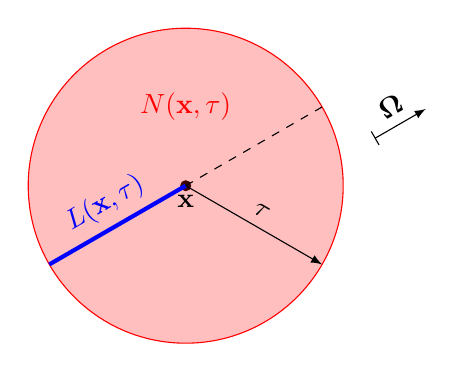
\begin{tikzpicture}[
  scale=1]

\def\pointsize{2pt}
\def\radius{2}

\coordinate (mycenter) at (0,0);
\fill (mycenter) circle (\pointsize);
\draw[draw=red, fill=red, fill opacity=0.25] (mycenter) circle (\radius);
\draw (mycenter) node[below] {$\x$};
\draw[-latex] (mycenter) -- (-30:\radius) node[pos=0.5,sloped,above] {$\speed\tau$};
\draw[blue,line width=1.5pt] (mycenter) -- (210:\radius)
  node[pos=0.5,sloped,above] {$L(\x,\tau)$};
\draw[dashed] (mycenter) -- (30:\radius);
\node[red] at ($0.5*(0,\radius)$) {$N(\x,\tau)$};
\coordinate (dircenter) at (1.2*\radius,0.3*\radius);
\draw[|-latex,shift=(dircenter)] (0,0) -- (30:0.75)
  node[pos=0.5,sloped,above] {$\di$};

\end{tikzpicture}

%       \caption{Illustration of Neighborhoods $L(\x,\tau)$ and $N(\x,\tau)$}
%    \label{fig:neighborhood}
% \end{figure}
% %-------------------------------------------------------------------------------
% \begin{proof}
%    Rewriting Equation \eqref{eq:integral_form} with $t=\tau$ gives
%    \begin{multline*}
%       \scalarsolution(\x,\tau) = \scalarsolution_0(\x - v\tau\directionvector)
%          e^{-\int\limits_0^\tau \sigma(\x
%            - v(\tau -t')\directionvector)v dt'}\\
%          +
%          \int\limits_0^\tau q(\x - v(\tau -t')\directionvector,t')
%          e^{-\int\limits_{t'}^\tau \sigma(\x
%          - v(\tau -\bar{t})\directionvector)v d\bar{t}}v dt' \eqp
%    \end{multline*}
%    One can bound the first term in the right-hand-side of Equation
%    \eqref{eq:integral_form} by considering
%    the maximum and minimum cross section on the line segment $L(\x,\tau)$
%    for the lower and upper bounds, respectively:
%    \[
%       %\scalarsolution_{\min,L}^0
%       \scalarsolution_0(\x - v\tau\directionvector)
%         e^{-v\tau\sigma_{\max,L}} \le
%       \scalarsolution_0(\x - v\tau\directionvector)
%         e^{-\int\limits_0^\tau \sigma(\x
%            - v(\tau -t')\directionvector)v dt'} \le
%       %\scalarsolution_{\max,L}^0
%       \scalarsolution_0(\x - v\tau\directionvector)
%         e^{-v\tau\sigma_{\min,L}} \eqp
%    \]
%    The source term can be bounded as follows:
%    \begin{align*}
%      \scalarsolution_q
%       & \equiv
%          \int\limits_0^\tau q(\x - v(\tau -t')\directionvector,t')
%          e^{-\int\limits_{t'}^\tau \sigma(\x
%            - v(\tau -\bar{t})\directionvector)v d\bar{t}} v dt'\\
%       & \le
%          q_{\max,L}\int\limits_0^\tau
%          e^{-\int\limits_{t'}^\tau \sigma(\x
%            - v(\tau -\bar{t})\directionvector)v d\bar{t}}v dt'\\
%       & \le
%          q_{\max,L}\int\limits_0^\tau
%          e^{-\sigma_{\min,L}\int\limits_{t'}^\tau v d\bar{t}}v dt'\\
%       & =
%          q_{\max,L} \int\limits_0^\tau
%          e^{-v(\tau-t')\sigma_{\min,L}}v dt'\\
%       & =
%          q_{\max,L}e^{-v\tau\sigma_{\min,L}}
%          \int\limits_0^\tau e^{\sigma_{\min,L}v t'}v dt'\\
%       & =
%          \left\{\begin{array}{l l}
%             \frac{q_{\max,L}}{\sigma_{\min,L}}
%               (1 - e^{-v\tau\sigma_{\min,L}}) \eqc
%                & \sigma_{\min,L} \ne 0\\
%             v\tau q_{\max,L} \eqc & \sigma_{\min,L} = 0
%             \end{array}\right.
%    \end{align*}
%    A similar analysis is performed for the lower bound.
%    Putting the two components together gives the bounds given by Equation
%    \eqref{eq:local_max_principle}.\qed
% \end{proof}
% %-------------------------------------------------------------------------------
%
% This result gives relatively tight solution bounds; however, its use as
% solution bounds for FCT may prove difficult in practice (especially for
% multi-dimensional problems), as one must
% compute the solution at the point $\x-v\tau\di$ and must be able
% to evaluate the minimum and maximum of the reaction coefficients and
% sources on the line segment $L(\x_i,\tau)$.
% The following corollary loosens the solution bounds for use in a
% more simple implementation of solution bounds for FCT. It considers
% not just the upstream line segment of length $v\tau$, but the
% sphere of radius $v\tau$ centered at $\x_i$.
%
% %-------------------------------------------------------------------------------
% \begin{corollary}[cly:loose_analytic_max_principle]
%   {Loose Analytic Local Maximum Principle}
% Let $N(\x,\tau)$ denote the sphere centered at $\x$ with radius
% $v\tau$, as shown in Figure \ref{fig:neighborhood}:
%    \begin{equation}\label{eq:neighborhood}
%       N(\x,\tau)\equiv\left\{\mathbf{y}\in\mathbb{R}^d :
%          \|\mathbf{y} - \x\| \le v\tau\right\} \eqp
%    \end{equation}
% The following, looser, local maximum principle is valid for the solution to the
% problem given by Equation \eqref{PDE}:
% \begin{subequations}\label{eq:loose_local_max_principle}
%    \begin{equation}
%       \scalarsolution_{\text{min}} \le \scalarsolution(\x,\tau)
%         \le \scalarsolution_{\text{max}} \eqc
%    \end{equation}
%    \begin{equation}
%       \scalarsolution_{\text{min}}
%         \equiv \left\{\begin{array}{l l}
%           \scalarsolution_{\min,N}^0 e^{-v\tau\sigma_{\max,N}}
%             + \frac{q_{\min,N}}{\sigma_{\max,N}}
%              (1 - e^{-v\tau\sigma_{\max,N}}) \eqc
%           & \sigma_{\max,N} \ne 0 \\
%           \scalarsolution_{\min,N}^0
%             + v\tauq_{\min,N} \eqc
%           & \sigma_{\max,N} = 0
%         \end{array}\right.\eqc
%    \end{equation}
%    \begin{equation}
%       \scalarsolution_{\text{max}}
%         \equiv \left\{\begin{array}{l l}
%           \scalarsolution_{\max,N}^0 e^{-v\tau\sigma_{\min,N}}
%             + \frac{q_{\max,N}}{\sigma_{\min,N}}
%             (1 - e^{-v\tau\sigma_{\min,N}}) \eqc
%           & \sigma_{\min,N} \ne 0 \\
%           \scalarsolution_{\max,N}^0
%             + v\tauq_{\max,N} \eqc
%           & \sigma_{\min,N} = 0
%         \end{array}\right.\eqc
%    \end{equation}
%    \begin{equation}
%      \scalarsolution_{\min,N}^0 \equiv \min\limits_{\mathbf{y}\in N(\x,\tau)}
%        \scalarsolution(\mathbf{y},0) \eqc \quad
%      \scalarsolution_{\max,N}^0 \equiv \max\limits_{\mathbf{y}\in N(\x,\tau)}
%        \scalarsolution(\mathbf{y},0) \eqc
%    \end{equation}
%    \begin{equation}
%      \sigma_{\min,L}\equiv\min\limits_{\mathbf{y}\in L(\x,\tau)}
%        \sigma(\mathbf{y}) \eqc \quad
%      \sigma_{\max,L}\equiv\max\limits_{\mathbf{y}\in L(\x,\tau)}
%        \sigma(\mathbf{y}) \eqc
%    \end{equation}
%    \begin{equation}
%      q_{\min,L}\equiv\min\limits_{\mathbf{y}\in L(\x,\tau)}
%        q(\mathbf{y}) \eqc \quad
%      q_{\max,L}\equiv\max\limits_{\mathbf{y}\in L(\x,\tau)}
%        q(\mathbf{y}) \eqp
%    \end{equation}
% \end{subequations}
% \end{corollary}
% %-------------------------------------------------------------------------------
% \begin{proof}
% Because $\x-v\tau\di\in N(\x,\tau)$,
% \[
%   \scalarsolution_0(\x - v\tau\directionvector) \geq \scalarsolution_{\min,N}^0
%   \eqc \quad
%   \scalarsolution_0(\x - v\tau\directionvector) \leq \scalarsolution_{\max,N}^0
%   \eqp
% \]
% Because $L(\x,\tau)\subset N(\x,\tau)$ (see Figure \ref{fig:neighborhood}),
% the following is true:
% \[
%   q_{\min,N} \leq q_{\min,L}
%   \eqc \quad
%   q_{\max,N} \geq q_{\max,L}
%   \eqc
% \]
% \[
%   \sigma_{\min,N} \leq \sigma_{\min,L}
%   \eqc \quad
%   \sigma_{\max,N} \geq \sigma_{\max,L}
%   \eqp
% \]
% Applying these inequalities to Equation \eqref{eq:local_max_principle}
% proves Equation \eqref{eq:loose_local_max_principle}.\qed
% \end{proof}
% %-------------------------------------------------------------------------------
%
% The following theorem applies Corollary \ref{cly:loose_analytic_max_principle} to derive
% an analytic discrete maximum principle for radiation transport.
%
% %-------------------------------------------------------------------------------
% \begin{theorem}[thm:analytic_dmp]{Analytic Discrete Maximum Principle}
\noindent
If the time step size $\dt$ satisfies the condition
\begin{equation}\label{eq:cfl_analytic_dmp}
  v\dt \leq h_{\min} \eqc \quad h_{\min} \equiv \min\limits_K h_K \eqc
\end{equation}
where $h_K$ is the diameter of cell $K$, then the following discrete
solution bounds apply:
\begin{subequations}\label{eq:solution_bounds}
  \begin{equation}
      U^-_i \le U_i^{n+1} \le U^+_i \eqc
  \end{equation}
where
  \begin{equation}
      U^-_i
        \equiv \left\{\begin{array}{l l}
          U_{\min,i}^n e^{-v\dt\sigma_{\max,i}}
            + \frac{q_{\min,i}}{\sigma_{\max,i}}
            (1 - e^{-v\dt\sigma_{\max,i}}) \eqc
          & \sigma_{\max,i} \ne 0 \\
          U_{\min,i}^n
            + v\dt q_{\min,i} \eqc
          & \sigma_{\max,i} = 0
        \end{array}\right.\eqc
  \end{equation}
and
  \begin{equation}
      U^+_i
        \equiv \left\{\begin{array}{l l}
          U_{\max,i}^n e^{-v\dt\sigma_{\min,i}}
            + \frac{q_{\max,i}}{\sigma_{\min,i}}
            (1 - e^{-v\dt\sigma_{\min,i}}) \eqc
          & \sigma_{\min,i} \ne 0 \\
          U_{\max,i}^n
            + v\dt q_{\max,i} \eqc
          & \sigma_{\min,i} = 0
        \end{array}\right.\eqp
  \end{equation}
The other quantities used in the above expressions are:
  \begin{equation}
    U_{\max,i}^n \equiv\max\limits_{j\in\indices(S_i)}U_j^n \eqc \quad
    U_{\min,i}^n \equiv\min\limits_{j\in\indices(S_i)}U_j^n \eqc
  \end{equation}
  \begin{equation}
    \sigma_{\max,i} \equiv\max\limits_{\x\in S_i}\sigma(\x) \eqc \quad
    \sigma_{\min,i} \equiv\min\limits_{\x\in S_i}\sigma(\x) \eqc
  \end{equation}
  \begin{equation}
    q_{\max,i} \equiv\max\limits_{\x\in S_i}q(\x) \eqc \quad
    q_{\min,i} \equiv\min\limits_{\x\in S_i}q(\x) \eqp
  \end{equation}
\end{subequations}
Note the time step size condition given by Equation \eqref{eq:cfl_analytic_dmp}
implies that when using CFL numbers greater than 1 with implicit time
discretizations, these bounds no longer apply. Similar bounds can be derived
for $v\dt > h_{min}$; however, these bounds for a node $i$ will no longer
only depend on the solution values of the immediate neighbors of $i$; instead, a larger neighborhood
must be used in the bounds, making the local solution bounds wider and thus less
restrictive and arguably less useful in the FCT algorithm. This represents a
significant disadvantage for implicit FCT, not only because the converged
FCT solution could contain more undesirable features but also because the wider
bounds typically result in a greater number of nonlinear iterations because
of the increased freedom in the limiting coefficients.

Steady-state FCT solution bounds can be inferred from Equation \eqref{eq:solution_bounds}
by making the substitution $v\dt\rightarrow s$, where $0\leq s \leq h_{min}$. This
restriction of $s$ similarly ensures that only the nearest neighbors of $i$ are
needed for the solution bounds of $i$. Steady-state FCT unfortunately suffers
many of the same drawbacks as implicit FCT because like implicit FCT, its
solution bounds are implicit and thus change with each iteration.
% \end{theorem}
% \begin{proof}
% Due to the CFL condition, Equation \eqref{eq:cfl_analytic_dmp}, the support of
% test function $i$ is a superset of the neighborhood $N(\x_i)$ defined by
% Equation \eqref{eq:neighborhood}: $N(\x_i)\subsetS_i$. Thus
% for an arbitrary function of space $f(\x)$,
% \[
%   \max\limits_{\x\in S_i}f(\x)
%     \geq \max\limits_{\x\in N(\x_i)}f(\x) \eqc \quad
%   \min\limits_{\x\in S_i}f(\x)
%     \leq \min\limits_{\x\in N(\x_i)}f(\x) \eqc
% \]
% and
% \[
%   \approximatescalarsolution_{\max,S_i}
%     \geq \approximatescalarsolution_{\max,N} \eqc \quad
%   \approximatescalarsolution_{\min,S_i}
%     \leq \approximatescalarsolution_{\min,N} \eqp
% \]
% Since $\approximatescalarsolution$ is a convex combination of nodal solution
% values, the local extremum are obtained only at nodal values:
% \[
%   \approximatescalarsolution_{\max,S_i}
%     = U_{\max,i} \eqc \quad
%   \approximatescalarsolution_{\min,S_i}
%     = U_{\min,i} \eqp \qed
% \]
% \end{proof}
% %-------------------------------------------------------------------------------
%
% The following corollary extends the analytic discrete maximum principle given
% in Theorem \ref{thm:analytic_dmp} to the steady-state case and is given
% without proof, as it follows the same logic as Theorem \ref{thm:analytic_dmp}.
%
% %-------------------------------------------------------------------------------
% \begin{corollary}{Analytic Steady-State Discrete Maximum Principle}
% If one uses a parameter $s$ such that $s \leq \celldiameter_{\min}$, where
% $\celldiameter_{\min}$ is defined by Equation \eqref{eq:cfl_analytic_dmp}, then
% the following analytic discrete maximum principle bounds apply to the
% steady-state problem:
% \begin{subequations}\label{eq:analyticDMP_ss}
%   \begin{equation}
%       U^-_i \le U_i
%         \le U^+_i \eqc
%   \end{equation}
%   \begin{equation}
%       U^-_i
%         \equiv \left\{\begin{array}{l l}
%           U_{\min,i} e^{-s\sigma_{\max,i}}
%             + \frac{q_{\min,i}}{\sigma_{\max,i}}
%             (1 - e^{-s\sigma_{\max,i}}) \eqc
%           & \sigma_{\max,i} \ne 0 \\
%           U_{\min,i}
%             + sq_{\min,i} \eqc
%           & \sigma_{\max,i} = 0
%         \end{array}\right.\eqc
%   \end{equation}
%   \begin{equation}
%       U^+_i
%         \equiv \left\{\begin{array}{l l}
%           U_{\max,i} e^{-s\sigma_{\min,i}}
%             + \frac{q_{\max,i}}{\sigma_{\min,i}}
%             (1 - e^{-s\sigma_{\min,i}}) \eqc
%           & \sigma_{\min,i} \ne 0 \\
%           U_{\max,i}
%             + sq_{\max,i} \eqc
%           & \sigma_{\min,i} = 0
%         \end{array}\right.\eqp
%   \end{equation}
% \end{subequations}
% \end{corollary}
%
% \begin{remark}
% In practice, one can approximate the maximum/minimum operations
% by taking the maximum/minimum over quadrature points: e.g.,
% $\max\limits_{\x\in S_i} \approx \max\limits_{\x\in Q(S_i)}$,
% where $Q(S_i)$ is the set of quadrature points in $S_i$.
% \end{remark}

%===============================================================================

\subsubsection{Antidiffusion Bounds}

Bounds imposed on a solution value $i$, such as the bounds described in Section
\ref{sec:solution_bounds}, directly translate into bounds on the limited
antidiffusion source $\hat{p}_i$. These antidiffusion bounds $\hat{p}_i^\pm$ for steady-state,
explicit Euler, and Theta discretization are respectively derived by
solving Equations \eqref{eq:fct_ss}, \eqref{eq:fct_fe}, and \eqref{eq:fct_theta}
for $\hat{p}_i$ and manipulating the inequality $U^-_i\leq U_i\leq U^+_i$. This yields:
\begin{subequations}
\begin{equation}\label{eq:antidiffusion_bounds_ss}
  \hat{p}_i^\pm \equiv A_{i,i}^L U_i^\pm
    + \sumjnoti A_{i,j}^L U_j - b_i \eqc
\end{equation}
\begin{equation}\label{eq:antidiffusion_bounds_fe}
  \hat{p}_i^\pm \equiv M^L_{i,i}
    \frac{U_i^\pm - U_i^n}{\dt}
  + \sumj A_{i,j}^L U_j^n
  - b_i^n \eqc
\end{equation}
\begin{equation}\label{eq:antidiffusion_bounds_theta}
  \hat{p}_i^\pm \equiv
   \pr{\frac{M^L_{i,i}}{\dt}+\theta A_{i,i}^L}
     U_i^\pm
    + \pr{(1-\theta) A_{i,i}^L-\frac{M^L_{i,i}}{\dt}}
     U_i^n
  +\sumjnoti A_{i,j}^L U_j^\theta
  -b_i^\theta
  \eqp
\end{equation}
\end{subequations}
We note that, if the limiting coefficients $L_{i,j}$ are selected such that
$\hat{p}_i^-\leq \hat{p}_i\leq \hat{p}_i^+$, then the solution bounds are
satisfied: $U^-_i\leq U_i\leq U^+_i$.

Limiters such as the Zalesak's limiter described in Section \ref{sec:limiter} are algebraic
operator, taking as input the antidiffusion bounds
$\hat{p}_i^\pm$ and the antidiffusive fluxes $P_{i,j}$ and returning as output the
limiting coefficients $L_{i,j}$. It is important to note that most limiters,
including the limiter described in this paper, assume the following:
$\hat{p}_i^-\leq 0$, $\hat{p}_i^+\geq 0$; the reasoning for this assumption
is as follows. Recall that FCT starts from the
low-order scheme, which is equivalent to the solution with $\hat{p}_i=0$.
The limiter should start from this point so that there is a fail-safe solution
for the FCT algoritm: the low-order solution. Otherwise, there is no guarantee
that any combination of values of limiting coefficients will achieve
the desired condition $\hat{p}_i^-\leq \hat{p}_i\leq \hat{p}_i^+$. If
$\hat{p}_i^- > 0$ or $\hat{p}_i^+ < 0$, then the starting state, the low-order
solution, with $\hat{p}_i=0$ is an invalid solution of the FCT algorithm.
Some solution bounds automatically satisfy $\hat{p}_i^-\leq 0$ and $\hat{p}_i^+\geq 0$,
but in general these conditions must be enforced. In this paper, the solution
bounds are possibly widened by directly enforcing these assumptions:
\begin{equation}
  \hat{p}_i^- \gets \min(0,\hat{p}_i^-) \eqc
\end{equation}
\begin{equation}
  \hat{p}_i^+ \gets \max(0,\hat{p}_i^+) \eqp
\end{equation}
Omission of this step can lead to poor results: the assumptions of the
limiter are violated, and thus limiting coefficients that do not satisfy the
imposed solution bounds can be generated. Even negative limiting coefficients
may be generated, and this is especially consequential in implicit FCT
simulations, since the limiting coefficients are then essentially unbounded
toward $-\infty$; iteration can lead to extremely non-physical solutions
and severe convergence difficulties or failure. \tcr{does the last sentence refer to the case when this step is omitted or not?}

%===============================================================================
%--------------------------------------------------------------------------------
\subsection{Limiting Coefficients}\label{L}
%--------------------------------------------------------------------------------
\begin{theorem}{Discrete Maximum Principle-Satisfying Limiting Coefficients}{}
   Suppose that that a discrete maximum principle $W_i^+\le U_i^{n+1}\le W_i^-$
   corresponds to the following inequality for the limited correction fluxes:
   \begin{equation}
      Q_i^- \le \sumj L\ij F\ij \le Q_i^+,
   \end{equation}
   where $Q_i^\pm$ are bounds that depend on the temporal discretization. Then,
   the following limiter coefficient definitions satisfy the discrete maximum
   principle:
   \begin{equation}\label{P_defs}
      P_i^+ \equiv \sum\limits_j\max(0,F_{i,j}) \qquad
      P_i^- \equiv \sum\limits_j\min(0,F_{i,j}),
   \end{equation}
   \begin{equation}\label{R_defs}
      R_i^\pm \equiv\left\{
         \begin{array}{l l}
            1                                          & P_i^\pm = 0\\
            \min\left(1,\frac{Q_i^\pm}{P_i^\pm}\right) & P_i^\pm \ne 0
         \end{array}
         \right.,
   \end{equation}
   \begin{equation}\label{L_defs}
      L_{i,j} \equiv\left\{
         \begin{array}{l l}
            \min(R_i^+,R_j^-) & F_{i,j} \geq 0\\
            \min(R_i^-,R_j^+) & F_{i,j} < 0
         \end{array}
         \right..
   \end{equation}  
\end{theorem}

\begin{proof}
   First, note some properties of the above definitions:
   \begin{gather*}
      P_i^+ \geq 0, \qquad P_i^- \leq 0,\\
      Q_i^+ \geq 0, \qquad Q_i^- \leq 0,\\
      0 \leq R_i^\pm \leq 1,\\
      0 \leq L\ij \leq 1.
   \end{gather*}
   The proof will be given for the upper bound.
   \[
      \sum\limits_j L_{i,j}F_{i,j}
         \leq \sum\limits_{j:F_{i,j}\geq 0} L_{i,j}F_{i,j}
         = \sum\limits_{j:F_{i,j}\geq 0} \min(R_i^+,R_j^-)F_{i,j}
         \leq \sum\limits_{j:F_{i,j}\geq 0} R_i^+ F_{i,j}
   \]
   For the case $P_i^+ = 0$,
   \[
      \sum\limits_{j:F_{i,j}\geq 0} R_i^+ F_{i,j} = 0 \leq Q_i^+
   \]
   For the case $P_i^+ \ne 0$,
   \[
      \sum\limits_{j:F_{i,j}\geq 0} R_i^+ F_{i,j}
      \leq \sum\limits_{j:F_{i,j}\geq 0}\frac{Q_i^+}{P_i^+} F_{i,j}
      = \frac{Q_i^+}{P_i^+} \sum\limits_{j:F_{i,j}\geq 0} F_{i,j}
      = \frac{Q_i^+}{P_i^+} \sum\limits_{j:F_{i,j}\geq 0} \max(0,F_{i,j})
      = Q_i^+
   \]
   Thus,
   \[
      \sum\limits_j L_{i,j}F_{i,j} \leq Q_i^+
   \]
   The lower bound is proved similarly.
   \qed
\end{proof}

%===============================================================================


\section{Results\label{sec:results}}
\documentclass{article}
\usepackage{graphicx}
\usepackage{subcaption}
\usepackage{booktabs}
% required packages
\usepackage{xcolor}
\usepackage{stmaryrd} % jump brackets: \llbracket, \rrbracket

% create a provideenvironment command
\makeatletter
\def\provideenvironment{\@star@or@long\provide@environment}
\def\provide@environment#1{%
  \@ifundefined{#1}%
    {\def\reserved@a{\newenvironment{#1}}}%
    {\def\reserved@a{\renewenvironment{dummy@environ}}}%
  \reserved@a
}
\def\dummy@environ{}
\makeatother

% directories
\newcommand{\diagramdirectory}{../diagrams}

% general
\newcommand{\x}{\mathbf{x}}
\newcommand{\qpoint}{\x_q}
\newcommand{\timevalue}{t}
\newcommand{\timestepsize}{\Delta\timevalue}
\newcommand{\dt}{\timestepsize}
\newcommand{\timeindex}{n}
\newcommand{\speed}{v}
\newcommand{\velocity}{\mathbf{\speed}}
\newcommand{\velocityx}{u}
\newcommand{\velocityy}{v}
\newcommand{\velocityn}{v_n}
\newcommand{\vx}{\velocityx}
\newcommand{\vy}{\velocityy}
\newcommand{\vn}{\velocityn}

% normal vector
\newcommand{\normalvectorletter}{n}
\newcommand{\normalvector}{\mathbf{\normalvectorletter}}
\newcommand{\normalx}{\normalvectorletter_x}
\newcommand{\normaly}{\normalvectorletter_y}
\newcommand{\nx}{\normalx}
\newcommand{\ny}{\normaly}

\newcommand{\ndimensions}{N_\text{dim}}
\newcommand{\ncomponents}{m}
\newcommand{\ndofs}{N_\text{dof}}
\newcommand{\nnodes}{N_\text{node}}
\newcommand{\dofindex}{j}
\newcommand{\nodeindex}{k}
\newcommand{\componentindex}{k}
\newcommand{\transpose}{^{\text{T}}}

% schemes
\newcommand{\low}{L}
\newcommand{\high}{H}

% solution
\newcommand{\scalarsolution}{u}
\newcommand{\vectorsolution}{\mathbf{\scalarsolution}}
\newcommand{\approximate}[1]{\tilde{#1}}
\newcommand{\approximatescalarsolution}{\approximate{\scalarsolution}}
\newcommand{\approximatevectorsolution}{\approximate{\vectorsolution}}
\newcommand{\solutionletter}{U}
\newcommand{\solutionvector}{\mathbf{\solutionletter}}
\newcommand{\U}{\solutionvector}
\newcommand{\lowordersolution}[1][]{
  \ifthenelse{\equal{#1}{}}{\solutionvector^L}{\solutionvector^{L,#1}}}
\newcommand{\highordersolution}[1][]{
  \ifthenelse{\equal{#1}{}}{\solutionvector^H}{\solutionvector^{H,#1}}}

% math
\newcommand{\triangulation}{\mathcal{K}_h}
\newcommand{\approximationspace}{\mathcal{U}_h}
\newcommand{\approximationspaceinc}{\approximationspace^{\textup{inc}}}
\newcommand{\referenceelementmap}{\Phi}
\newcommand{\qonespace}{\mathbb{Q}_1}

% sets
\newcommand{\faces}{\mathcal{F}}
\newcommand{\quadraturepoints}{\mathcal{Q}}

% domain and FEM
\newcommand{\domain}{\mathcal{D}}
\newcommand{\celldomain}[1][\cell]{\domain_#1}
\newcommand{\facedomain}{\domain}
\newcommand{\domainboundary}{\partial\domain}
\newcommand{\incomingdomainboundary}{\domainboundary^{\textup{inc}}}
\newcommand{\cellindex}{K}
\newcommand{\cell}{K}
\newcommand{\celldiameter}{\Delta x}
\newcommand{\maxcelldiameter}{\Delta x_{\text{max}}}
\newcommand{\volume}{V}
\newcommand{\dvolume}{\,d\x}
\newcommand{\area}{A}
\newcommand{\darea}{\,d\area}
\newcommand{\testfunction}{\varphi}
\newcommand{\vectortestfunctionscalar}{\Phi}
\newcommand{\vectortestfunction}{\mathbf{\vectortestfunctionscalar}}
\newcommand{\support}{S}
\newcommand{\maxdof}{N}
\newcommand{\interpolant}{\Pi}

% local viscous bilinear form
\newcommand{\localvisc}{b}
\newcommand{\localviscbilinearform}[3]{\localvisc_#1(\testfunction_#2, \testfunction_#3)}
\newcommand{\cellvolume}{|\celldomain|}
\newcommand{\cardinality}[1][]{\ifthenelse{\equal{#1}{}}{n_\cell}{n_#1}}
\newcommand{\cardsystem}{\bar{n}}
\newcommand{\indices}{\mathcal{I}}
\newcommand{\cellindices}{\mathcal{K}}
\newcommand{\indicesnode}{\indices^{\text{node}}_\cell}
\newcommand{\indicescell}[1][]{\ifthenelse{\equal{#1}{}}{\indices_\cell}
  {\indices_{#1}}}
\newcommand{\incomingindices}{\indices^{\textup{inc}}}
\newcommand{\notincomingindices}{\indices(\triangulation)\setminus\incomingindices}

% entropy viscosity
\newcommand{\entropy}{\eta}
\newcommand{\entropyflux}{\mathbf{\consfluxletter}^\eta}
\newcommand{\entropyjump}{\mathcal{J}}
\newcommand{\entropyresidual}{\mathcal{R}}
\newcommand{\entropyresidualcoef}{c_\entropyresidual}
\newcommand{\entropyjumpcoef}{c_\entropyjump}
\newcommand{\entropynormalization}{\hat{\entropy}}

% conservation law
\newcommand{\consfluxletter}{f}
\newcommand{\consflux}{\mathbf{\consfluxletter}}
\newcommand{\consfluxsystem}{\mathbf{\MakeUppercase{\consfluxletter}}}
\newcommand{\consfluxscalar}[1][\scalarsolution]{\mathbf{\consfluxletter}(#1)}
\newcommand{\consfluxvector}{\mathbf{\MakeUppercase{\consfluxletter}}}
\newcommand{\consfluxvectory}{\mathbf{G}}
\newcommand{\consfluxvectorn}{\consfluxvector_{n}}
\newcommand{\consfluxinterpolant}{\mathrm{F}}
\newcommand{\conssource}{\mathbf{s}}

% viscosity
\newcommand{\viscosity}{\nu}
\newcommand{\cellviscosity}{\viscosity_\cellindex}
\newcommand{\lowordercellviscosity}[1][]{
  \ifthenelse{\equal{#1}{}}{\cellviscosity^L}
  {\cellviscosity^{L,#1}}}
\newcommand{\highordercellviscosity}[1][]{
  \ifthenelse{\equal{#1}{}}{\cellviscosity^H}
  {\cellviscosity^{H,#1}}}
\newcommand{\entropycellviscosity}[1][]{
  \ifthenelse{\equal{#1}{}}{\cellviscosity^\entropy}
  {\cellviscosity^{\entropy,#1}}}

% viscous fluxes
\newcommand{\viscstring}{\text{visc}}
\newcommand{\viscflux}[1]{\mathbf{\consfluxletter}^{\viscstring,#1}}
\newcommand{\viscconsfluxvector}
  {\mathbf{\MakeUppercase{\consfluxletter}}^\viscstring
  (\vectorsolution,\viscosity)}

% mass matrix
\newcommand{\massmatrixletter}{M}
\newcommand{\massmatrix}{\mathbf{\massmatrixletter}}
\newcommand{\M}{\massmatrix}
\newcommand{\consistentmassmatrix}{\massmatrix^C}
\newcommand{\consistentmassentry}{\massmatrixletter^C_{i,j}}
\newcommand{\lumpedmassmatrix}{\massmatrix^L}
\newcommand{\lumpedmassentry}{\massmatrixletter^L_{i,i}}

% gradient matrix (for conservation law systems)
\newcommand{\gradientmatrixletter}{c}
\newcommand{\gradientmatrix}{\mathbf{\MakeUppercase{\gradientmatrixletter}}}
\newcommand{\gradiententry}{\mathbf{\gradientmatrixletter}\ij}

% steady-state system matrix and rhs
\newcommand{\ssmatrixletter}{A}
\newcommand{\ssmatrix}[1][]{
  \ifthenelse{\equal{#1}{}}
  {\mathbf{\ssmatrixletter}}
  {\mathbf{\ssmatrixletter}^#1}}
\newcommand{\A}{\ssmatrix}
\newcommand{\loworderssmatrix}[1][]{
  \ifthenelse{\equal{#1}{}}
  {\ssmatrix^L}
  {\ssmatrix^{L,#1}}}
\newcommand{\highorderssmatrix}[1][]{
  \ifthenelse{\equal{#1}{}}
  {\ssmatrix^H}
  {\ssmatrix^{H,#1}}}
\newcommand{\ssrhsletter}{b}
\newcommand{\ssrhs}[1][]{
  \ifthenelse{\equal{#1}{}}
  {\mathbf{\ssrhsletter}}
  {\mathbf{\ssrhsletter}^#1}}
\renewcommand{\b}{\ssrhs}
\newcommand{\ssresletter}{r}
\newcommand{\ssres}{\mathbf{\ssresletter}}
\renewcommand{\r}{\ssres}
\newcommand{\B}{\mathbf{B}}
\newcommand{\s}{\mathbf{s}}

% diffusion matrix
\newcommand{\diffusionmatrixletter}{D}
\newcommand{\diffusionmatrix}[1][]{
  \ifthenelse{\equal{#1}{}}
  {\mathbf{\diffusionmatrixletter}}
  {\mathbf{\diffusionmatrixletter}^#1}}
\newcommand{\D}{\diffusionmatrix}
\newcommand{\loworderdiffusionmatrix}[1][]{
  \ifthenelse{\equal{#1}{}}
  {\diffusionmatrix^L}
  {\diffusionmatrix^{L,#1}}}
\newcommand{\highorderdiffusionmatrix}[1][]{
  \ifthenelse{\equal{#1}{}}
  {\diffusionmatrix^H}
  {\diffusionmatrix^{H,#1}}}

% Runge-Kutta
\newcommand{\RKstagesolution}{\hat{\mathbf{\solutionletter}}}
\newcommand{\RKintermediatesolution}{\tilde{\mathbf{\solutionletter}}}
\newcommand{\RKoldsolutioncoef}{\alpha}
\newcommand{\RKstagesolutioncoef}{\beta}
\newcommand{\RKtimecoef}{c}
\newcommand{\RKstagetime}{\hat{\timevalue}}
\newcommand{\RKnstages}{s}

% FCT
\newcommand{\solutionbound}{W}
\newcommand{\DMPlowerbound}{\solutionbound^{\textup{DMP},-}}
\newcommand{\DMPupperbound}{\solutionbound^{\textup{DMP},+}}
\newcommand{\DMPlowerboundss}{\solutionbound^{\textup{DMP},\textup{ss},-}}
\newcommand{\DMPupperboundss}{\solutionbound^{\textup{DMP},\textup{ss},+}}
\newcommand{\DMPboundsss}{\solutionbound^{\textup{DMP},\textup{ss},\pm}}
\newcommand{\DMPlowerboundee}{\solutionbound^{\textup{DMP},\textup{ee},-}}
\newcommand{\DMPupperboundee}{\solutionbound^{\textup{DMP},\textup{ee},+}}
\newcommand{\DMPboundsee}{\solutionbound^{\textup{DMP},\textup{ee},\pm}}
\newcommand{\DMPlowerboundtheta}{\solutionbound^{\textup{DMP},\textup{theta},-}}
\newcommand{\DMPupperboundtheta}{\solutionbound^{\textup{DMP},\textup{theta},+}}
\newcommand{\DMPboundstheta}{\solutionbound^{\textup{DMP},\textup{theta},\pm}}
\newcommand{\DMPbounds}{\solutionbound^{\textup{DMP},\pm}}
\newcommand{\analyticDMPbounds}{\solutionbound^{\textup{analytic},\pm}}
\newcommand{\analyticDMPupperbound}{\solutionbound^{\textup{analytic},+}}
\newcommand{\analyticDMPlowerbound}{\solutionbound^{\textup{analytic},-}}
\newcommand{\limitedfluxbound}{Q}
\newcommand{\antidiffusionbound}{\limitedfluxbound}
\newcommand{\antidiffusionboundvector}{\mathbf{\limitedfluxbound}}
\newcommand{\antidiffusionlowerboundss}{\antidiffusionbound^{\textup{ss},-}}
\newcommand{\antidiffusionupperboundss}{\antidiffusionbound^{\textup{ss},+}}
\newcommand{\antidiffusionlowerboundee}{\antidiffusionbound^{\textup{ee},-}}
\newcommand{\antidiffusionupperboundee}{\antidiffusionbound^{\textup{ee},+}}
\newcommand{\antidiffusionlowerboundtheta}{\antidiffusionbound^{\textup{theta},-}}
\newcommand{\antidiffusionupperboundtheta}{\antidiffusionbound^{\textup{theta},+}}
\newcommand{\limitedfluxboundsi}{\limitedfluxbound^\pm_i}
\newcommand{\limiterletter}{L}
\newcommand{\limitermatrix}{\mathbf{\limiterletter}}
\newcommand{\correctionfluxletter}{p}
\newcommand{\correctionfluxvector}{\mathbf{\correctionfluxletter}}
\newcommand{\correctionfluxentry}{\MakeUppercase{\correctionfluxletter}}
\newcommand{\correctionfluxij}{\correctionfluxentry_{i,j}}
\newcommand{\correctionfluxji}{\correctionfluxentry_{j,i}}
\newcommand{\correctionfluxmatrix}{\mathbf{\MakeUppercase{\correctionfluxletter}}}
\newcommand{\antidiffusiveflux}{\correctionfluxentry}

% remainder
\newcommand{\correctionfluxremainder}{\Delta\MakeUppercase{\correctionfluxletter}}
\newcommand{\correctionfluxmatrixremainder}{\Delta\correctionfluxmatrix}
\newcommand{\limitedcorrectionfluxmatrixremainder}
  {\bar{\correctionfluxmatrixremainder}}

\newcommand{\limitedcorrectionfluxletter}{\bar{\correctionfluxletter}}
\newcommand{\cumulativecorrectionfluxletter}{\bar{\correctionfluxletter}}
\newcommand{\cumulativecorrectionfluxvector}{\bar{\correctionfluxvector}}
\newcommand{\cumulativecorrectionfluxvectorchange}
  {\Delta\cumulativecorrectionfluxvector}
\newcommand{\correctionfluxsumsi}{\MakeUppercase{\correctionfluxletter}^\pm_i}
\newcommand{\limitedfluxsum}{\limitermatrix\cdot\correctionfluxmatrix}
\newcommand{\limitedfluxsumi}{\sumj\limiterletter\ij
  \MakeUppercase{\correctionfluxletter}\ij}
\newcommand{\F}{\correctionfluxmatrix}
\newcommand{\LF}{\limitermatrix\cdot\correctionfluxmatrix}
\newcommand{\transformationmatrix}{\mathbf{T}}

% radiation transport
\newcommand{\angularflux}{\psi}
\newcommand{\scalarflux}{\phi}
\newcommand{\speedoflight}{c}
\newcommand{\totalcrosssection}{\Sigma_\text{t}}
\newcommand{\reactioncoef}{\sigma}
\newcommand{\directionvector}{\mathbf{\Omega}}
\newcommand{\di}{\directionvector}
\newcommand{\xdet}{(\x,\di,E,t)}
\newcommand{\xet}{(\x,E,t)}
\newcommand{\scalarsource}{q}
\newcommand{\radiationsource}{Q}

% Euler equations
\newcommand{\density}{\rho}
\newcommand{\totalenergy}{E}
\newcommand{\momentum}{\mathbf{m}}
\newcommand{\pressure}{p}
\newcommand{\gasconstant}{\gamma}
\newcommand{\identity}{\mathbf{I}}

% shallow water equations
\newcommand{\height}{h}
\newcommand{\heightmomentumletter}{q}
\newcommand{\heightmomentum}{\mathbf{\heightmomentumletter}}
\newcommand{\heightmomentumx}{\heightmomentumletter_x}
\newcommand{\heightmomentumy}{\heightmomentumletter_y}
\newcommand{\heightmomentumd}{\heightmomentumletter_d}
\newcommand{\dischargex}{\heightmomentumletter}
\newcommand{\bathymetry}{b}
\newcommand{\waterlevel}{w}
\newcommand{\gravity}{g}
\newcommand{\speedofsound}{a}
\newcommand{\froude}{\mathrm{Fr}}

% Riemann solvers
\newcommand{\shockspeed}{S}
\newcommand{\eigenvalue}{\lambda}
\newcommand{\eigenvaluematrix}{\mathbf{\Lambda}}
\newcommand{\eigenvector}{\mathbf{k}}
\newcommand{\eigenvectormatrix}{\mathbf{K}}
\newcommand{\jacobianx}{\mathbf{A}}
\newcommand{\jacobiany}{\mathbf{B}}
\newcommand{\jacobiann}{\jacobianx_{n}}
\newcommand{\characteristicsolution}{\mathbf{w}}
\newcommand{\wavespeed}{\eigenvalue}
\newcommand{\maxwavespeed}[1][]{
  \ifthenelse{\equal{#1}{}}{\wavespeed^{\text{max}}}{\wavespeed^{\text{max},#1}}}
\newcommand{\wavestrength}{\mathcal{W}}

%==============================================================================
% colors
\colorlet{lightBlue}{blue!20!white}
\colorlet{lightGreen}{green!20!white}

% indexing
\renewcommand{\ij}{_{i,j}}
\newcommand{\ji}{_{j,i}}
\newcommand{\kl}{_{k,\ell}}
\newcommand{\lk}{_{\ell,k}}
\newcommand{\nodei}{_{\nodeindex(i)}}
\newcommand{\nodej}{_{\nodeindex(j)}}
\newcommand{\nodeij}{_{\nodeindex(i),\nodeindex(j)}}
\newcommand{\nodeji}{_{\nodeindex(j),\nodeindex(i)}}
\newcommand{\nodequantity}[1]{\underline{#1}}

% sums and integrals
\newcommand{\sumj}{\sum\limits_j}
\newcommand{\sumjnoti}{\sum\limits_{j\ne i}}
\newcommand{\sumKSi}{\sum\limits_{\cell\in\cellindices(\support_i)}}
%\newcommand{\sumKSij}[1][\cell]
%  {\sum\limits_{#1:\celldomain[#1]\subset\support_{i,j}}}
\newcommand{\sumKSij}[1][\cell]
  {\sum\limits_{#1\in\cellindices(\support\ij)}}
\newcommand{\sumallcells}{\sum\limits_{\cell}}
\newcommand{\intdomain}[1]{\int\limits_\domain #1 \,\dvolume}
\newcommand{\intboundary}[1]{\int\limits_{\domainboundary} #1 \,d\area}
\newcommand{\intSi}{\int\limits_{\support_i}}
\newcommand{\intSij}{\int\limits_{\support_{i,j}}}

% math
\newcommand{\ltwonorm}[1]{\left\|#1\right\|_{L^2}} % L-2 norm

% BC
\newcommand{\interior}{^{\text{in}}}
\newcommand{\BC}{^{\text{BC}}}

% common fractions
\newcommand{\half}{\frac{1}{2}}
\newcommand{\fourth}{\frac{1}{4}}

% derivatives
\newcommand{\dd}[2]{\frac{d #1}{d #2}}               % ordinary derivative
\newcommand{\pd}[2]{\frac{\partial #1}{\partial #2}} % partial derivative
\newcommand{\ppt}[1]{\pd{#1}{t}}                     % partial d/dt
\newcommand{\ppx}[1]{\pd{#1}{x}}                     % partial d/dx
\newcommand{\ppy}[1]{\pd{#1}{y}}                     % partial d/dy
\newcommand{\ddt}[1]{\frac{d#1}{dt}}                 % ordinary d/dt

% typesetting
\newcommand{\pr}[1]{\left(#1\right)} % parentheses
\newcommand{\sq}[1]{\left[#1\right]} % square brackets
\newcommand{\jumpbrackets}[1]{\left\llbracket#1\right\rrbracket} % jump brackets
\newcommand{\tab}{\hspace*{0.5cm}}   % tab for verbatim evironments
\newcommand{\eqp}{\,.} % equation period
\newcommand{\eqc}{\,,} % equation comma

% miscellaneous
\newcommand{\xt}{\pr{\x,\timevalue}}
\newcommand{\divergence}{\nabla\cdot}
\newcommand{\unitvector}[1]{\hat{\mathbf{e}}_{#1}}

% command to highlight term in equation
\newcommand{\highlightblue}[1]{
  \colorbox{lightBlue}{$\displaystyle#1$}}
\newcommand{\highlightgreen}[1]{
  \colorbox{lightGreen}{$\displaystyle#1$}}

% QED symbol command
\providecommand{\qed}{\nobreak \ifvmode \relax \else
  \ifdim\lastskip<1.5em \hskip-\lastskip
  \hskip1.5em plus0em minus0.5em \fi \nobreak
  \vrule height0.75em width0.5em depth0.25em\fi}

% math environments
\provideenvironment{proof}[1][Proof]{\begin{trivlist}
\item[\hskip \labelsep {\bfseries #1}]}{\end{trivlist}}
\provideenvironment{example}[1][Example]{\begin{trivlist}
\item[\hskip \labelsep {\bfseries #1}]}{\end{trivlist}}
\newenvironment{remark}[1][Remark]{\begin{trivlist}
\item[\hskip \labelsep {\bfseries #1}]}{\end{trivlist}}

% table environment
% #1 = caption
% #2 = label
% #3 = table format (columns)
% #4 = header row
\newenvironment{mytable}[4]
  {\begin{table}[htb]\caption{#1\label{tab:#2}}\begin{center}
    \begin{tabular}
    {#3}\hline #4\\\hline}
  {\hline\end{tabular}\end{center}\end{table}}

% references commands
%\newcommand{\refsec}[1]{, \S#1}
\newcommand{\refsec}[1]{}

% algorithm shortcuts
\newcommand{\objective}{\phi}
\newcommand{\hmin}{\height_{\text{min}}}
\newcommand{\hmax}{\height_{\text{max}}}
\newcommand{\hlow}{\check{\height}}
\newcommand{\hhigh}{\hat{\height}}
\newcommand{\hrarefaction}{\tilde{\height}_*}
\newcommand{\tol}{\epsilon}
\newcommand{\minwavespeed}{\wavespeed_{\text{min}}}
\newcommand{\lowwavespeedone}{\check{\wavespeed}_1}
\newcommand{\highwavespeedone}{\hat{\wavespeed}_1}
\newcommand{\lowwavespeedtwo}{\check{\wavespeed}_2}
\newcommand{\highwavespeedtwo}{\hat{\wavespeed}_2}
\newcommand{\hinterplow}{\height_d}
\newcommand{\hinterphigh}{\height_u}

% checkboxes
\usepackage{amssymb}
\usepackage{xcolor}
\definecolor{myorangeheavy}{RGB}{255,150,0}
\newcommand{\checked}{
  \makebox[0pt][l]{$\square$}\raisebox{.15ex}
  {\hspace{0.1em}\textcolor{myorangeheavy}{$\checkmark$}}}
\newcommand{\unchecked}{
  \makebox[0pt][l]{$\square$}\hspace{0.9em}}

% highlighting
\newcommand{\hlorange}[1]{\textcolor{myorangeheavy}{#1}}

% invariant domains
\newcommand{\invariantset}{A}
\newcommand{\admissibleset}{\mathcal{A}}
\newcommand{\discreteprocess}{R}
\newcommand{\convexcoefficient}{a}
\newcommand{\convexelement}{\mathbf{b}}

% spaces
\newcommand{\realspace}[1][]{
  \ifthenelse{\equal{#1}{}}{\mathbb{R}}{\mathbb{R}^{#1}}}

% nonlinear solve
\newcommand{\nonlinearmatrix}{\mathbf{B}}
\newcommand{\nonlinearrhs}{\mathbf{s}}
\newcommand{\relaxationparameter}{\alpha}
\newcommand{\nonlineartolerance}{\epsilon}

% algorithm
\usepackage{algpseudocode}
\usepackage{algorithm}
\newcommand{\Break}{\State \textbf{break}}
\newcommand{\Not}{\textbf{not}\,}
\newcommand{\Error}[1]{\State \textbf{error}: #1}

% boundary conditions
\newcommand{\dirichlet}[1]{\tilde{#1}}

\newcommand{\rowsum}[1]{#1\mathbf{1}}

% convergence and error analysis
\newcommand{\order}{\mathcal{O}}
\newcommand{\err}{e}
\newcommand{\dx}{\Delta x}

% tolerance adjustment for line-breaking, to prevent \overfull warnings
\newenvironment{tolerant}[1]{
  \par\tolerance=#1\relax
}{
  \par
}


\setlength{\evensidemargin}{0in}
\setlength{\oddsidemargin}{0in}
\setlength{\topmargin}{0in}
\setlength{\textwidth}{6.5in}

\begin{document}
\section{Test Problem Descriptions}
In this section, the test problem suite is described. These descriptions
include the domain, initial conditions, boundary conditions, and other
physical parameters.
%================================================================================
\subsection{Void-to-Absorber}\label{sec:void_to_absorber}
This problem examines the angular flux travelling in the $+x$ direction,
starting in a void and reaching a strong absorber region.
Table \ref{tab:void_to_absorber} summarizes the test parameters.

\begin{table}[h]\caption{Void-to-Absorber Test Problem Summary}
\label{tab:void_to_absorber}
\centering
\begin{tabular}{l l}\toprule
\emph{Parameter} & \emph{Value}\\\midrule
Domain & $\mathcal{D} = (0,1)^d$\\
Initial Conditions & $u_0(\x)=0$\\
Boundary Conditions & $u(\x,t)=1,\quad \x\in\partial\mathcal{D}^-,\quad t>0,
   \quad\partial\mathcal{D}^-=\{\x\in\partial\mathcal{D}:\mathbf{n}(\x)
   \cdot\mathbf{\Omega}<0\}$\\
Direction & $\mathbf{\Omega} = \mathbf{e}_x$\\
Cross Section & $\sigma(\x)=\left\{\begin{array}{c l}
   10, & \x\in(\frac{1}{2},1)^d\\
   0,  & \mbox{otherwise}\end{array}\right.$\\
Source & $q(\x,t)=0$\\
Speed & $v=1$\\
Exact Solution & $u(\x,t)=\left\{\begin{array}{l l}
   \left\{\begin{array}{l l}
      e^{-10(x-\frac{1}{2})}, & x\ge\frac{1}{2}, y\ge\frac{1}{2}, z\ge\frac{1}{2}\\
      1,                      & \mbox{otherwise}
   \end{array}\right., & x-t<0\\
   0, & \mbox{otherwise}
   \end{array}\right.$ \\
\bottomrule\end{tabular}
\end{table}
%================================================================================
\subsection{Skew Void-to-Absorber}
This problem is a more general case of the test problem described in
Section \ref{sec:void_to_absorber} in which the transport direction is
not necessarily the $+x$ direction but instead is any direction for which
$\Omega_i\ge 0,\forall i$.
Table \ref{tab:void_to_absorber_skew} summarizes the test parameters,
where the definition of $s$ is given below.

\begin{table}[h]\caption{Skew Void-to-Absorber Test Problem Summary}
\label{tab:void_to_absorber_skew}
\centering
\begin{tabular}{l l}\toprule
\emph{Parameter} & \emph{Value}\\\midrule
Domain & $\mathcal{D} = (0,1)^d$\\
Initial Conditions & $u_0(\x)=0$\\
Boundary Conditions & $u(\x,t)=1,\quad \x\in\partial\mathcal{D}^-,\quad t>0,
   \quad\partial\mathcal{D}^-=\{\x\in\partial\mathcal{D}:\mathbf{n}(\x)
   \cdot\mathbf{\Omega}<0\}$\\
Direction & $\mathbf{\Omega} = \left[\frac{1}{\sqrt{2}},\frac{1}{\sqrt{3}},
   \frac{1}{\sqrt{6}}\right]$\\
Cross Section & $\sigma(\x)=\left\{\begin{array}{c l}
   10, & \x\in(\frac{1}{2},1)^d\\
   0,  & \mbox{otherwise}\end{array}\right.$\\
Source & $q(\x,t)=0$\\
Speed & $v=1$\\
Exact Solution & $u(\x,t)=\left\{\begin{array}{l l}
   \left\{\begin{array}{l l}
      e^{-10s}, & x\ge\frac{1}{2}, y\ge\frac{1}{2}, z\ge\frac{1}{2}\\
      1,        & \mbox{otherwise}
   \end{array}\right., & \x-\mathbf{\Omega}t\notin\mathcal{D}\\
   0, & \mbox{otherwise}
   \end{array}\right.$ \\
\bottomrule\end{tabular}
\end{table}

The condition $\x-\mathbf{\Omega}t\notin\mathcal{D}$ is equivalent to the
following condition:
\[
   \x-\mathbf{\Omega}t\notin\mathcal{D} \Rightarrow
   \exists i: x_i-\Omega_i t < 0,
\]
where $i$ denotes a coordinate direction index $x$, $y$, or $z$.
The distance travelled in the absorber region, $s$, is computed
by first determining which plane segment of the absorber region
through which the line $\x-\mathbf{\Omega}t$ passes; the coordinate
direction normal to this plane is denoted by $i$ and the other
two by $j$ and $k$. This is determined as follows:
\[
   i: \frac{x_i-\frac{1}{2}}{\Omega_i} = \min\limits_j\left(
      \frac{x_j-\frac{1}{2}}{\Omega_j}\right).
\]
Then, $s$ is computed as follows:
\[
   s=\sqrt{s_i^2 + s_j^2 + s_k^2}, \quad
   s_i=x_i-\frac{1}{2}, \quad
   s_j=\frac{\Omega_j}{\Omega_i}s_i, \quad
   s_k=\frac{\Omega_k}{\Omega_i}s_i.
\]
%================================================================================
\subsection{Three-Region}\label{sec:three_region}
This is a 1-D problem that consists of a domain with 3 regions of differing
saturation values $\frac{q}{\sigma}$. This is used to test both reaction
terms and source terms.
Table \ref{tab:three_region} summarizes the test parameters.

\begin{table}[h]\caption{Three-Region Test Problem Summary}
\label{tab:three_region}
\centering
\begin{tabular}{l l}\toprule
\emph{Parameter} & \emph{Value}\\\midrule
Domain & $\mathcal{D} = (0,1)$\\
Initial Conditions & $u_0(\x)=0$\\
Boundary Conditions & $u(\x,t)=1,\quad \x\in\partial\mathcal{D}^-,\quad t>0,
   \quad\partial\mathcal{D}^-=\{\x\in\partial\mathcal{D}:\mathbf{n}(\x)
   \cdot\mathbf{\Omega}<0\}$\\
Direction & $\mathbf{\Omega} = \mathbf{e}_x$\\
Cross Section & $\sigma(\x)=\left\{\begin{array}{c l}
   1,  & x \leq 0.3\\
   10, & 0.3 < x \leq 0.6\\
   5,  & x > 0.6
   \end{array}\right.$\\
Source & $q(\x,t)=\left\{\begin{array}{c l}
   1,  & x \leq 0.3\\
   5,  & 0.3 < x \leq 0.6\\
   10, & x > 0.6
   \end{array}\right.$\\
Speed & $v=1$\\
Exact Solution & $u(\x,t)=\left\{\begin{array}{l l}
   \left\{\begin{array}{l l}
      e^{-10(x-\frac{1}{2})}, & x\ge\frac{1}{2}, y\ge\frac{1}{2}, z\ge\frac{1}{2}\\
      1,                      & \mbox{otherwise}
   \end{array}\right., & x-t<0\\
   0, & \mbox{otherwise}
   \end{array}\right.$ \\
\bottomrule\end{tabular}
\end{table}
%================================================================================

In this section, results are presented for the
source-void-to-absorber test problem. This is a 1-D test problem
with zero incoming flux incident on the left boundary,
a constant source in a void in the left half of the
domain, and an absorber with no source in the right half of the
domain. The test problem description is given by Table
\ref{tab:source_void_to_absorber}.

%-------------------------------------------------------------------------------
\begin{table}[htb]\caption{Source-Void-to-Absorber Test Problem Summary}
\label{tab:source_void_to_absorber}
\centering
\begin{tabular}{l l}\toprule
\emph{Parameter} & \emph{Value}\\\midrule
Domain & $\domain = (0,1)$\\
Initial Conditions & $u_0(x)=0$\\
Boundary Conditions & $u(0,t)=0 \eqc \quad t>0$\\
Direction & $\di = \mathbf{e}_x$\\
Cross Section & $\sigma(x)=\left\{\begin{array}{c l}
   0,  & x < \frac{1}{2}\\
   10, & \mbox{otherwise}\end{array}\right.$\\
Source & $q(\x,t)=\left\{\begin{array}{c l}
   1,  & x < \frac{1}{2}\\
   0,  & \mbox{otherwise}\end{array}\right.$\\
Speed & $\speed=1$\\
Exact Solution & $u(x,t)=\left\{\begin{array}{l l}
   \scalarsolution_{\text{ss}}(x), & x-t<0\\
   0, & \mbox{otherwise}
   \end{array}\right.$ \\
   & $\scalarsolution_{\text{ss}}(x) =
       \left\{\begin{array}{l l}
          e^{-10(x-\frac{1}{2})}, & x\ge\frac{1}{2}\\
          1,                      & \mbox{otherwise}
       \end{array}\right.$\\
\bottomrule\end{tabular}
\end{table}
%-------------------------------------------------------------------------------

Figure \ref{fig:source_void_to_absorber}
shows the results for this problem using SSPRK time discretization,
a CFL of 0.5, and 32 cells.
Entropy residual and jump coefficients $\entropyresidualcoef$ and
$\entropyjumpcoef$ are both 1.
Table \ref{tab:source_void_to_absorber_run_parameters} summarizes the
run parameters to generate the results in this section.
Figure \ref{fig:source_void_to_absorber_fine} shows results
for a finer mesh (256 cells) that illustrates the shortcomings of Galerkin-FCT
vs. EV-FCT: Galerkin-FCT does not necessarily converge to the
entropy solution.

%-------------------------------------------------------------------------------
\begin{table}[ht]\caption{Source-Void-to-Absorber Test Problem Run Parameters}
\label{tab:source_void_to_absorber_run_parameters}
\centering
\begin{tabular}{l l}\toprule
\emph{Parameter} & \emph{Value}\\\midrule
Number of Cells & $N_{cell} = 32, 256$\\
End Time & $t = 1$\\
CFL Number & $\nu = 0.5$\\\midrule
Entropy Function & $\entropy(u) = \frac{1}{2}u^2$\\
Entropy Residual Coefficient & $\entropyresidualcoef = 1$\\
Entropy Jump Coefficient & $\entropyjumpcoef = 1$\\
\bottomrule\end{tabular}
\end{table}
%-------------------------------------------------------------------------------
\begin{figure}[ht]
   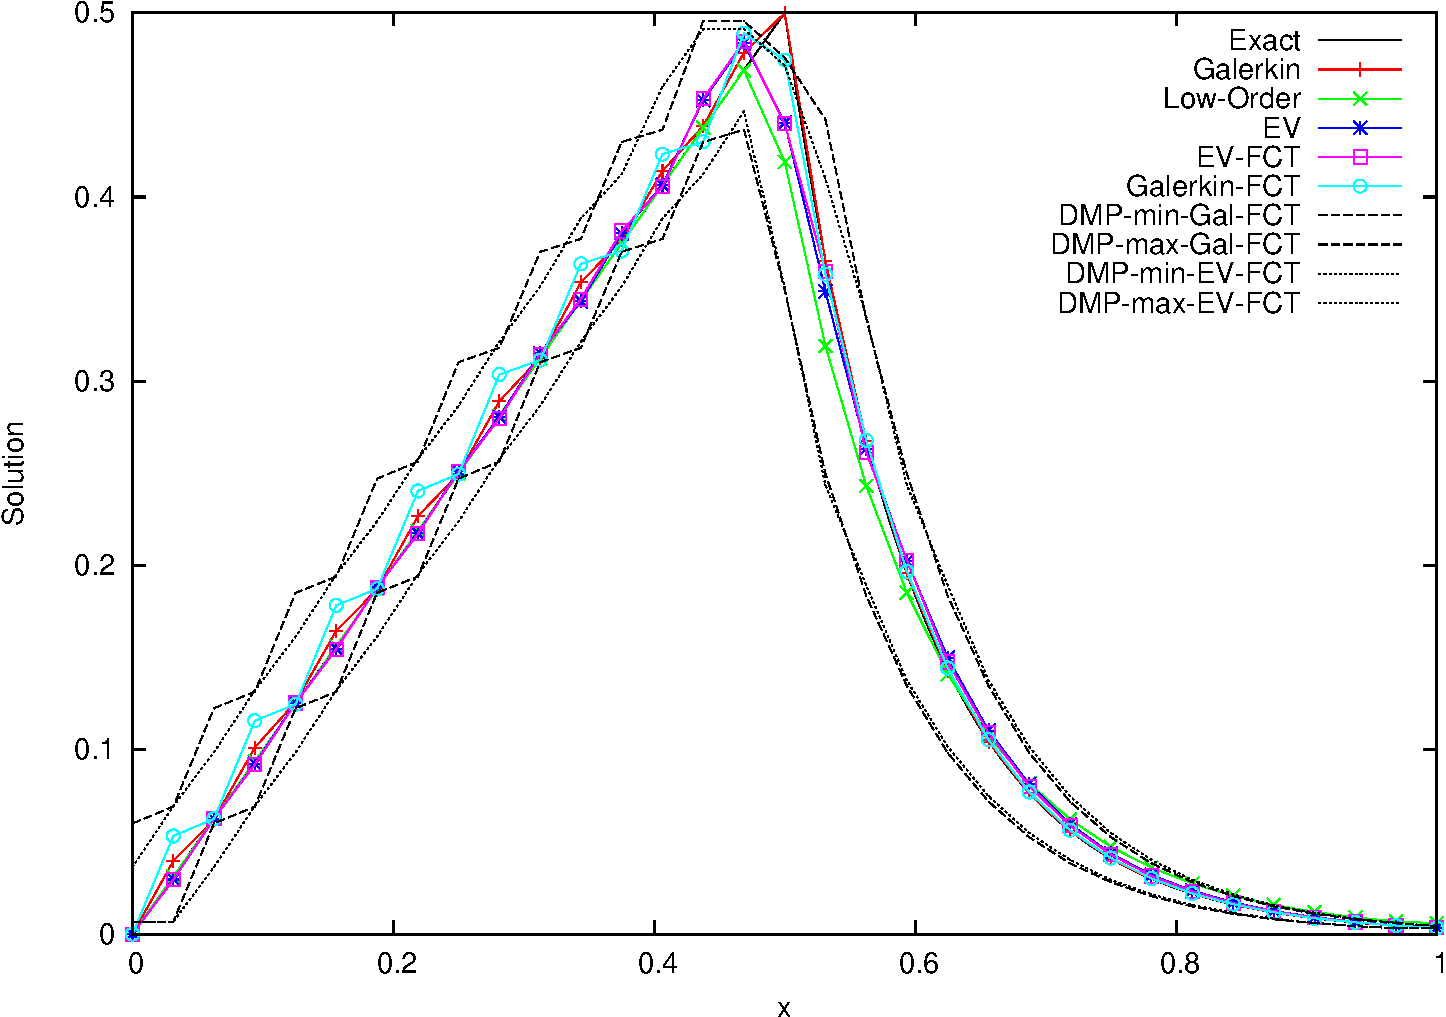
\includegraphics[width=\textwidth]
     {\contentdir/results/transport/source_void_to_absorber/coarse.pdf}
   \caption{Comparison of Solutions for the Source-Void-to-Absorber Problem
     Using SSPRK33 with 32 Cells}
   \label{fig:source_void_to_absorber}
\end{figure}
%-------------------------------------------------------------------------------
\begin{figure}[ht]
   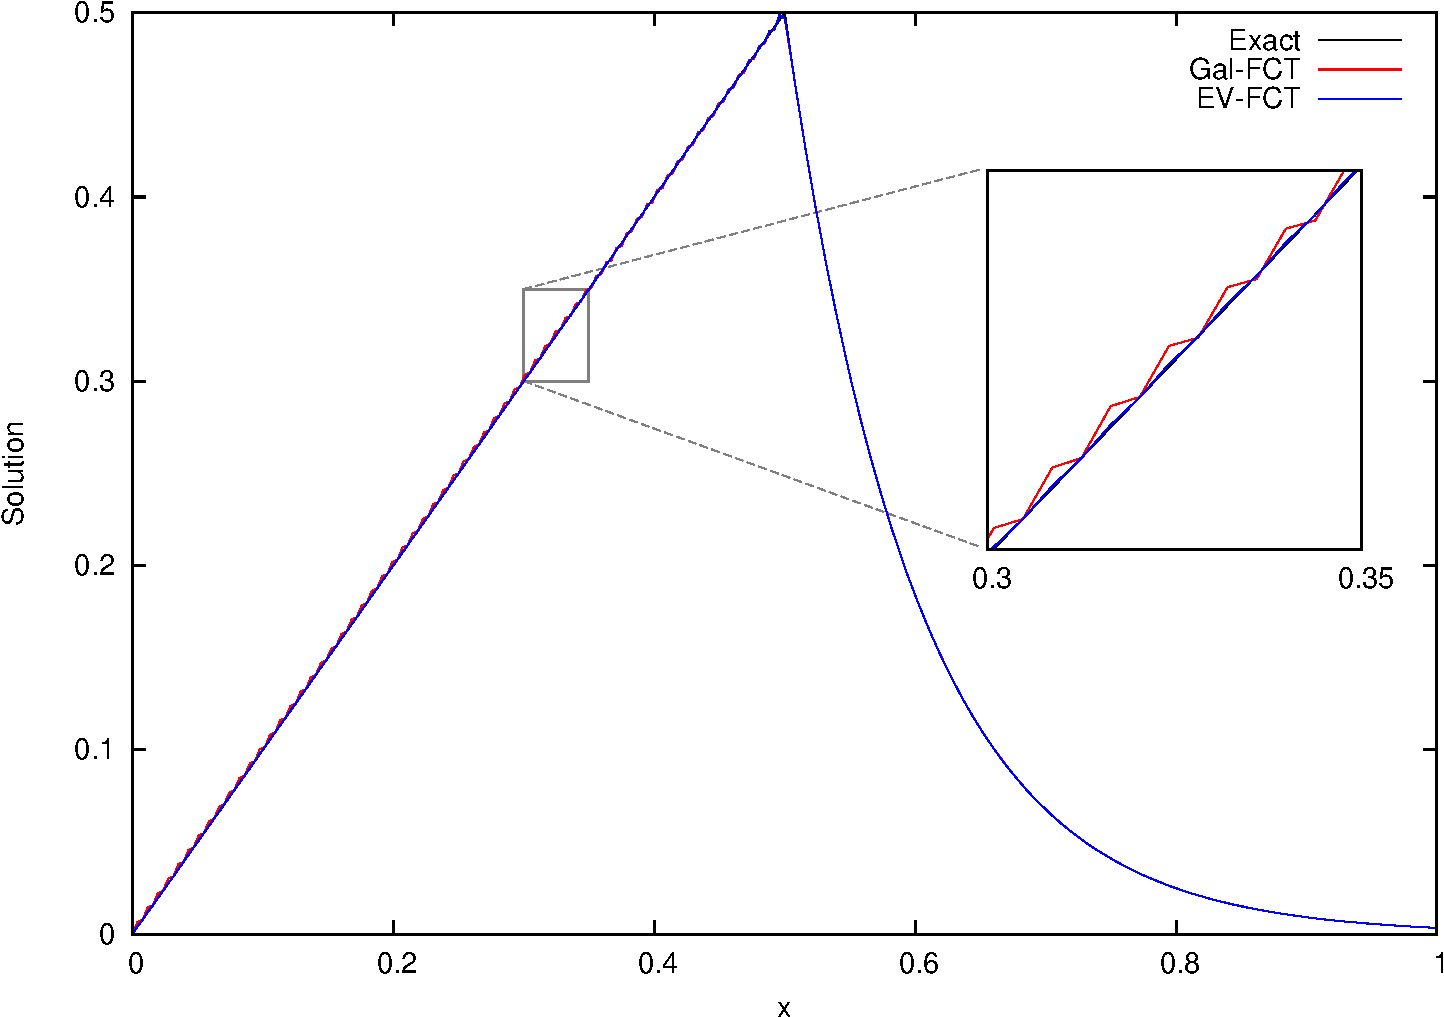
\includegraphics[width=\textwidth]
     {\contentdir/results/transport/source_void_to_absorber/fine.pdf}
   \caption{Comparison of Solutions for the Source-Void-to-Absorber Problem
     Using SSPRK33 with 256 Cells}
   \label{fig:source_void_to_absorber_fine}
\end{figure}
%-------------------------------------------------------------------------------

The steady-state results for this test problem revealed some significant
FCT issues regarding the antidiffusion from Dirichlet nodes.
When Dirichlet boundary conditions are strongly imposed, solution
bounds do not apply, and it becomes unclear how to limit antidiffusion
fluxes from these nodes. Consider symmetric limiters, i.e., those such that
$L\ij=L\ji$, such as Zalesak's limiter, for which
\begin{equation}
  L\ij = \left\{\begin{array}{c c}
    \min(L_i^+,L_j^-) & P\ij > 0\\
    \min(L_i^-,L_j^+) & P\ij < 0\\
  \end{array}\right. \eqp
\end{equation}
Suppose $i$ corresponds to a degree of freedom for which Dirichlet
boundary conditions are strongly imposed. The uncertainty
is the correct way to decide $L_i^+$ and $L_i^-$ since there
are no valid bounds from which to compute these values.
Figures \ref{fig:source_void_to_absorber_strong1} and 
\ref{fig:source_void_to_absorber_strong0} show the solutions obtained
using strongly imposed Dirichlet boundary conditions with these
values set to $L_i^+=L_i^-=1$ and $L_i^+=L_i^-=0$, respectively.
When $L_i^+=L_i^-=1$, the correction flux from the Dirichlet
DoF $i$, which is positive, has only the upper bound for $j$
to consider. The upper bound for $j$, which is inflated above the
analytical solution due to the source, does not restrict this
antidiffusion flux, and thus it is accepted fully to the unphysical
value. Due to the implicitness of the solution bounds, the lower solution
bound for $j$ is computed from this unphysical value and excludes the
possibility of antidiffusion back to the analytical solution. This
process continues with all of the other degrees of freedom.
When instead, $L_i^+=L_i^-=0$, the solution does not lie above
the analytical solution in the source region, but significant peak
clipping appears at the interface between the source and absorber
regions. It should be noted that there are combinations of limiting
coefficient values, each in the range $(0,1)$, that produce a more
accurate solution to this problem (without the peak clipping
and resulting inaccuracy in the absorber region); the problem is that Zalesak's
limiter (and in general, any practical limiter) is not optimal
in the sense that it maximizes the magnitude of antidiffusive flux.
One could in principle solve an optimization problem to select
limiting coefficients that maximize the antidiffusive flux, but this
is very expensive and thus not recommended for general use.

For weakly imposed Dirichlet boundary conditions, solution bounds
still apply, so limiting coefficients may be computed without special
consideration. However, one must now consider the possibility of
inaccurate boundary values.
Figures \ref{fig:source_void_to_absorber_weak} shows the steady-state 
solutions obtained using weakly imposed Dirichlet boundary conditions.
In this case, the antidiffusion flux from the boundary gets limited
(but not fully) due to the lower solution bound of the Dirichlet node.
Because some antidiffusion was accepted here, the peak reaches
a higher value than with the $L_i^+=L_i^-=0$ case.
Finally, Figure \ref{fig:source_void_to_absorber_penalty} shows
the steady-state solution obtained with weakly imposed Dirichlet
boundary conditions and a boundary penalty (see Section \ref{sec:transport_bc}).
The FCT solution looks very similar to the case without any penalty,
but the effect on the low-order and entropy viscosity solutions is
clear.

%-------------------------------------------------------------------------------
\begin{figure}[ht]
   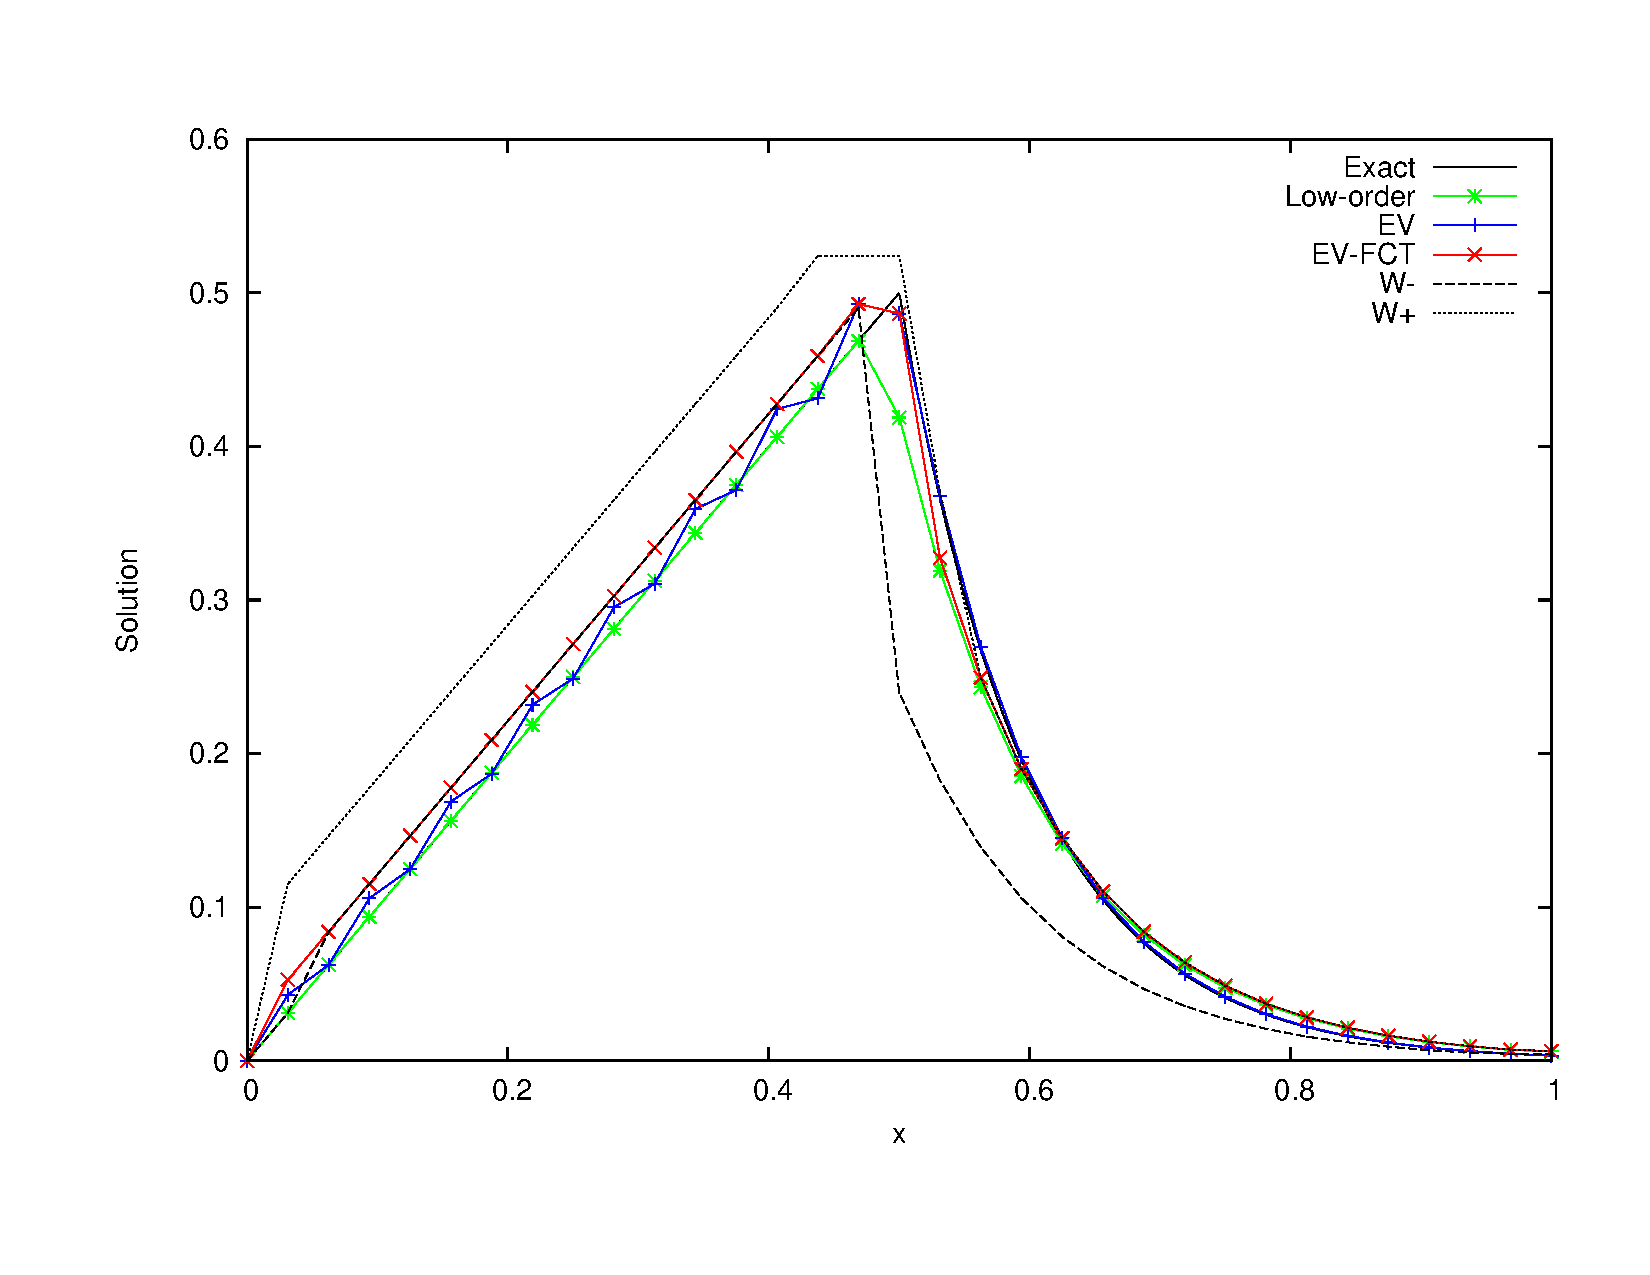
\includegraphics[width=\textwidth]
     {\contentdir/results/transport/source_void_to_absorber/images/strong1.pdf}
   \caption{Steady-State Solutions for the Source-Void-to-Absorber Problem
     with Strongly Imposed Dirichlet Boundary Conditions and $L^-=L^+=1$}
   \label{fig:source_void_to_absorber_strong1}
\end{figure}
%-------------------------------------------------------------------------------
%-------------------------------------------------------------------------------
\begin{figure}[ht]
   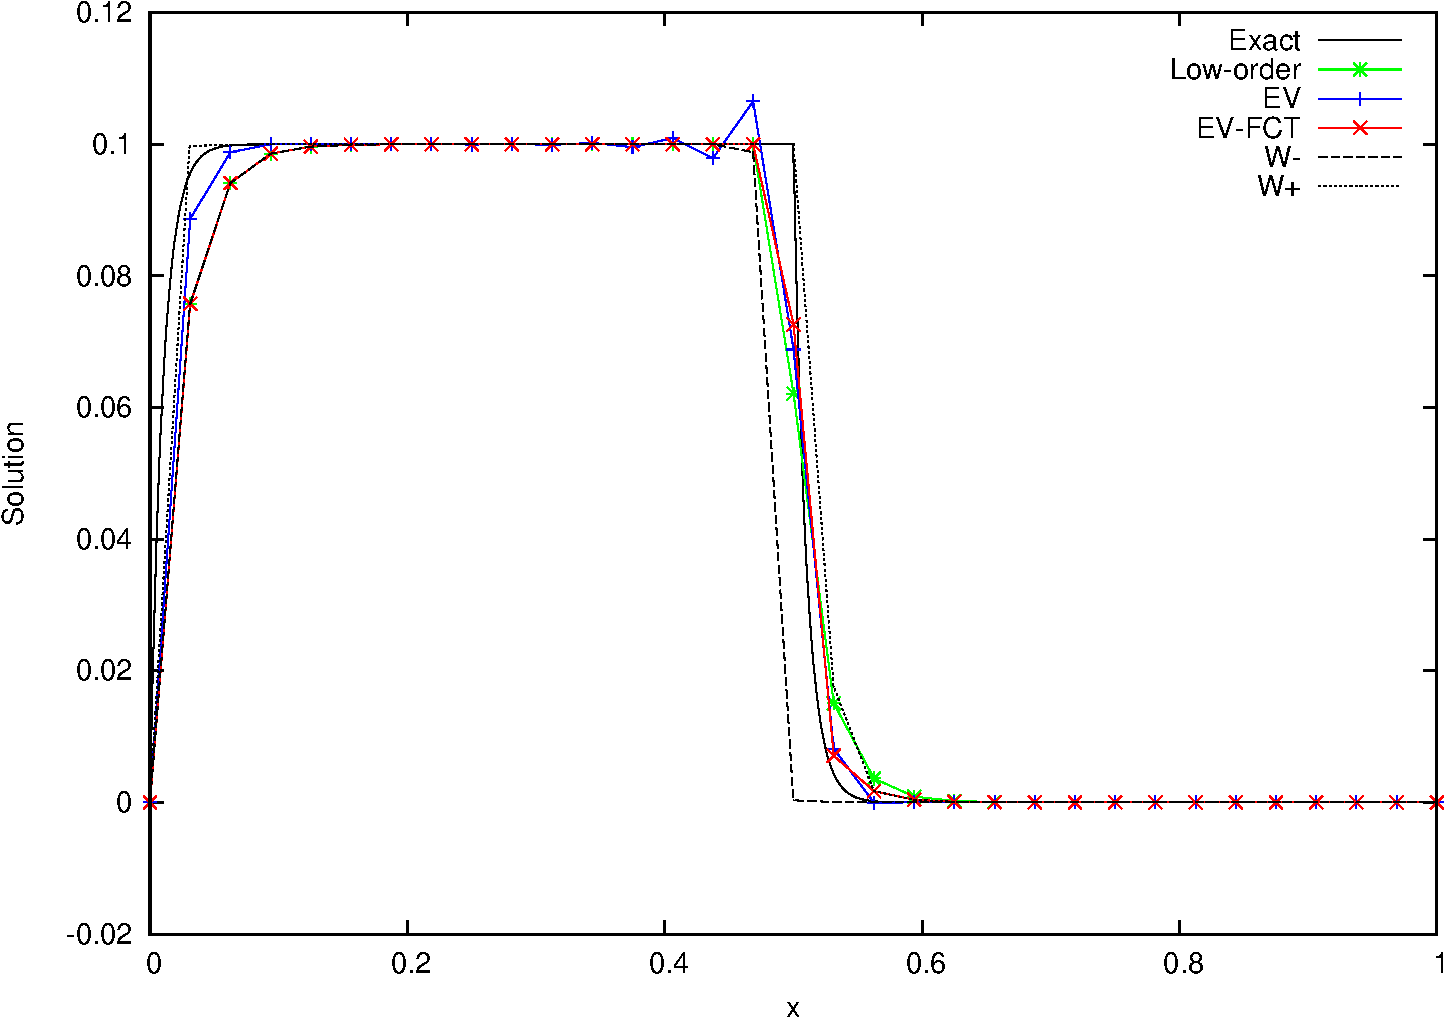
\includegraphics[width=\textwidth]
     {\contentdir/results/transport/source_void_to_absorber/images/strong0.pdf}
   \caption{Steady-State Solutions for the Source-Void-to-Absorber Problem
     with Strongly Imposed Dirichlet Boundary Conditions and $L^-=L^+=0$}
   \label{fig:source_void_to_absorber_strong0}
\end{figure}
%-------------------------------------------------------------------------------
%-------------------------------------------------------------------------------
\begin{figure}[ht]
   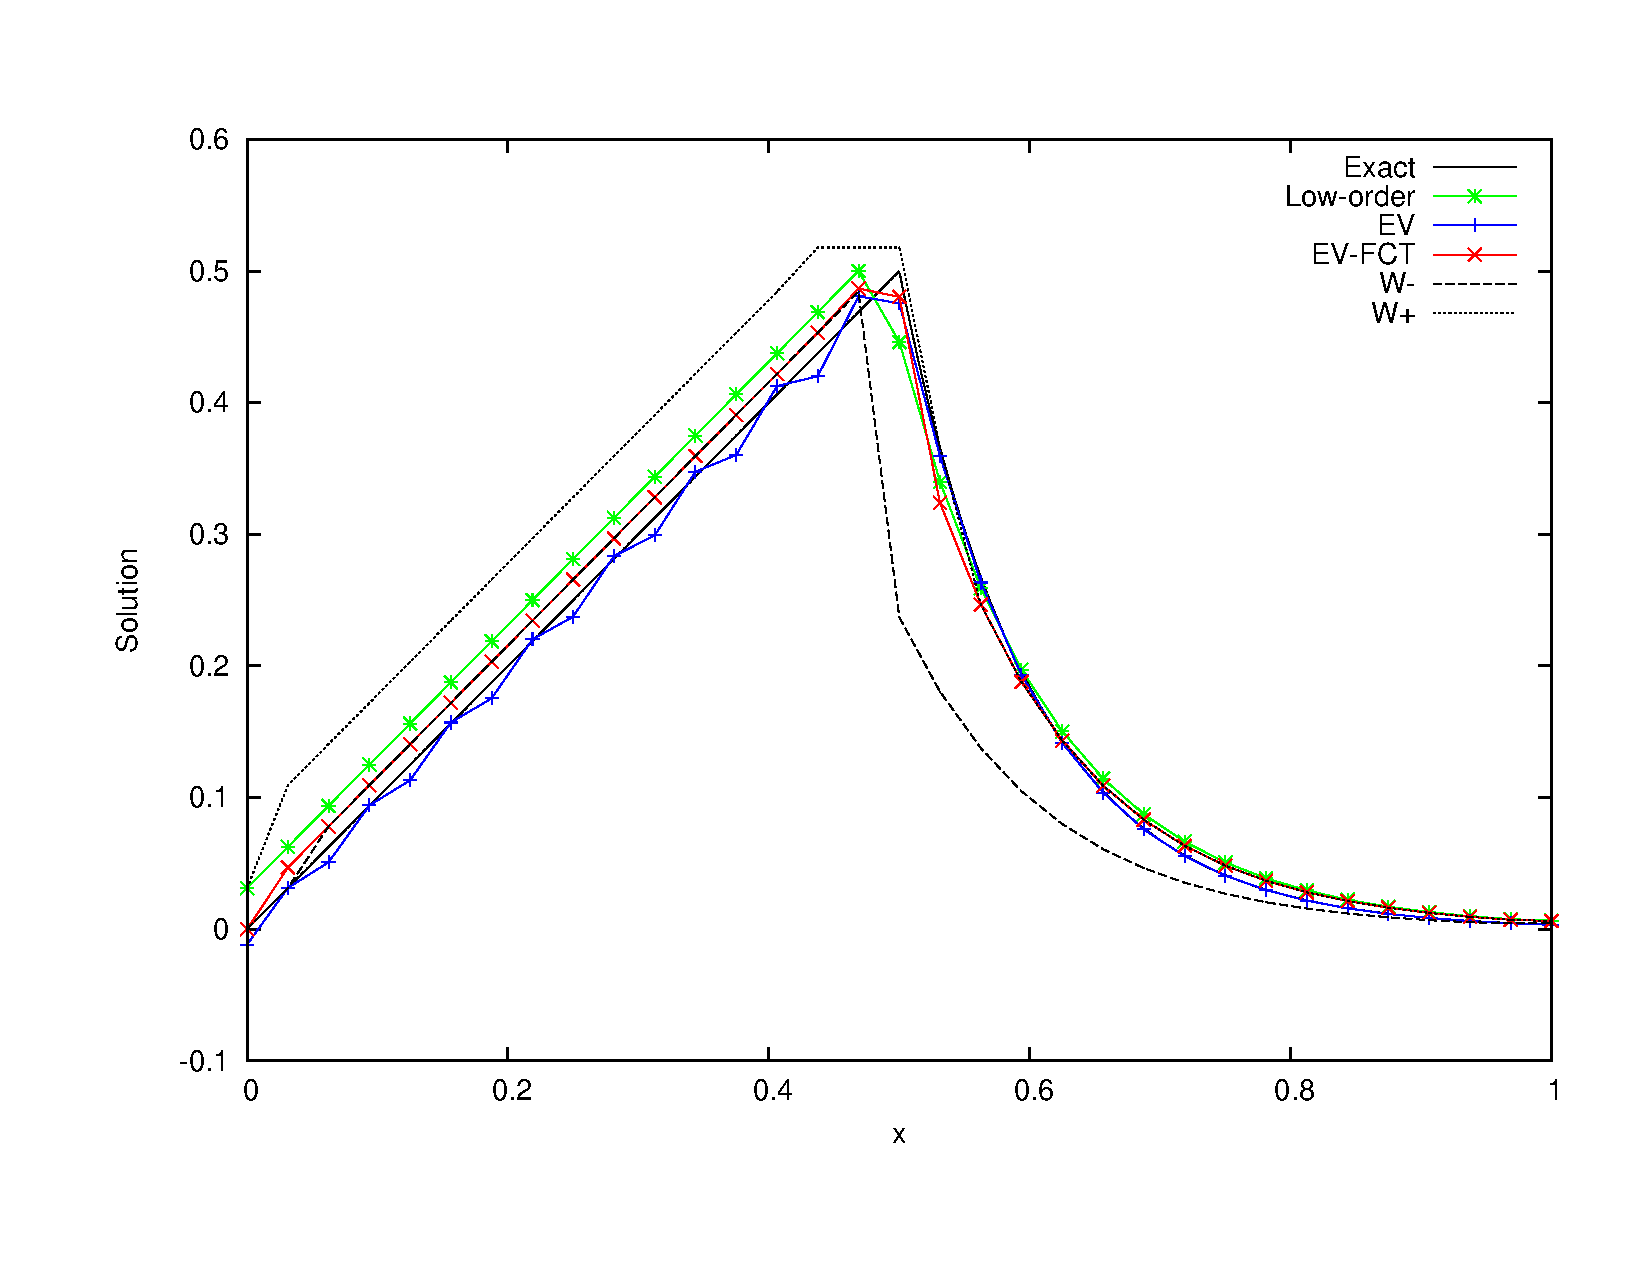
\includegraphics[width=\textwidth]
     {\contentdir/results/transport/source_void_to_absorber/images/weak.pdf}
   \caption{Steady-State Solutions for the Source-Void-to-Absorber Problem
     with Weakly Imposed Dirichlet Boundary Conditions}
   \label{fig:source_void_to_absorber_weak}
\end{figure}
%-------------------------------------------------------------------------------
%-------------------------------------------------------------------------------
\begin{figure}[ht]
   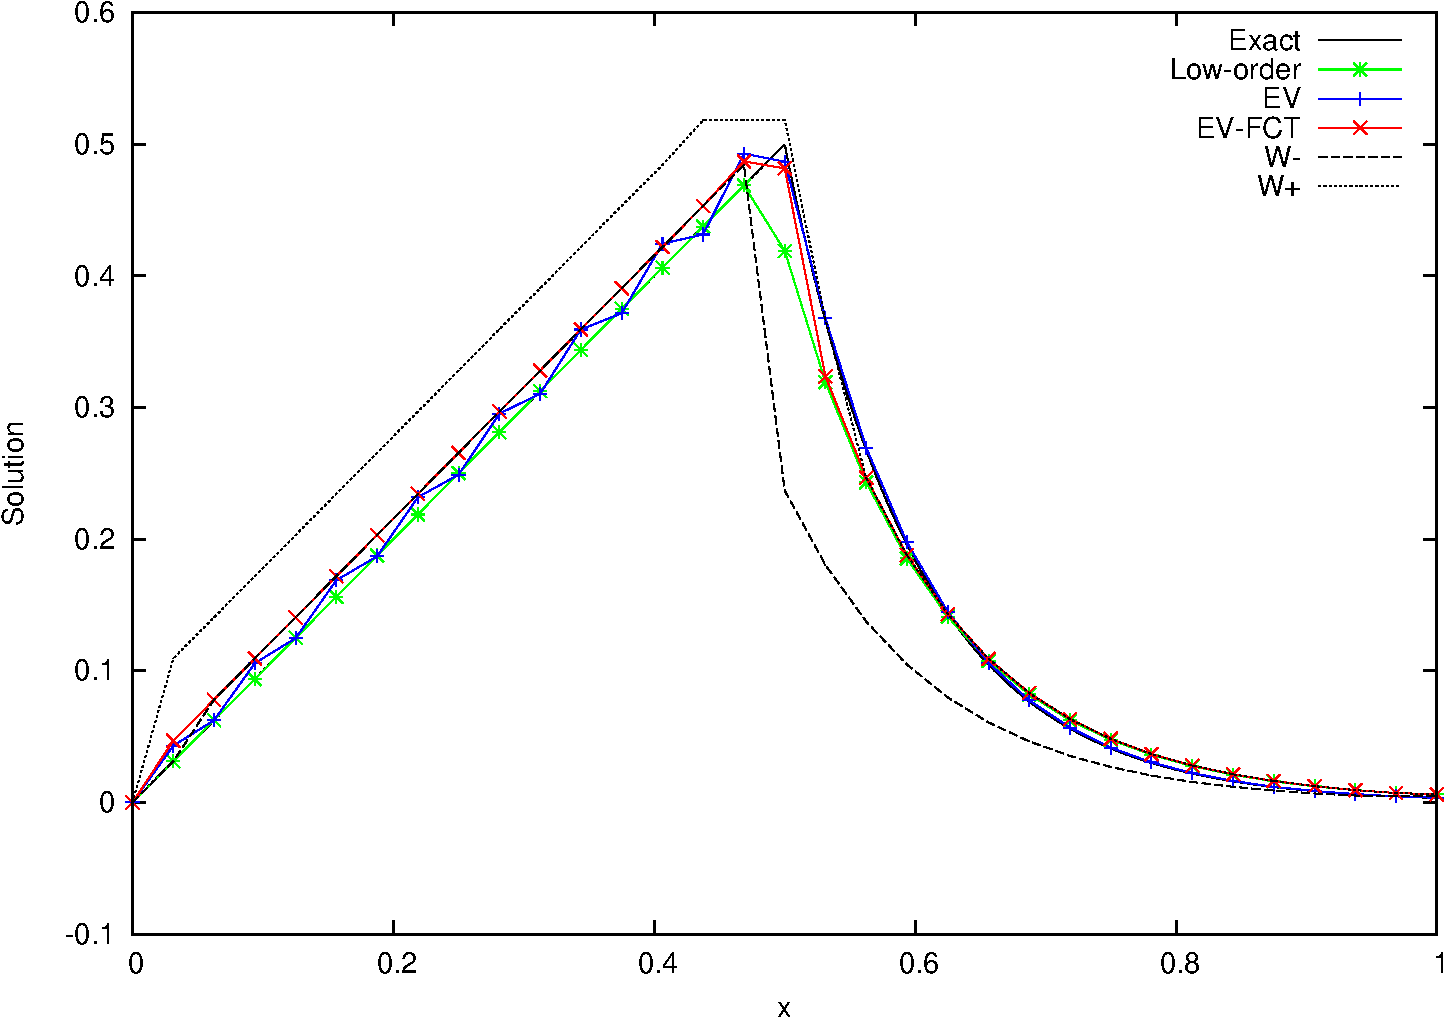
\includegraphics[width=\textwidth]
     {\contentdir/results/transport/source_void_to_absorber/images/weak_with_penalty.pdf}
   \caption{Steady-State Solutions for the Source-Void-to-Absorber Problem
     with Weakly Imposed Dirichlet Boundary Conditions and Boundary Penalty}
   \label{fig:source_void_to_absorber_penalty}
\end{figure}
%-------------------------------------------------------------------------------

Table \ref{tab:source_void_to_absorber_be_iterations_cells} shows the
results of a study of the number of EV and FCT iterations for
BE time discretization, required in
a transient with a constant CFL of 1 and varying mesh sizes. The
results in the table show a decrease in the number of EV iterations
per time step, and a relatively constant number of FCT iterations per
time step.

%-------------------------------------------------------------------------------
\begin{center}
\begin{table}[ht]
\caption{Nonlinear Iterations vs. Number of Cells for the
  Source-Void-to-Absorber Test Problem Using Implicit Euler Time Discretization
  with CFL = 1}
\label{tab:source_void_to_absorber_be_iterations_cells}
\begin{tabular}{c c c c c}\toprule
$N_{cell}$ & \multicolumn{2}{c}{\emph{EV}} & \multicolumn{2}{c}{\emph{FCT}}\\
           & \emph{Total} & \emph{Avg.}    &  \emph{Total} & \emph{Avg.}\\\midrule
  8 &  661 & 24.48 &   244 &  9.04\\
 16 &  807 & 19.21 &   655 & 15.60\\
 32 &  844 & 11.25 &  1194 & 15.92\\
 64 & 1204 &  8.72 &  2024 & 14.67\\
128 & 1752 &  6.59 &  3675 & 13.82\\
256 & 2713 &  5.20 &  6673 & 12.78\\
512 & 4284 &  4.14 & 12098 & 11.69\\
\bottomrule\end{tabular}
\end{table}
\end{center}
%-------------------------------------------------------------------------------

Table \ref{tab:source_void_to_absorber_be_iterations_cfl} shows
the results of a study of nonlinear iterations vs. CFL number for
implicit Euler time discretization and 128 cells. The general
trend shows that entropy viscosity iterations per time step gradually increase
with increasing CFL, while FCT iterations per time step increases
much more quickly. Even more problematic is that the EV-FCT solution
error jumps very quickly from CFLs $\nu=5$ to $\nu=10$.

%-------------------------------------------------------------------------------
\begin{table}[htb]
\caption{Nonlinear Iterations vs. CFL Number for the
 Source-Void-to-Absorber Test Problem Using Implicit Euler Time Discretization
 with 128 Cells}
\label{tab:source_void_to_absorber_be_iterations_cfl}
\centering
\begin{tabular}{c c c c c c c }\toprule
 & & \multicolumn{2}{c}{\emph{EV}}
  & \multicolumn{2}{c}{\emph{FCT}} &\\
\emph{CFL} & $N_{step}$ & \emph{Total} & \emph{Avg.}
  & \emph{Total} & \emph{Avg.} & $L^2$ \emph{err.}\\\midrule
0.1 & 2661 & 15006 &  5.64 & 14036 &   5.27 & $3.013\times10^{-3}$\\
0.5 &  533 &  3445 &  6.46 &  5000 &   9.38 & $3.033\times10^{-3}$\\
1.0 &  266 &  1752 &  6.59 &  3675 &  13.82 & $3.023\times10^{-3}$\\
5.0 &   54 &   471 &  8.72 & 12208 & 226.07 & $2.979\times10^{-3}$\\
10.0 &  27 &   232 &  8.59 &  6126 & 226.89 & $3.325\times10^{-3}$\\
20.0 &  14 &   133 &  9.50 &  3713 & 265.21 & $3.727\times10^{-3}$\\
50.0 &   6 &    62 & 10.33 &  2077 & 346.17 & $7.191\times10^{-3}$\\
\bottomrule\end{tabular}
\end{table}
%-------------------------------------------------------------------------------

\clearpage

In this section, results are presented for the
source-void-to-absorber test problem. This is a 1-D test problem
with zero incoming flux incident on the left boundary,
a constant source in a void in the left half of the
domain, and an absorber with no source in the right half of the
domain. The test problem description is given by Table
\ref{tab:source_void_to_absorber}.

%-------------------------------------------------------------------------------
\begin{table}[htb]\caption{Source-Void-to-Absorber Test Problem Summary}
\label{tab:source_void_to_absorber}
\centering
\begin{tabular}{l l}\toprule
\emph{Parameter} & \emph{Value}\\\midrule
Domain & $\domain = (0,1)$\\
Initial Conditions & $u_0(x)=0$\\
Boundary Conditions & $u(0,t)=0 \eqc \quad t>0$\\
Direction & $\di = \mathbf{e}_x$\\
Cross Section & $\sigma(x)=\left\{\begin{array}{c l}
   0,  & x < \frac{1}{2}\\
   10, & \mbox{otherwise}\end{array}\right.$\\
Source & $q(\x,t)=\left\{\begin{array}{c l}
   1,  & x < \frac{1}{2}\\
   0,  & \mbox{otherwise}\end{array}\right.$\\
Speed & $\speed=1$\\
Exact Solution & $u(x,t)=\left\{\begin{array}{l l}
   \scalarsolution_{\text{ss}}(x), & x-t<0\\
   0, & \mbox{otherwise}
   \end{array}\right.$ \\
   & $\scalarsolution_{\text{ss}}(x) =
       \left\{\begin{array}{l l}
          e^{-10(x-\frac{1}{2})}, & x\ge\frac{1}{2}\\
          1,                      & \mbox{otherwise}
       \end{array}\right.$\\
\bottomrule\end{tabular}
\end{table}
%-------------------------------------------------------------------------------

Figure \ref{fig:source_void_to_absorber}
shows the results for this problem using SSPRK time discretization,
a CFL of 0.5, and 32 cells.
Entropy residual and jump coefficients $\entropyresidualcoef$ and
$\entropyjumpcoef$ are both 1.
Table \ref{tab:source_void_to_absorber_run_parameters} summarizes the
run parameters to generate the results in this section.
Figure \ref{fig:source_void_to_absorber_fine} shows results
for a finer mesh (256 cells) that illustrates the shortcomings of Galerkin-FCT
vs. EV-FCT: Galerkin-FCT does not necessarily converge to the
entropy solution.

%-------------------------------------------------------------------------------
\begin{table}[ht]\caption{Source-Void-to-Absorber Test Problem Run Parameters}
\label{tab:source_void_to_absorber_run_parameters}
\centering
\begin{tabular}{l l}\toprule
\emph{Parameter} & \emph{Value}\\\midrule
Number of Cells & $N_{cell} = 32, 256$\\
End Time & $t = 1$\\
CFL Number & $\nu = 0.5$\\\midrule
Entropy Function & $\entropy(u) = \frac{1}{2}u^2$\\
Entropy Residual Coefficient & $\entropyresidualcoef = 1$\\
Entropy Jump Coefficient & $\entropyjumpcoef = 1$\\
\bottomrule\end{tabular}
\end{table}
%-------------------------------------------------------------------------------
\begin{figure}[ht]
   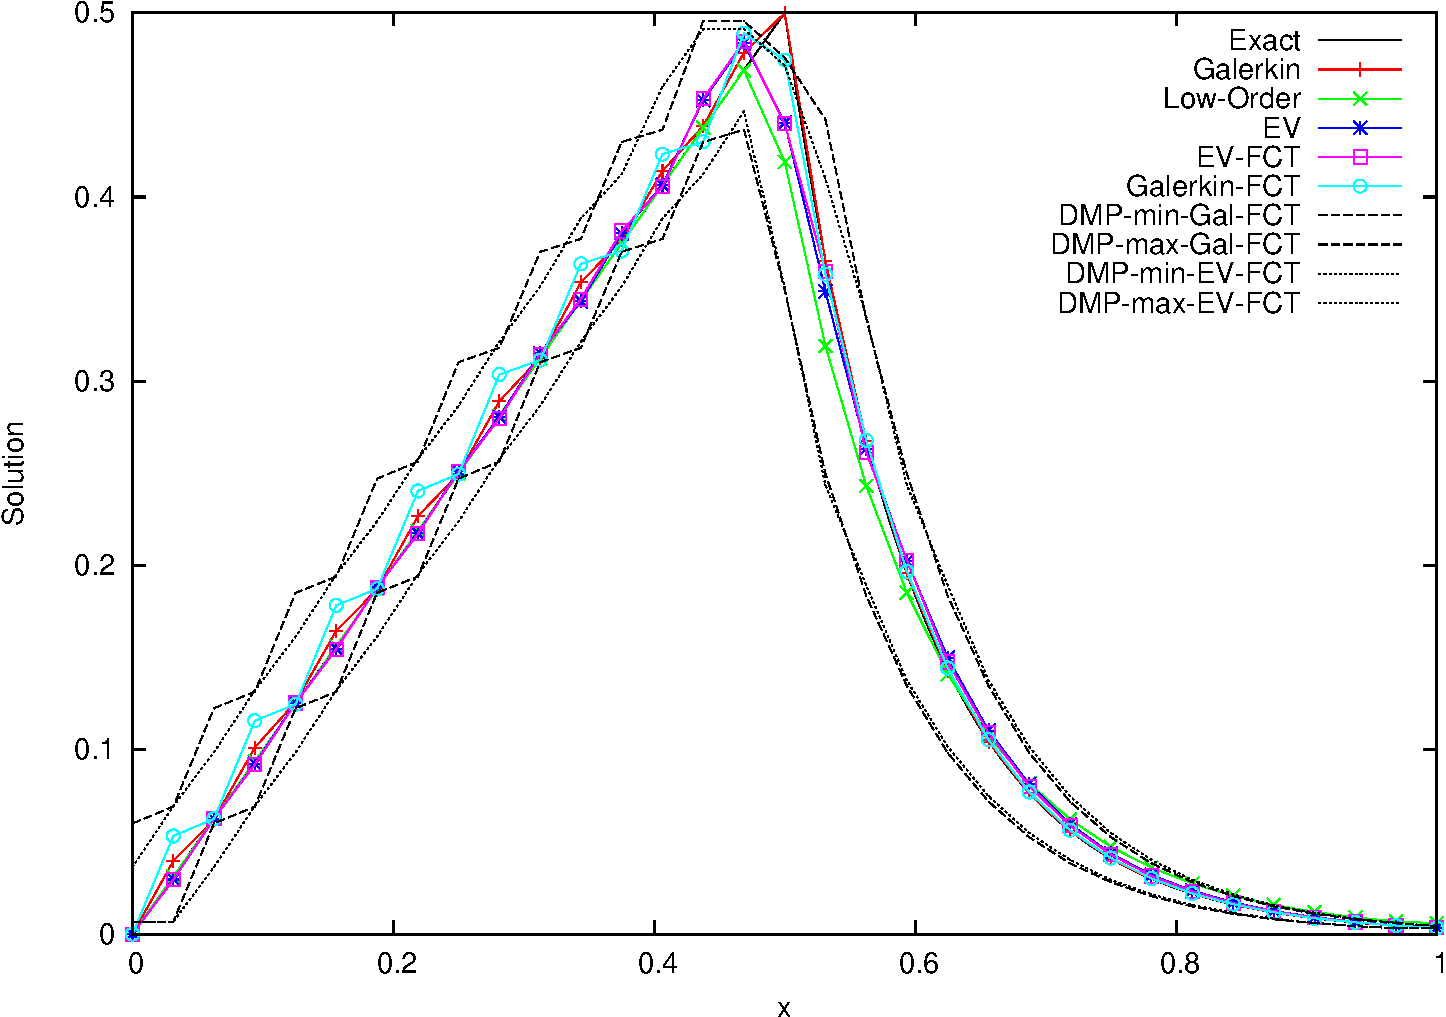
\includegraphics[width=\textwidth]
     {\contentdir/results/transport/source_void_to_absorber/coarse.pdf}
   \caption{Comparison of Solutions for the Source-Void-to-Absorber Problem
     Using SSPRK33 with 32 Cells}
   \label{fig:source_void_to_absorber}
\end{figure}
%-------------------------------------------------------------------------------
\begin{figure}[ht]
   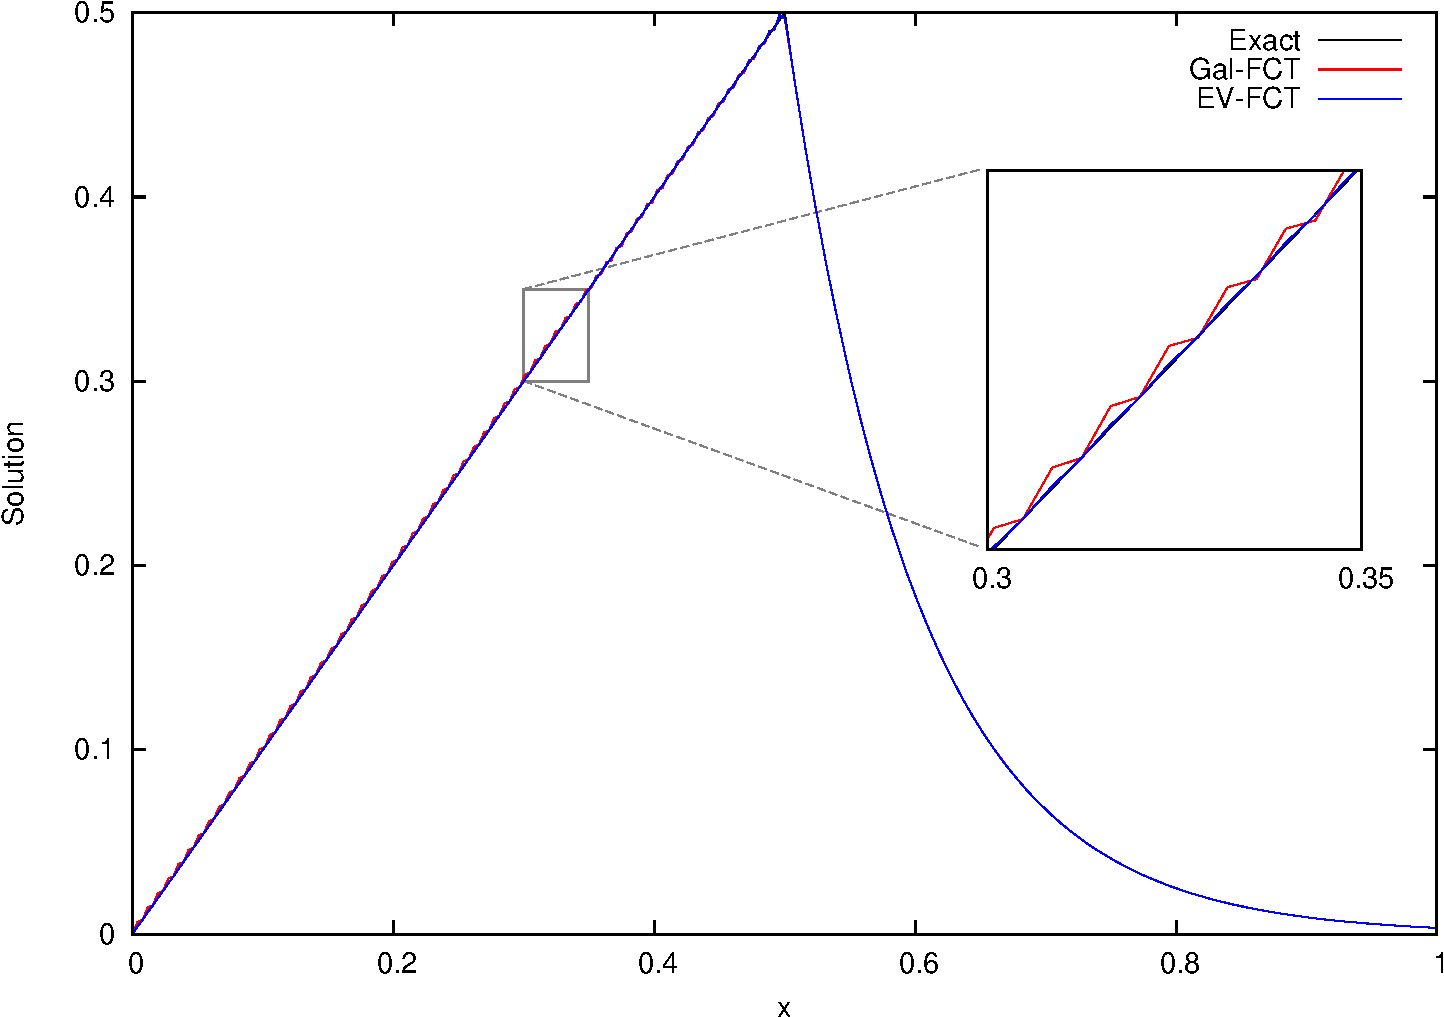
\includegraphics[width=\textwidth]
     {\contentdir/results/transport/source_void_to_absorber/fine.pdf}
   \caption{Comparison of Solutions for the Source-Void-to-Absorber Problem
     Using SSPRK33 with 256 Cells}
   \label{fig:source_void_to_absorber_fine}
\end{figure}
%-------------------------------------------------------------------------------

The steady-state results for this test problem revealed some significant
FCT issues regarding the antidiffusion from Dirichlet nodes.
When Dirichlet boundary conditions are strongly imposed, solution
bounds do not apply, and it becomes unclear how to limit antidiffusion
fluxes from these nodes. Consider symmetric limiters, i.e., those such that
$L\ij=L\ji$, such as Zalesak's limiter, for which
\begin{equation}
  L\ij = \left\{\begin{array}{c c}
    \min(L_i^+,L_j^-) & P\ij > 0\\
    \min(L_i^-,L_j^+) & P\ij < 0\\
  \end{array}\right. \eqp
\end{equation}
Suppose $i$ corresponds to a degree of freedom for which Dirichlet
boundary conditions are strongly imposed. The uncertainty
is the correct way to decide $L_i^+$ and $L_i^-$ since there
are no valid bounds from which to compute these values.
Figures \ref{fig:source_void_to_absorber_strong1} and 
\ref{fig:source_void_to_absorber_strong0} show the solutions obtained
using strongly imposed Dirichlet boundary conditions with these
values set to $L_i^+=L_i^-=1$ and $L_i^+=L_i^-=0$, respectively.
When $L_i^+=L_i^-=1$, the correction flux from the Dirichlet
DoF $i$, which is positive, has only the upper bound for $j$
to consider. The upper bound for $j$, which is inflated above the
analytical solution due to the source, does not restrict this
antidiffusion flux, and thus it is accepted fully to the unphysical
value. Due to the implicitness of the solution bounds, the lower solution
bound for $j$ is computed from this unphysical value and excludes the
possibility of antidiffusion back to the analytical solution. This
process continues with all of the other degrees of freedom.
When instead, $L_i^+=L_i^-=0$, the solution does not lie above
the analytical solution in the source region, but significant peak
clipping appears at the interface between the source and absorber
regions. It should be noted that there are combinations of limiting
coefficient values, each in the range $(0,1)$, that produce a more
accurate solution to this problem (without the peak clipping
and resulting inaccuracy in the absorber region); the problem is that Zalesak's
limiter (and in general, any practical limiter) is not optimal
in the sense that it maximizes the magnitude of antidiffusive flux.
One could in principle solve an optimization problem to select
limiting coefficients that maximize the antidiffusive flux, but this
is very expensive and thus not recommended for general use.

For weakly imposed Dirichlet boundary conditions, solution bounds
still apply, so limiting coefficients may be computed without special
consideration. However, one must now consider the possibility of
inaccurate boundary values.
Figures \ref{fig:source_void_to_absorber_weak} shows the steady-state 
solutions obtained using weakly imposed Dirichlet boundary conditions.
In this case, the antidiffusion flux from the boundary gets limited
(but not fully) due to the lower solution bound of the Dirichlet node.
Because some antidiffusion was accepted here, the peak reaches
a higher value than with the $L_i^+=L_i^-=0$ case.
Finally, Figure \ref{fig:source_void_to_absorber_penalty} shows
the steady-state solution obtained with weakly imposed Dirichlet
boundary conditions and a boundary penalty (see Section \ref{sec:transport_bc}).
The FCT solution looks very similar to the case without any penalty,
but the effect on the low-order and entropy viscosity solutions is
clear.

%-------------------------------------------------------------------------------
\begin{figure}[ht]
   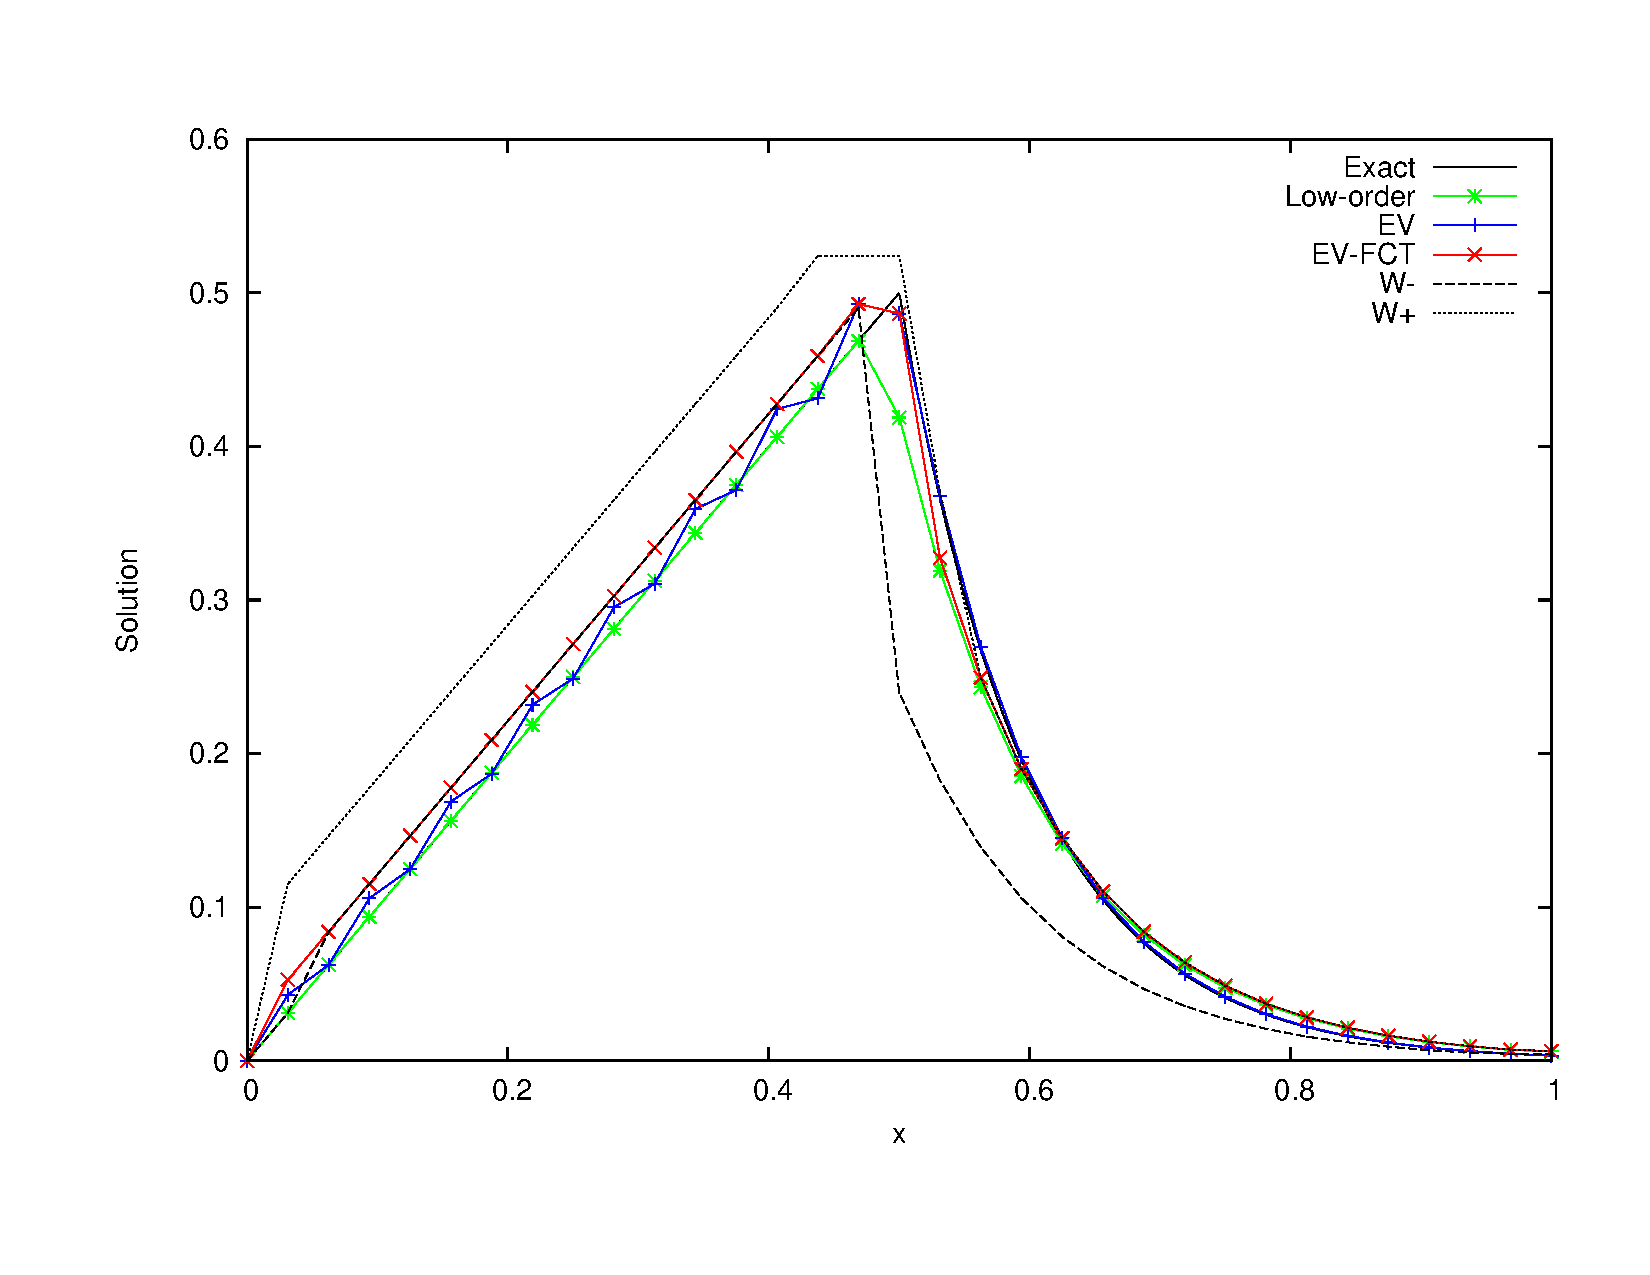
\includegraphics[width=\textwidth]
     {\contentdir/results/transport/source_void_to_absorber/images/strong1.pdf}
   \caption{Steady-State Solutions for the Source-Void-to-Absorber Problem
     with Strongly Imposed Dirichlet Boundary Conditions and $L^-=L^+=1$}
   \label{fig:source_void_to_absorber_strong1}
\end{figure}
%-------------------------------------------------------------------------------
%-------------------------------------------------------------------------------
\begin{figure}[ht]
   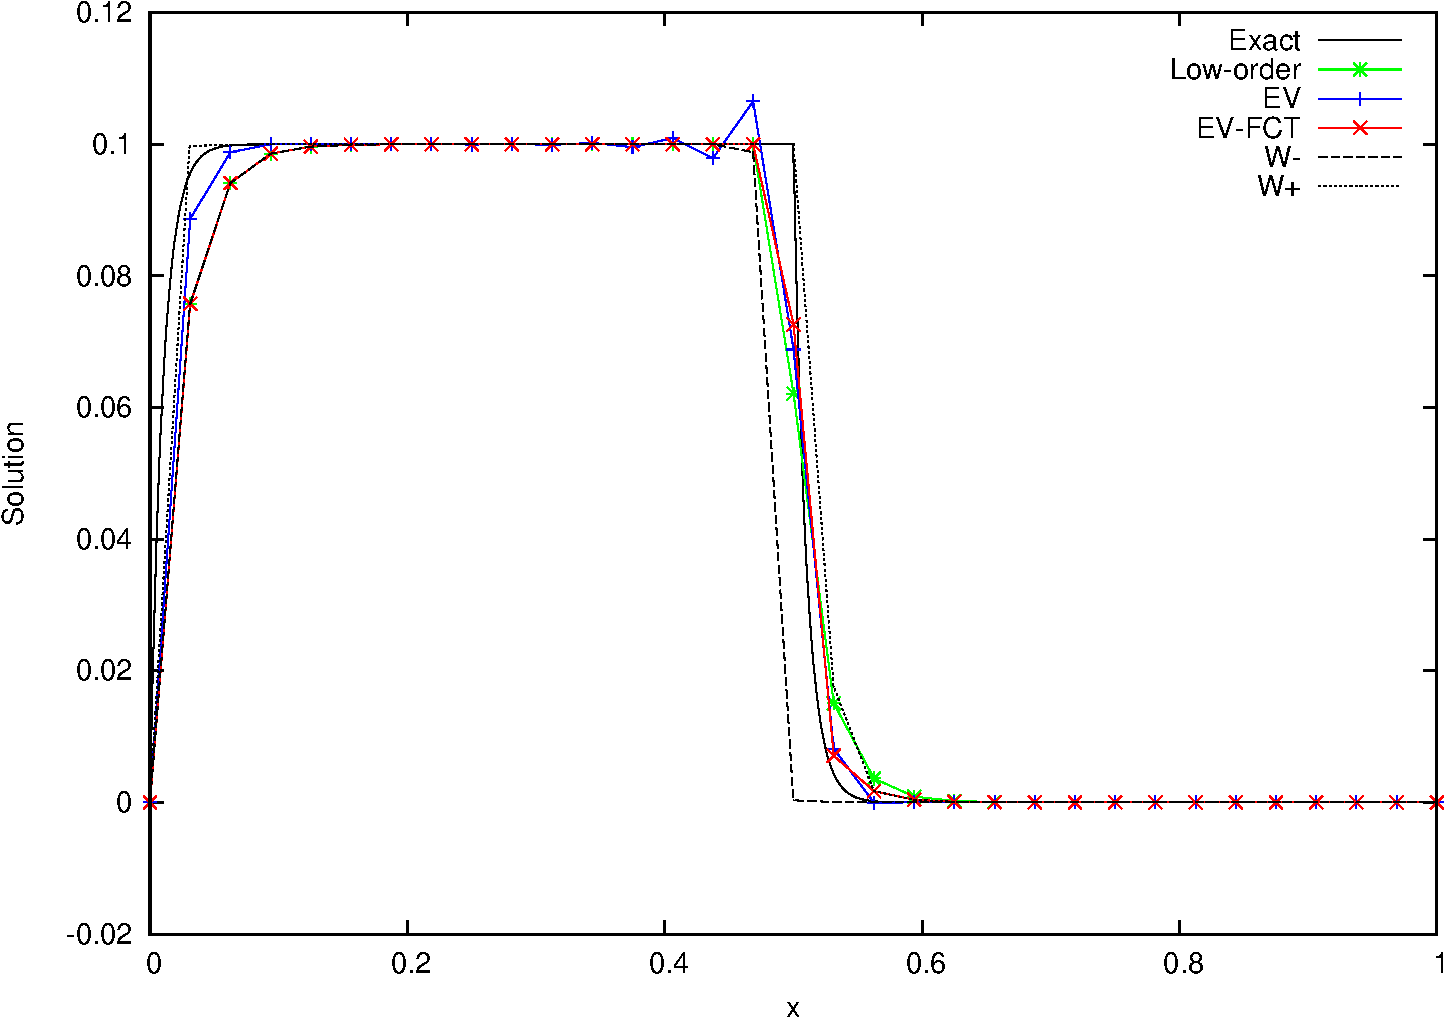
\includegraphics[width=\textwidth]
     {\contentdir/results/transport/source_void_to_absorber/images/strong0.pdf}
   \caption{Steady-State Solutions for the Source-Void-to-Absorber Problem
     with Strongly Imposed Dirichlet Boundary Conditions and $L^-=L^+=0$}
   \label{fig:source_void_to_absorber_strong0}
\end{figure}
%-------------------------------------------------------------------------------
%-------------------------------------------------------------------------------
\begin{figure}[ht]
   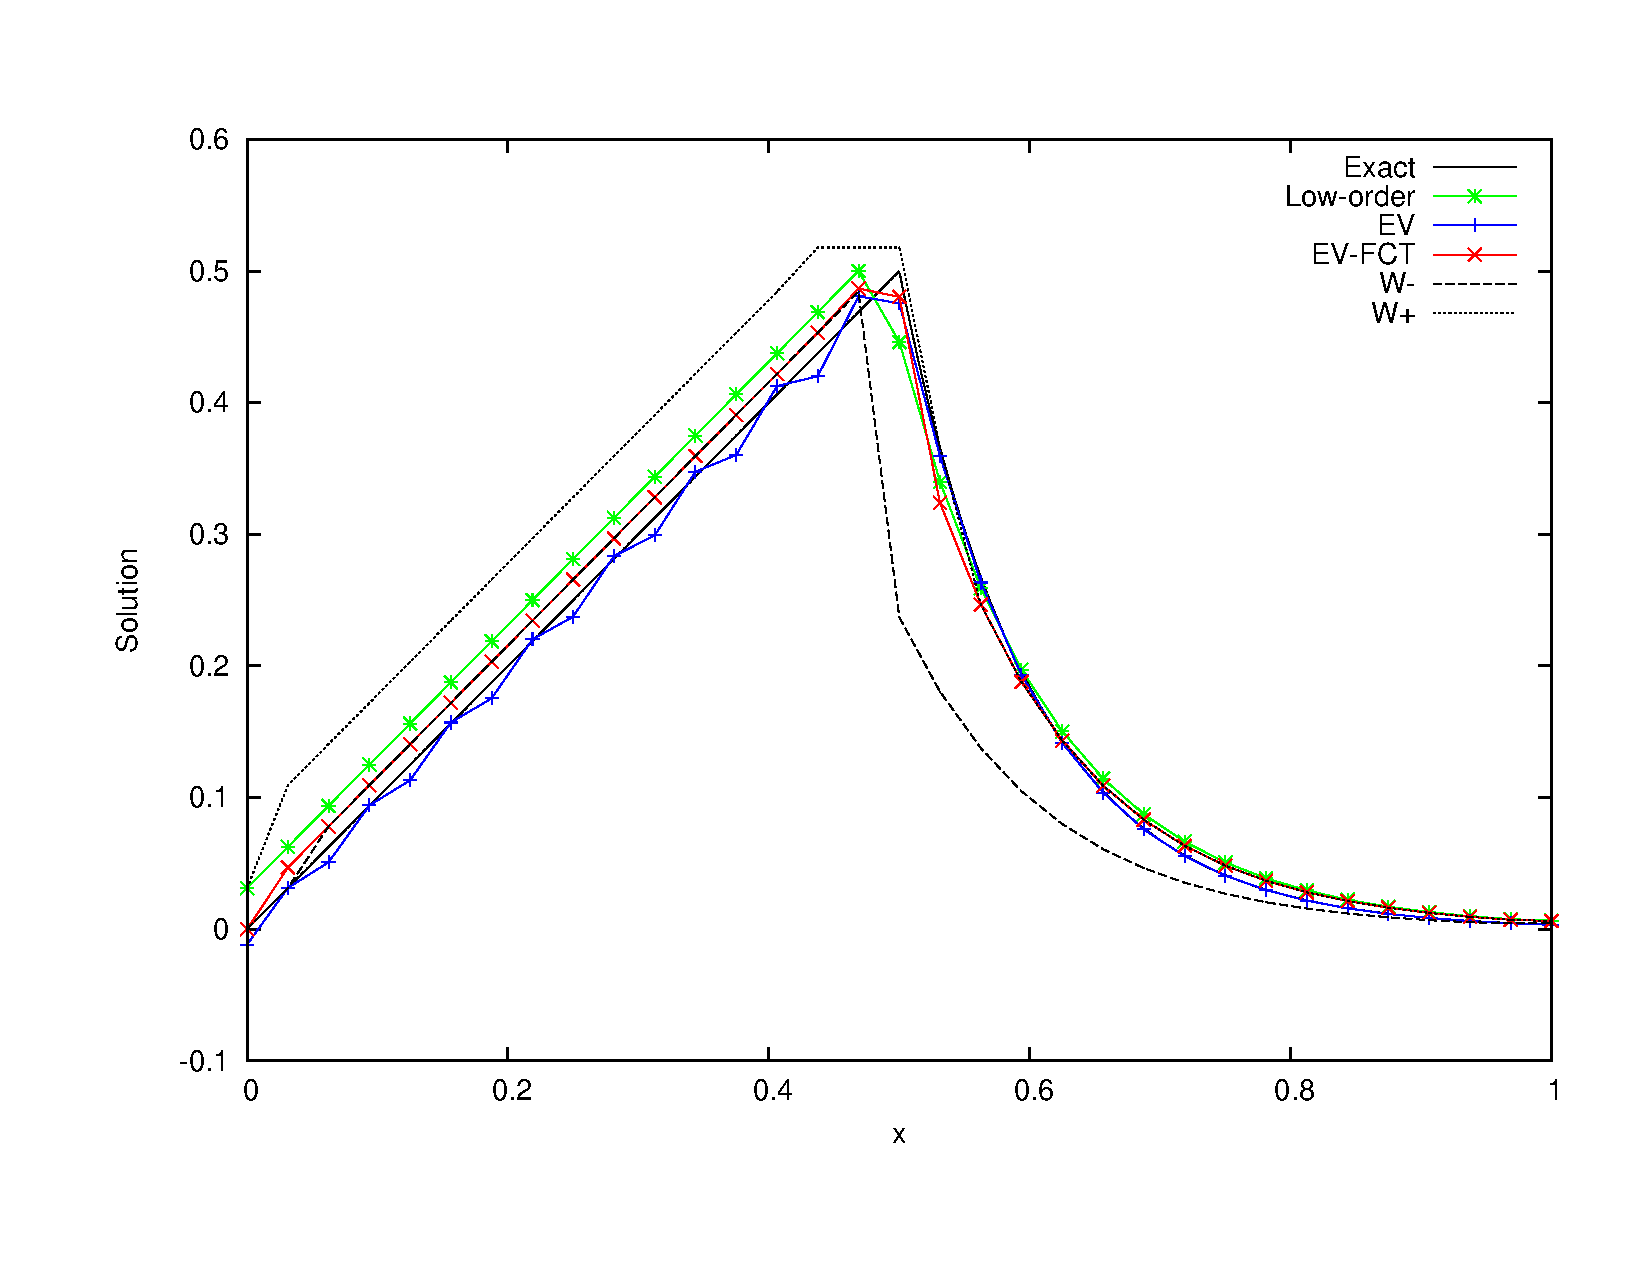
\includegraphics[width=\textwidth]
     {\contentdir/results/transport/source_void_to_absorber/images/weak.pdf}
   \caption{Steady-State Solutions for the Source-Void-to-Absorber Problem
     with Weakly Imposed Dirichlet Boundary Conditions}
   \label{fig:source_void_to_absorber_weak}
\end{figure}
%-------------------------------------------------------------------------------
%-------------------------------------------------------------------------------
\begin{figure}[ht]
   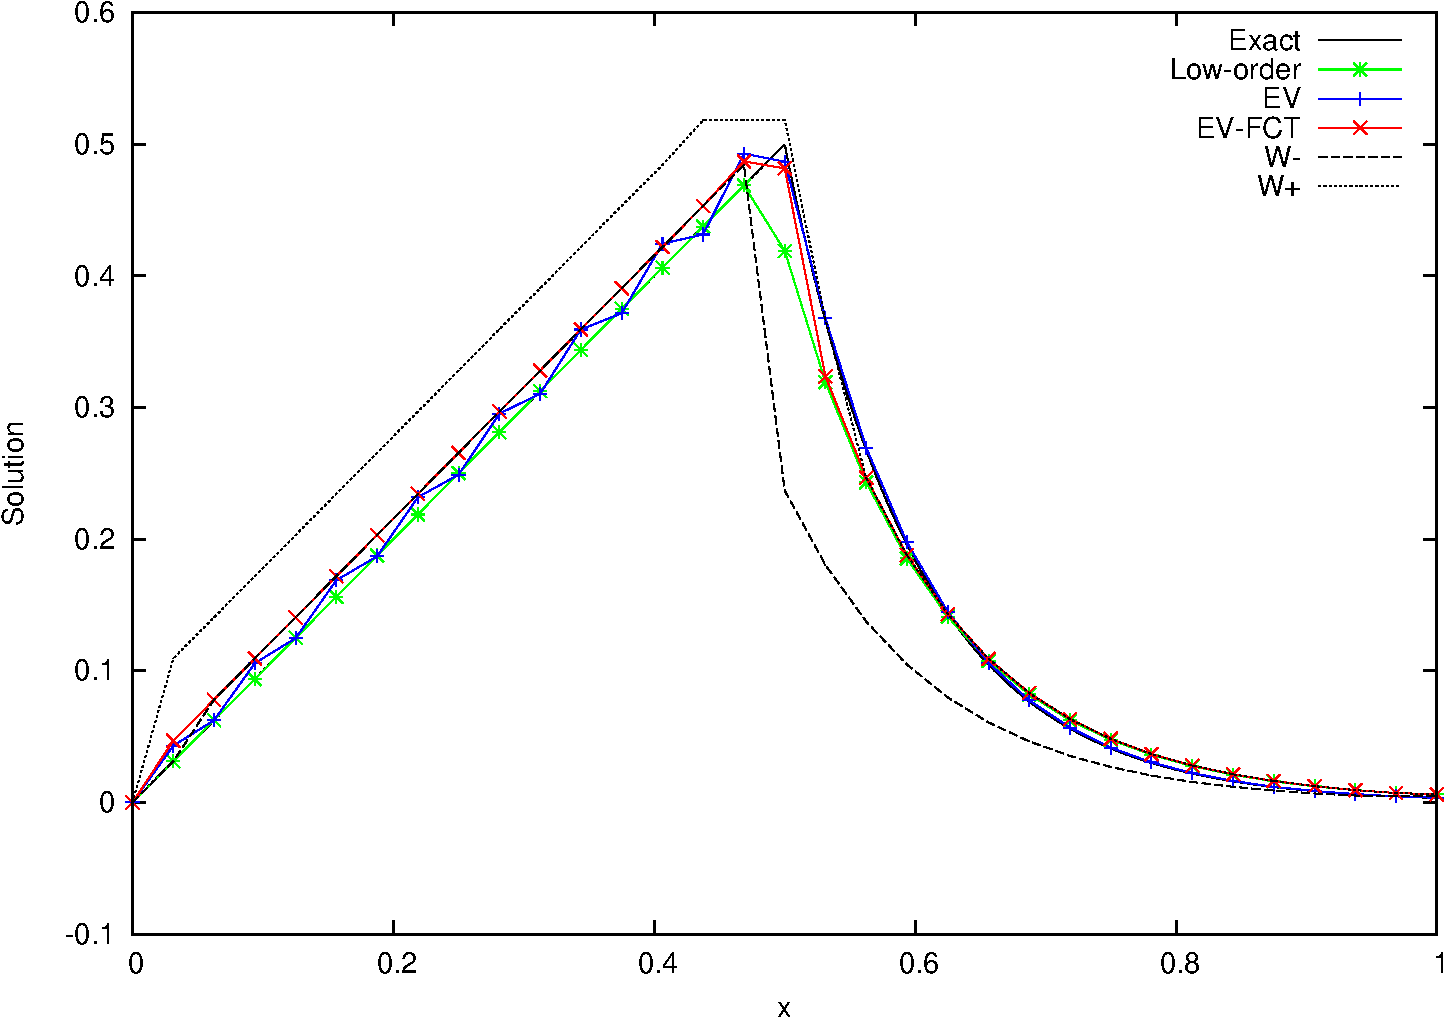
\includegraphics[width=\textwidth]
     {\contentdir/results/transport/source_void_to_absorber/images/weak_with_penalty.pdf}
   \caption{Steady-State Solutions for the Source-Void-to-Absorber Problem
     with Weakly Imposed Dirichlet Boundary Conditions and Boundary Penalty}
   \label{fig:source_void_to_absorber_penalty}
\end{figure}
%-------------------------------------------------------------------------------

Table \ref{tab:source_void_to_absorber_be_iterations_cells} shows the
results of a study of the number of EV and FCT iterations for
BE time discretization, required in
a transient with a constant CFL of 1 and varying mesh sizes. The
results in the table show a decrease in the number of EV iterations
per time step, and a relatively constant number of FCT iterations per
time step.

%-------------------------------------------------------------------------------
\begin{center}
\begin{table}[ht]
\caption{Nonlinear Iterations vs. Number of Cells for the
  Source-Void-to-Absorber Test Problem Using Implicit Euler Time Discretization
  with CFL = 1}
\label{tab:source_void_to_absorber_be_iterations_cells}
\begin{tabular}{c c c c c}\toprule
$N_{cell}$ & \multicolumn{2}{c}{\emph{EV}} & \multicolumn{2}{c}{\emph{FCT}}\\
           & \emph{Total} & \emph{Avg.}    &  \emph{Total} & \emph{Avg.}\\\midrule
  8 &  661 & 24.48 &   244 &  9.04\\
 16 &  807 & 19.21 &   655 & 15.60\\
 32 &  844 & 11.25 &  1194 & 15.92\\
 64 & 1204 &  8.72 &  2024 & 14.67\\
128 & 1752 &  6.59 &  3675 & 13.82\\
256 & 2713 &  5.20 &  6673 & 12.78\\
512 & 4284 &  4.14 & 12098 & 11.69\\
\bottomrule\end{tabular}
\end{table}
\end{center}
%-------------------------------------------------------------------------------

Table \ref{tab:source_void_to_absorber_be_iterations_cfl} shows
the results of a study of nonlinear iterations vs. CFL number for
implicit Euler time discretization and 128 cells. The general
trend shows that entropy viscosity iterations per time step gradually increase
with increasing CFL, while FCT iterations per time step increases
much more quickly. Even more problematic is that the EV-FCT solution
error jumps very quickly from CFLs $\nu=5$ to $\nu=10$.

%-------------------------------------------------------------------------------
\begin{table}[htb]
\caption{Nonlinear Iterations vs. CFL Number for the
 Source-Void-to-Absorber Test Problem Using Implicit Euler Time Discretization
 with 128 Cells}
\label{tab:source_void_to_absorber_be_iterations_cfl}
\centering
\begin{tabular}{c c c c c c c }\toprule
 & & \multicolumn{2}{c}{\emph{EV}}
  & \multicolumn{2}{c}{\emph{FCT}} &\\
\emph{CFL} & $N_{step}$ & \emph{Total} & \emph{Avg.}
  & \emph{Total} & \emph{Avg.} & $L^2$ \emph{err.}\\\midrule
0.1 & 2661 & 15006 &  5.64 & 14036 &   5.27 & $3.013\times10^{-3}$\\
0.5 &  533 &  3445 &  6.46 &  5000 &   9.38 & $3.033\times10^{-3}$\\
1.0 &  266 &  1752 &  6.59 &  3675 &  13.82 & $3.023\times10^{-3}$\\
5.0 &   54 &   471 &  8.72 & 12208 & 226.07 & $2.979\times10^{-3}$\\
10.0 &  27 &   232 &  8.59 &  6126 & 226.89 & $3.325\times10^{-3}$\\
20.0 &  14 &   133 &  9.50 &  3713 & 265.21 & $3.727\times10^{-3}$\\
50.0 &   6 &    62 & 10.33 &  2077 & 346.17 & $7.191\times10^{-3}$\\
\bottomrule\end{tabular}
\end{table}
%-------------------------------------------------------------------------------

\clearpage

\end{document}


\section{Conclusions\label{sec:conclusions}}
The FCT scheme described in this paper is second-order accurate in space,
converges to the entropy solution, and preserves non-negativity.
Spurious oscillations are mitigated but are not guaranteed to be
eliminated, as smaller magnitude oscillations may exist within the imposed
solution bounds.

% Local solution bounds imposed in the FCT algorithm were derived using the method
% of characteristics and integral transport equation.
% Two sets of solution
% bounds were considered, one considering only values along the upstream
% line segment traversed in a time step, and the other considering a spherical
% neighborhood that encompasses this line segment. The former set of solution
% bounds is much tighter, which has the advantage that there is a smaller range
% of limiting coefficient values that can be used, but has the disadvantage that
% there is less room for antidiffusion.

The traditional FCT phenomenon known as ``stair-stepping'',
``terracing'', or ``plateauing'' is still an open issue, particularly for
fully explicit temporal discretizations; however, these effects
have been shown to diminish or disappear when using SSPRK33 as opposed
to explicit Euler. In addition, these effects are less pronounced for EV-FCT
than in the classic FEM-FCT scheme, which uses the standard Galerkin method as
the high-order method in FCT.

The explicit temporal discretizations of the described FCT scheme yield a
relatively robust algorithm; however, implicit and steady-state discretizations
are much less robust, suffering from severe nonlinear convergence difficulties
in some problems. Implicit schemes become increasingly divergent as the CFL
number is increased. The main complication with implicit and steady-state
FCT schemes is that the imposed solution bounds are implicit with the solution,
and thus the imposed solution bounds change with each iteration of the
nonlinear solver.


\section*{References}
\bibliographystyle{elsarticle-num}
\bibliography{references}

\end{document}
